\documentclass[twoside=semi]{report}
\usepackage[
top    = 1cm,
bottom = 1cm,
footskip= 0cm, 
left   = 2cm,
right  = 2cm]{geometry}
\usepackage[czech, english]{babel}
\usepackage[T1]{fontenc}
\usepackage[utf8]{inputenc}

\usepackage[square, numbers]{natbib} % sazba pouzite literatury
\usepackage{indentfirst} % 1. odstavec jako v cestine, pro práci v aj možno zakomentovat
\usepackage{fancyhdr} % tisk hlaviček a patiček stránek
\usepackage{nomencl} % umožňuje snadno definovat zkratky a jejich seznam

% \usepackage{lmodern}
\usepackage{graphicx}
\usepackage{caption}
\usepackage{subcaption}
\usepackage{xspace}
\usepackage{enumerate}
\usepackage{enumitem}
\usepackage{bbding}
\usepackage[usenames,dvipsnames]{color} % barvy
\usepackage{url}
\usepackage{subscript}

\usepackage{tabularx}
\usepackage{pdflscape}
\usepackage{lipsum}
\usepackage{pdfpages}

\usepackage{courier}
\usepackage{float}
\usepackage{nonfloat}
\usepackage{wrapfig}

% utrzky kodu
\usepackage{listings,xcolor}
\usepackage{inconsolata}
\usepackage{algorithm}
\usepackage{algorithmicx} %slouží pro zápis algoritmů
\usepackage{algpseudocode} %slouží pro výpis pseudokódu
\usepackage{eqparbox}
\usepackage{dirtree}
\usepackage{array}
\usepackage{amsmath} % matematicke symboly
\usepackage{amsfonts}
\usepackage{amsxtra} % matematicka pismena
\usepackage{wasysym} % znak vyplnene sipky
\usepackage{setspace} % vyska radku
\usepackage{changepage} % zmena okraju stranky
% \usepackage{soul}
\usepackage{soulutf8}
\usepackage{datetime} % datum a cas
\usepackage{tabu} % vylepsene tabulky - ruzne siroke ohraniceni
\usepackage{pgfgantt}
\usepackage{textcomp}
\usepackage{pgfplots}
\usepackage{filecontents}
\usepackage{pgfplots}
\usepackage{tikz} % grafy
\usetikzlibrary{arrows,shapes,backgrounds,snakes,patterns,calc,trees,positioning,chains,shapes.geometric,decorations.pathreplacing,decorations.pathmorphing,matrix,shapes.symbols,pgfplots.groupplots}

% custom packages
\usepackage{spolecne/_lib/infodata} % info strings
\usepackage{spolecne/_lib/mathstyle}
\usepackage{spolecne/_lib/macros}
\usepackage{spolecne/_lib/colors} % barvy
\usepackage{spolecne/_lib/codestyle} % highlight zdrojovych kodu
\usepackage{spolecne/_lib/mathstyle} % matematicke pomocne fce

\usepackage{spolecne/_lib/qtree}

% code samples
\usepackage{listings}
\usepackage{courier}
%\lstset{basicstyle=\footnotesize\ttfamily,breaklines=true}
\lstset{
    basicstyle=\ttfamily\footnotesize,
    breaklines=true,
    frame=single, % adds a frame around the code
    xleftmargin=2cm,
    xrightmargin=2cm,
}

% exercises and solutions
\usepackage{mdframed}
\newmdenv[topline=false, bottomline=false, skipabove=\topsep, rightline=false,
  skipbelow=\topsep]{exercise}

% graphs
\usepackage{tikz}
\usetikzlibrary[topaths]

\title{Státnicové otázky oboru Softwarové Inženýrství}
\date{}
\author{https://github.com/pryx/oi-mszz}

\setlength{\parskip}{1em}

\begin{document}

\maketitle

%\include{PAL/PAL}
%\include{TAL/TAL}
%\include{KO/KO}
\chapter{Společná část}
%!TEX root=../oi-magistr-spolecne.tex
\section[PAL - Složitost, fronty, haldy]{Amortizovaná složitost. Prioritní fronty, haldy (binární, d-regulární, binomiální, Fibonacciho), operace nad nimi a jejich složitost.}

\paragraph{Amortizovaná složitost.} Amortizovaná časová složitost označuje časovou složitost algoritmu v sekvenci nejhorších možných vstupních dat. Na rozdíl od průměrné složitosti nevyužívá pravděpodobnosti a je proto zaručená \cite{algoritmy:amortizovanaslozitost}.

\textbf{Asymptotická} složitost je \textbf{deklarována na základě nejhorší} (nejlepší) možné \textbf{instance běhu} algoritmu, což \textbf{ale} není vždy vypovídající, protože \textbf{i nejhorší sekvence případů může mít výrazně lepší průběh}, než by asymptotická složitost napovídala. Tento zdánlivý paradox je zapříčiněn tím, že operace s vysokou složitostí změní datovou strukturu tak, že takto špatný případ nenastane po nějakou delší dobu - tím se složitá operace amortizuje.

Jako jednoduchý příklad můžeme uvést specifickou implementaci dynamického pole, která zdvojnásobuje velikost pole pokaždé, když dojde k jeho naplnění. V tomto případě je tedy nutná realokace, v nejhorším případě tato operace potřebuje čas až $O(n)$ - což je asymptotická složitost. Samotné vkládání prvků (bez nutnosti realokace) vyžaduje čas $O(1)$, pro $n$ prvků tedy také $O(n)$. Pro vložení $n$ prvků (včetně realokace) je tedy potřeba $O(n) + O(n) = O(n)$, amortizovaný čas na jedno vložení prvku je pak $O(n)/n = O(1)$ \cite{wiki:amortizovana}.

\paragraph{Definice.} Je dána datová struktura $D$, na které postupně provádíme posloupnost stejných operací. Začneme s $D_0 = D$. První operace zavolaná na $D_0$ upraví datovou strukturu na $D_1$. Druhá operace zavolaná na $D_1$ upraví datovou strukturu na $D_2$. A tak dále. Postupně zavoláme $i$-tou operaci na $D_{i-1}$ a ta upraví datovou strukturu na $D_i$. Některá operace může trvat krátce, jiná déle. Průměrný čas doby trvání operace nazveme amortizovanou časovou složitostí. Amortizovanou časovou složitost jedné operace spočítáme tak, že spočteme celkovou časovou složitost posloupnosti operací v nejhorším případě a vydělíme ji počtem operací.

K čemu je amortizovaná časová složitost? Pomůže nám lépe odhadnout časovou složitost některých algoritmů v nejhorším případě \cite{algoritmyeu:amortizovana}.

\begin{itemize}[itemsep=0pt, topsep=0pt]
    \item Účetní metoda
    \item Metoda potenciálu
\end{itemize}

\noindent Interaktivní struktury: \url{https://www.cs.usfca.edu/~galles/visualization/Algorithms.html}

\subsection{Prioritní fronta \textit{(Priority Queue)}}
Prioritní fronta je \textit{abstraktní datový typ}, podobný klasické frontě či zásobníku s tím rozdílem, že každý element má svou \uv{prioritu}. V prioritní frontě je element s vyšší prioritou vybrán dříve než element s nižší prioritou. Pokud dva elementy mají stejnou prioritu, vyberou se v pořadí v jakém byly vloženy.

\paragraph{Operace.} Prioritní fronta musí implementovat alespoň následující operace:

\begin{itemize}[itemsep=0pt, topsep=2pt]
    \item[-] \texttt{void push(Element e)} - vloží element do prioritní fronty
    \item[-] \texttt{Element pull()} - vybere z fronty element s nejvyšší prioritou
\end{itemize}

\subsection{Haldy}
Halda (minimální) obecně je datová struktura (obvykle stromová) splňující \textbf{vlastnost haldy}:

\begin{center}
    \textit{Pokud B je potomek A, pak B $\geq$ A}
\end{center}

\subsubsection*{Binární halda (Binary heap)}
(Minimální) binární halda je binární strom s dvěma dalšími omezeními:

\begin{enumerate}[itemsep=0pt, topsep=2pt]
    \item Je to kompletní binární strom krom posledního patra (nemusí být úplné). Elementy posledního patra se plní zleva doprava.
    \item Každý element je menší nebo roven vůči jeho potomkům (vlastnost haldy).
\end{enumerate}

\noindent Je to jedna z možných implementací prioritní fronty. Reprezentovat ji můžeme pomocí pole (obr. \ref{fig:heap_array_representation}), kde prvek na indexu (číslováno od 1) $i$ má potomky na indexech $2i$ a $2i + 1$ a rodiče na indexu $i/2$.

\begin{figure}[htbp]
    \begin{center}
        \vspace{-20px}
        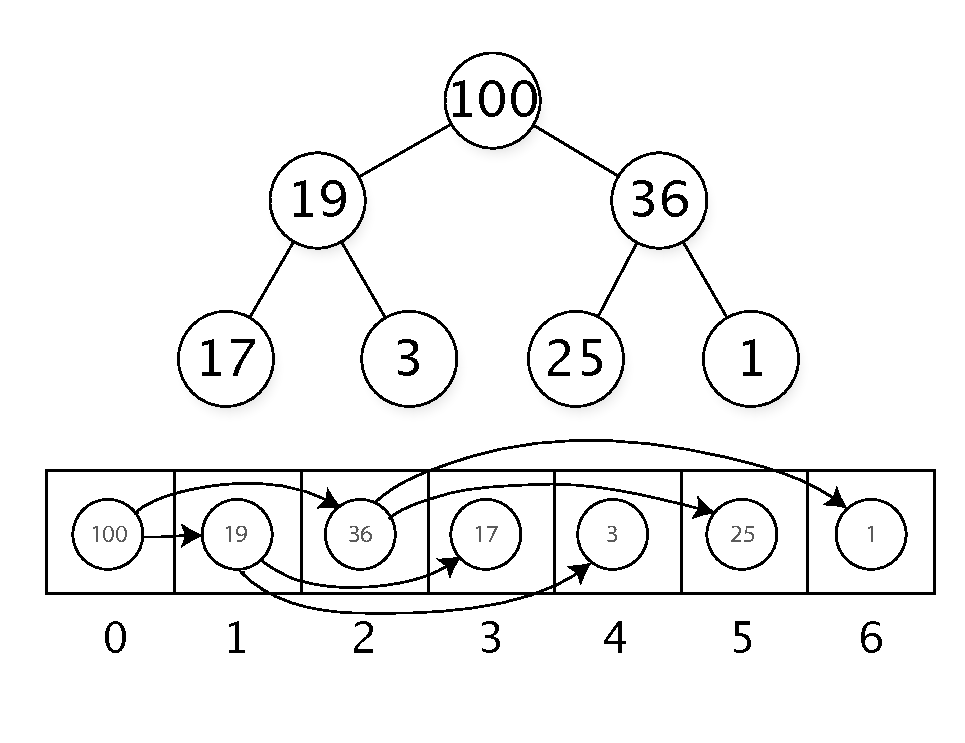
\includegraphics[width=100mm]{spolecne/01/images/Max-Heap}
        \vspace{-20px}
        \caption{Reprezentace (maximální) binární haldy v poli}
        \label{fig:heap_array_representation}
        \vspace{-20px}
    \end{center}
\end{figure}

\paragraph{Operace.} Operace binární haldy a jejich složitosti:

\begin{itemize}[itemsep=0pt, topsep=2pt]
    \item \texttt{accessMin()} - vrátí hodnotu kořene stromu (typicky první prvek pole)
    \item \texttt{deleteMin(e)} - vrátí element \texttt{e}, který je kořenem stromu, na jeho místo vloží nejpravější prvek \texttt{y} ze spodního patra a poté, pokud je \texttt{y} větší než jeho nejmenší potomek, prohazuji \texttt{y} s jeho nejmenším potomkem do té doby, dokud je \texttt{y} větší než jeho nově vzniknuvší nejmenší potomek,  (tzv. \texttt{y} probublává stromem dolů).
    \item \texttt{insert(e)} - přidáme element \texttt{e} na konec haldy a dokud je předek větší než \texttt{e}, tak je prohazujeme (probublávání směrem nahoru).
    \item \texttt{delete(e)} - podobně jako \texttt{deleteMin()}, odeberu element \texttt{e} a nechám ho probublat
    \item \texttt{merge(h1, h2)} - sloučí 2 haldy, vytvoří nové pole, kam nakopíruje obsah obou hald a na toto nové pole zavolá proceduru \texttt{heapify()}. Ta jede od půlky pole směrem na začátek (navštíví všechny podhaldy) a každý vrchol podhaldy nechá probublat a správně zařadit.
    \item \texttt{decreaseKey(k, v)} - zmenšíme hodnotu elementu s klíčem \texttt{k} o \texttt{v} a necháme probublat stromem.
\end{itemize}

\begin{table}[ht]
    \centering
    \vspace{0px}
    \begin{tabu}{|[1pt]c|c|c|[1pt]}
        \tabucline[1pt]{-}
        operace & čas. složitost & poznámka \\\tabucline[1pt]{-}
        \texttt{accessMin()} & $\Theta (1)$ &  \textcolor{gray}{přístup k vrcholu haldy} \\\hline
        \texttt{deleteMin()} & $\Theta (\log(n))$ &  \textcolor{gray}{smazání vrcholu haldy} \\\hline
        \texttt{insert(e)} & $\Theta (\log(n))$ &  \textcolor{gray}{přidání prvku do haldy} \\\hline
        \texttt{delete(e)} & $\Theta (\log(n))$ &  \textcolor{gray}{smazání elementu haldy} \\\hline
        \texttt{merge(h1,h2)} & $\Theta (n_1 + n_2)$ &  \textcolor{gray}{sloučení 2 hald} \\\hline
        \texttt{decreaseKey(k,v)} & $\Theta (\log(n))$ &  \textcolor{gray}{snížení hodnoty klíče $k$ o $v$} \\\hline
    \end{tabu}
    \caption{Binární halda - Operace a jejich složitosti}
\label{table:bin_heap_complexity}
\end{table}

\subsubsection{D-regulární halda (D-ary heap)}
D-regulární halda je zobecnění binární haldy, kde počet potomků se rovná číslu $d$, namísto 2 jako je tomu v haldě binární. $d$ nám udává počet štěpení stromu haldy. Operace jsou identické jako v binární haldě. Časová složitost operací je téměř stejná, liší se jen v základu logaritmu (u binární haldy je základ 2, tady $d$). Pro efektivní implementaci je vhodné zvolit $d$ jako mocninu 2. V tomto případě lze totiž využít bitových posunů - změna indexu při průchodu polem. D-halda běží rychleji než binární pokud velikost haldy převyšuje velikost cache počítače \cite{pal:prednasky}.

\paragraph{Operace.} Operace d-regulární haldy a jejich složitosti:
\begin{table}[ht]
    \centering
    \vspace{0px}
    \begin{tabu}{|[1pt]c|c|c|[1pt]}
        \tabucline[1pt]{-}
        operace & čas. složitost & poznámka \\\tabucline[1pt]{-}
        \texttt{accessMin()} & $\Theta (1)$ &  \textcolor{gray}{přístup k vrcholu haldy} \\\hline
        \texttt{deleteMin()} & $\Theta (\log_d(n))$ &  \textcolor{gray}{smazání vrcholu haldy} \\\hline
        \texttt{insert(e)} & $\Theta (\log_d(n))$ &  \textcolor{gray}{přidání prvku do haldy} \\\hline
        \texttt{delete(e)} & $\Theta (\log_d(n))$ &  \textcolor{gray}{smazání elementu haldy} \\\hline
        \texttt{merge(h1,h2)} & $\Theta (n_1 + n_2)$ &  \textcolor{gray}{sloučení 2 hald} \\\hline
        \texttt{decreaseKey(k,v)} & $\Theta (\log_d(n))$ &  \textcolor{gray}{snížení hodnoty klíče $k$ o $v$} \\\hline
    \end{tabu}
    \caption{D-regulární halda - Operace a jejich složitosti}
\label{table:d_heap_complexity}
\end{table}

\subsubsection{Binomiální halda (Binomial heap)}
Binomiální halda je kolekce binomiálních stromů stupňů $i = 0 \hdots \lfloor \log(n) \rfloor$. Každý řád je zastoupen maximálně 1 stromem.

\paragraph{Binomiální strom} je definovám rekurzivně:

\begin{itemize}[itemsep=0pt, topsep=2pt]
    \item Binomiální strom řádu 0 obsahuje jediný prvek - kořen
    \item Binomiální strom řádu $k$ má kořenový element, jehož potomci jsou kořeny binomiálních stromů stupňů $k-1, k-2, \hdots, 2, 1, 0$ (v tomto pořadí)
\end{itemize}

\begin{wrapfigure}{r}{0.55\textwidth}
    \vspace{-20px}
    \begin{center}
        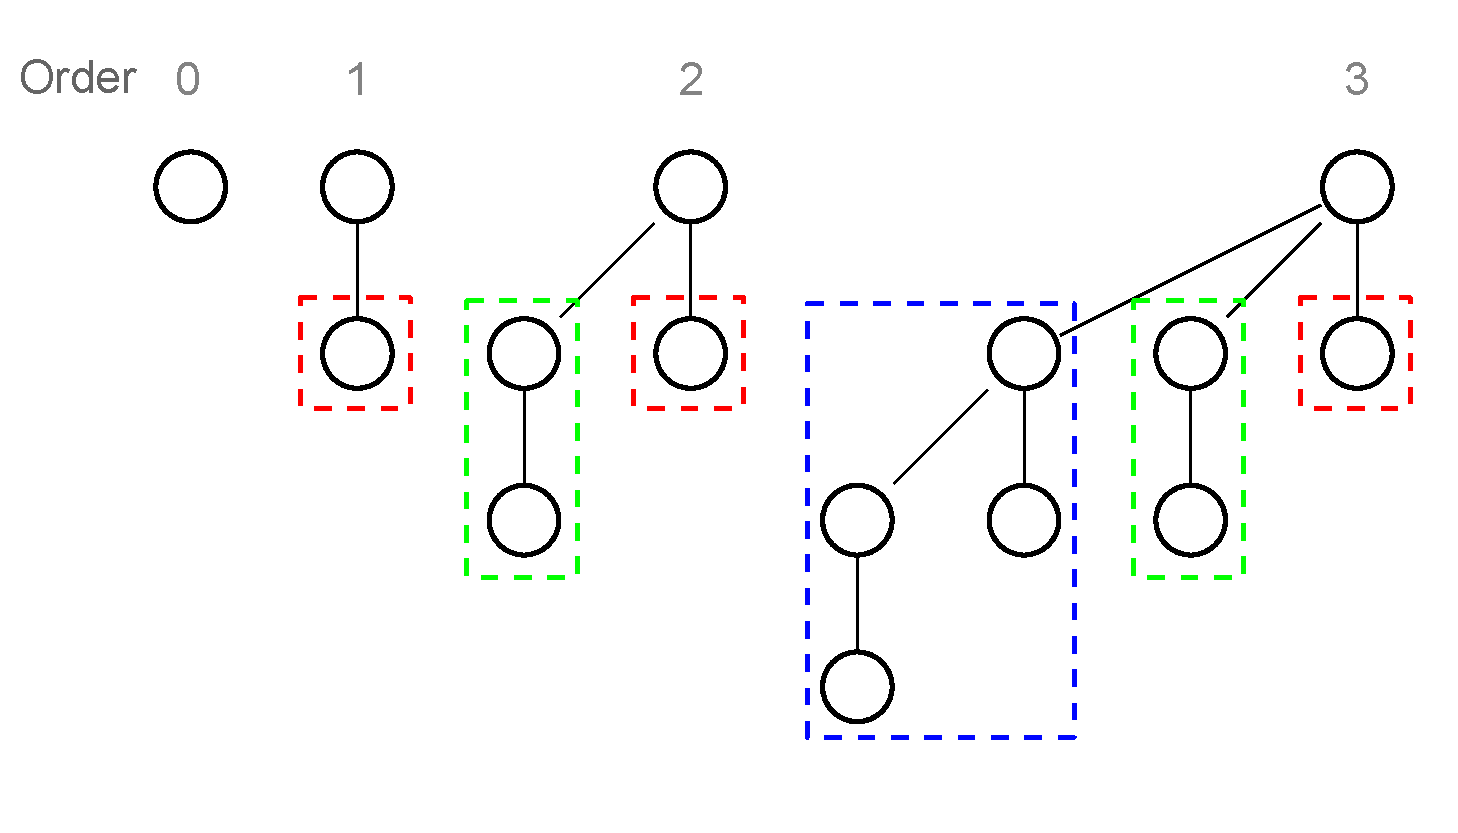
\includegraphics[width=65mm]{spolecne/01/images/Binomial_Trees}
    \end{center}
    \vspace{-30pt}
    \label{fig:binom_heap}
    \vspace{-60pt}
\end{wrapfigure}

\noindent Pro binomiální strom řádu $k$ platí:

\begin{itemize}[itemsep=0pt, topsep=2pt]
    \item splňuje vlastnost haldy
    \item hloubka stromu je $k$
    \item kořen má $k$ potomků
    \item obsahuje $2^k$ prvků
\end{itemize}

\paragraph{Operace.} Operace binomiální haldy a jejich složitosti:

\begin{itemize}[itemsep=0pt, topsep=2pt]
    \item \texttt{accessMin()} - vrátí kořen binomiálního stromu z MIN ukazatele.
    \item \texttt{deleteMin(e)} - vezmou se všechny podstromy, které vznikly odebráním kořene a ty se postupně mergují s ostatními stromy
    \item \texttt{insert(e)} - z vkládaného prvku se vytvoři nová binomiální halda (strom řádu 0) a ta se merguje s původní haldou
    \item \texttt{delete(e)} - sníží se hodnota pomocí \texttt{decreaseKey} na $-\infty$ a provede se \texttt{deleteMin()}
    \item \texttt{merge(h1, h2)} - Analogie mezi mergeováním dvou hald a binárním sčítáním. Naskládáme si stromy obou hald pod sebe (podle jejich stupňů). Pokud v jedné haldě je strom $i$-tého řádu a v druhé není, tak ho jen opíši. Pokud v obou haldách existují stromy stejného řadu, pak vzniká přenos do vyššího řádu. Kdykoliv vznikne přenos, mergujeme tyto dva stromy do sebe. Díky struktuře stromů, se provádí merge, porovnáním jejich kořenů, menší z kořenů se stane kořenem nově vzniklého stromu (řádu o 1 vyšší) a druhý strom se stane jeho potomkem.
    \item \texttt{decreaseKey(k, v)} - podobné jako u binární haldy
\end{itemize}

\begin{figure}[htbp]
    \begin{center}
        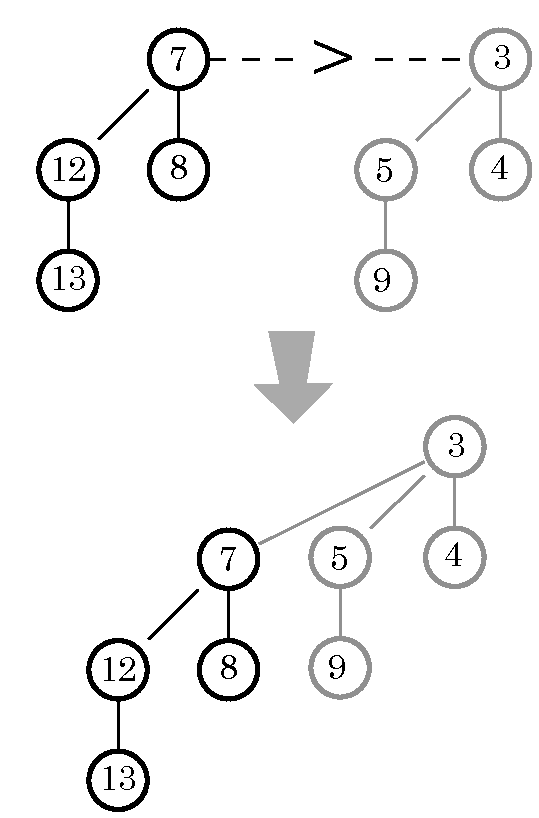
\includegraphics[width=45mm]{spolecne/01/images/Binomial_heap_merge1}
        \hspace{50px}
        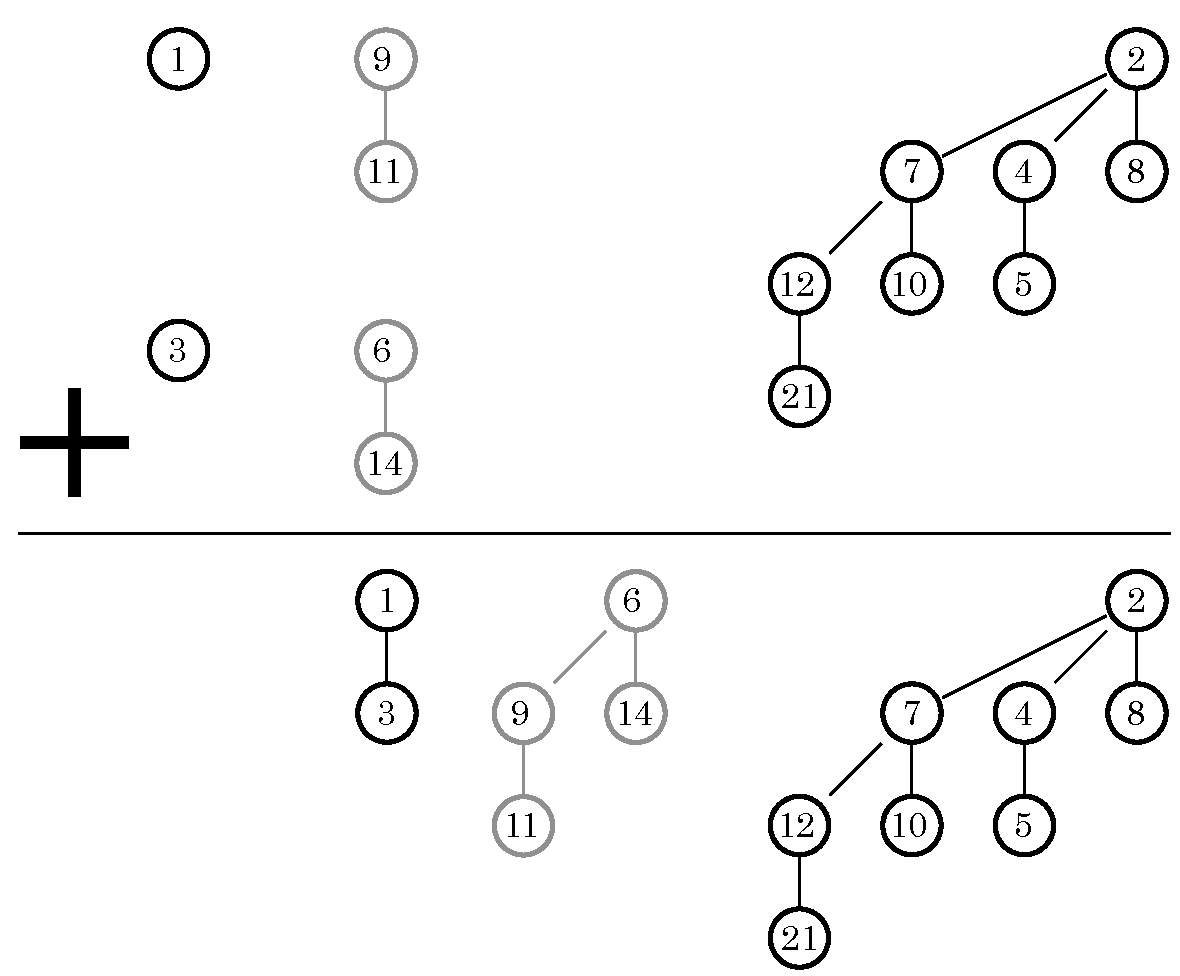
\includegraphics[width=85mm]{spolecne/01/images/Binomial_heap_merge2}
        \caption{Binomiální halda MERGE - 2 příklady}
        \label{fig:binom_heap_add}
    \end{center}
\end{figure}

\begin{table}[ht]
    \centering
    \vspace{0px}
    \begin{tabu}{|[1pt]c|c|c|[1pt]}
        \tabucline[1pt]{-}
        operace & čas. složitost & poznámka \\\tabucline[1pt]{-}
        \texttt{accessMin()} & $\Theta (1)$ &  \textcolor{gray}{přístup k vrcholu haldy} \\\hline
        \texttt{deleteMin()} & $\Theta (\log(n))$ &  \textcolor{gray}{smazání vrcholu haldy} \\\hline
        \texttt{insert(e)} & $\Theta (\log(n))$ amortizovaně: $\Theta(1)$ &  \textcolor{gray}{přidání prvku do haldy} \\\hline
        \texttt{delete(e)} & $\Theta (\log(n))$ &  \textcolor{gray}{smazání elementu haldy} \\\hline
        \texttt{merge(h1,h2)} & $\Theta (\log(n))$ &  \textcolor{gray}{sloučení 2 hald} \\\hline
        \texttt{decreaseKey(k,v)} & $\Theta (\log(n))$ &  \textcolor{gray}{snížení hodnoty klíče $k$ o $v$} \\\hline
    \end{tabu}
    \caption{Binomiální halda - Operace a jejich složitosti}
\label{table:binom_heap_complexity}
\end{table}
\vspace{-10px}
\subsubsection{Fibonacciho halda}
Založena na binomiální haldě. Má relaxovanější strukturu, která umožňuje zlepšené asymptotické složitosti. Fibonacciho halda se nevyužívá v real-time systémech, protože některé operace mají lineární složitost. U operací, které nevyžadují mazání (accesMin, merge, decreaseKey) je amortizovaná složitost $O(1)$.

\paragraph{Struktura.} Fibonacciho haldu tvoří skupina stromů vyhovující lokální podmínce na uspořádání haldy, která vyžaduje, aby pro každý uzel stromu platilo, že prvek, který reprezentuje, je menší než prvek reprezentovaný jeho potomky. Z této podmínky vyplývá, že minimálním prvkem je vždy kořen jednoho ze stromů. Vnitřní struktura Fibonacciho haldy je v porovnání s binomiální haldou daleko více flexibilní. Jednotlivé stromy nemají pevně daný tvar a v extrémním případě může každý prvek haldy tvořit izolovaný strom nebo naopak všechny prvky mohou být součástí jediného stromu hloubky $n$. Tato flexibilní struktura umožňuje velmi jednoduchou implementaci operací s haldou. Operace, které nejsou potřebné, odkládáme a vykonáváme je až v okamžiku, kdy je to nevyhnutelné, například spojení nebo vložení nového prvku se jednoduše provede spojením kořenových seznamů (s konstantní náročností) a jednotlivé stromy spojíme až při operaci snížení hodnoty klíče \cite{wiki:fibonacci}.

\paragraph{Implementace.} Pro rychlé vymazání a zřetězení se vytváří \textit{obousměrný cyklický spojový seznam} kořenů všech stromů (obr. \ref{fig:fibonacci_heap}). Pro potomky každého prvku se vytváří podobný seznam. Pro každý uzel se ukládá počet synů a údaj, zda je zvýrazněn. Navíc si uchováváme ukazatel na kořenový prvek s minimální hodnotou klíče ($MIN$) \cite{wiki:fibonacci}.

\begin{figure}[htbp]
    \begin{center}
        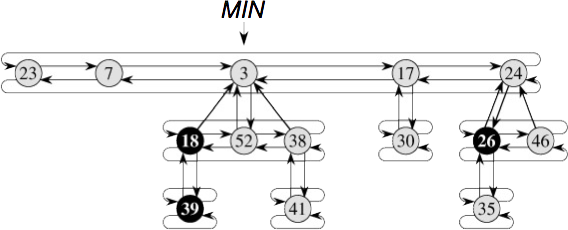
\includegraphics[width=140mm]{spolecne/01/images/fibonacci_heap}
        \caption{Reprezentace fibonacciho haldy}
        \label{fig:fibonacci_heap}
    \end{center}
\end{figure}

\begin{itemize}[itemsep=0px]
\item \textbf{N} - aktuální počet prvků
\item \textbf{MIN} - minimum haldy
\item \textbf{rank} - pomocné pole pří slévání stromů (označení stupně stromů)
\item \textbf{mark(x)} - boolean hodnota indikující jestli prvek x ztratil potomka od té doby kdy x bylo vytvořeno jako potomek jiného prvku. Nově vytvořené prvky jsou neoznačené, a prvek x se stane neoznačeným, vždy když se stane potomkem jiného prvku.
\end{itemize}

\paragraph{Operace.} Operace Fibonacciho haldy a jejich složitosti:

\begin{itemize}[itemsep=0pt, topsep=2pt]
    \item \texttt{accessMin()} - vrátí kořen z Fibonacciho stromu na který ukazuje $MIN$ pointer
    \item \texttt{deleteMin()} - Operace odstranění minima probíhá ve třech krocích. V prvním odstraníme kořenový prvek s minimální hodnotou klíče. Jeho synové vytvoří kořenové prvky nových stromů. Poté se slévají stromy stejného stupně, a nakonec se upraví ukazatel MIN. Při slévání stromů tvořících jednu haldu postupně sjednotíme kořeny stromů stejných stupňů. Uvažujeme, že počet kořenových prvků na počátku operace je N. Pokud máme dva kořeny U a V stejného stupně, vytvoříme z jednoho z nich syna druhého prvku tak, aby kořenovým zůstal prvek s menší hodnotou klíče. Jeho stupeň se pak zvětší o jedničku. Toto opakujeme, dokud v haldě existují dva stromy se stejným stupněm. K efektivnímu hledání stromů stejného stupně používáme pole ukazatelů, ve kterém uchováváme reference vždy na jeden kořen každého stupně. Pokud je nalezen druhý strom stejného stupně, oba stromy jsou spojeny a příslušný ukazatel v poli je aktualizován
    \item \texttt{insert(e)} - vytvoří se nová halda obsahující jediný element \texttt{e}; \texttt{mark(e) = false}; Merge s původní haldou - $O(1)$
    \item \texttt{merge(h1, h2)} - prosté spojení seznamů s kořenovými prvky stromů jednotlivých hald a update $MIN$ pointeru
\end{itemize}

\begin{table}[ht]
    \centering
    \vspace{0px}
    \begin{tabu}{|[1pt]c|c|c|[1pt]}
        \tabucline[1pt]{-}
        operace & čas. složitost & poznámka \\\tabucline[1pt]{-}
        \texttt{accessMin()} & $O(1)$ &  \textcolor{gray}{přístup k vrcholu haldy} \\\hline
        \texttt{deleteMin(e)} & $O(n)$ amortizovaně: $O(\log(n))$ &  \textcolor{gray}{smazání vrcholu haldy} \\\hline
        \texttt{insert(e)} & $O(1)$ &  \textcolor{gray}{přidání prvku do haldy} \\\hline
        \texttt{delete(e)} & $O(n)$ amortizovaně: $O(\log(n))$ &  \textcolor{gray}{smazání elementu haldy} \\\hline
        \texttt{merge(h1,h2)} & $O(1)$ &  \textcolor{gray}{sloučení 2 hald} \\\hline
        \texttt{decreaseKey(k,v)} & $O(\log(n))$ amortizovaně $O(1)$ &  \textcolor{gray}{snížení hodnoty klíče $k$ o $v$} \\\hline
    \end{tabu}
    \caption{Fibonacciho halda - Operace a jejich složitosti}
\label{table:fibo_heap_complexity}
\end{table}
\pagebreak
\paragraph{\texttt{deleteMin()}} Popis operace \texttt{deleteMin} a následné konzolidace haldy.

\lstset{style=php,caption=deleteMin ve Fibonacciho haldě, label=listing:fib_delete}
\begin{lstlisting}[mathescape]
z = MIN;
if (z $\neq$ null) then {
  foreach x $\in$ descendants(z) do
    add $x$ to the root list of the heap;
  remove $z$ from the root list of the heap;
  if (N=1) then {
    MIN = null;
  } else {
    MIN = any pointer to a root from the root list of the heap;
    Consolidate();
  }
  N--;
}
\end{lstlisting}

\lstset{style=php,caption=Konzolidace ve Fibonacciho haldě, label=listing:fib_consol}
\begin{lstlisting}[mathescape]for i = 0 to max. possible degree of a tree in Fibo. heap of size N do A[i] = null;
foreach w $\in$ all trees in the root list of the heap do {
  x = w; d = a degree of the tree w;
  while rank[d] $\neq$ null do {
    y = rank[d];
    if key(x) > key(y) then swap x and y;
    remove y from the root list of the Heap;
    make y a child of x, incrementing the degree of x;
    mark(y) = false; rank[d] = null; d++;
  } 
  rank[d] = x;
}
MIN = null;
for i = 0 to max. degree of a tree in the array A do {
  if rank[i] $\neq$ null then {
    add rank[i] to the root list of the heap;
    If (MIN = null) or (key(A[i]) < key(MIN)) then MIN = A[i];
  }
}
\end{lstlisting}

\begin{table}[ht]
    \centering
    \vspace{0px}
    \begin{tabu}{|[1pt]c|c|c|c|c|[1pt]}
        \tabucline[1pt]{-}
        & \textbf{binary heap} & \textbf{d-ary heap} & \textbf{binomial heap} & \textbf{Fibonacci heap} \\\tabucline[1pt]{-}
         \texttt{accessMin()} & $\Theta (1)$ &  $\Theta (1)$ & $\Theta (1)$ & $\Theta (1)$ \\\hline
        \texttt{deleteMin()} & $\Theta (\log(n))$ & $\Theta (\log(n))$ & $\Theta (\log(n))$ & $O(n);O(\log(n))$ \\\hline
        \texttt{insert(e)} & $\Theta (\log(n))$ & $\Theta (\log(n))$ & $O(\log(n));O(1)$ & $\Theta (1)$ \\\hline
        \texttt{delete(e)} & $\Theta (\log(n))$ & $\Theta (\log(n))$ & $O(\log(n))$ & $O(n); O(\log(n))$ \\\hline
        \texttt{merge(h1,h2)} & $\Theta (n)$ & $\Theta (n)$ & $O (\log(n))$ & $\Theta (1)$ \\\hline
        \texttt{decreaseKey(k,v)} & $\Theta (\log(n))$ & $\Theta (\log(n))$ & $\Theta (\log(n))$ & $O(\log(n)); O(1)$ \\
        \hline
    \end{tabu}
    \caption{Haldy - srovnání složitostí}
\label{table:heaps_complexities}
\end{table}

% https://www.cs.princeton.edu/~wayne/teaching/fibonacci-heap.pdf

\begin{figure}[htbp]
    \begin{center}
        \vspace{-20px}
        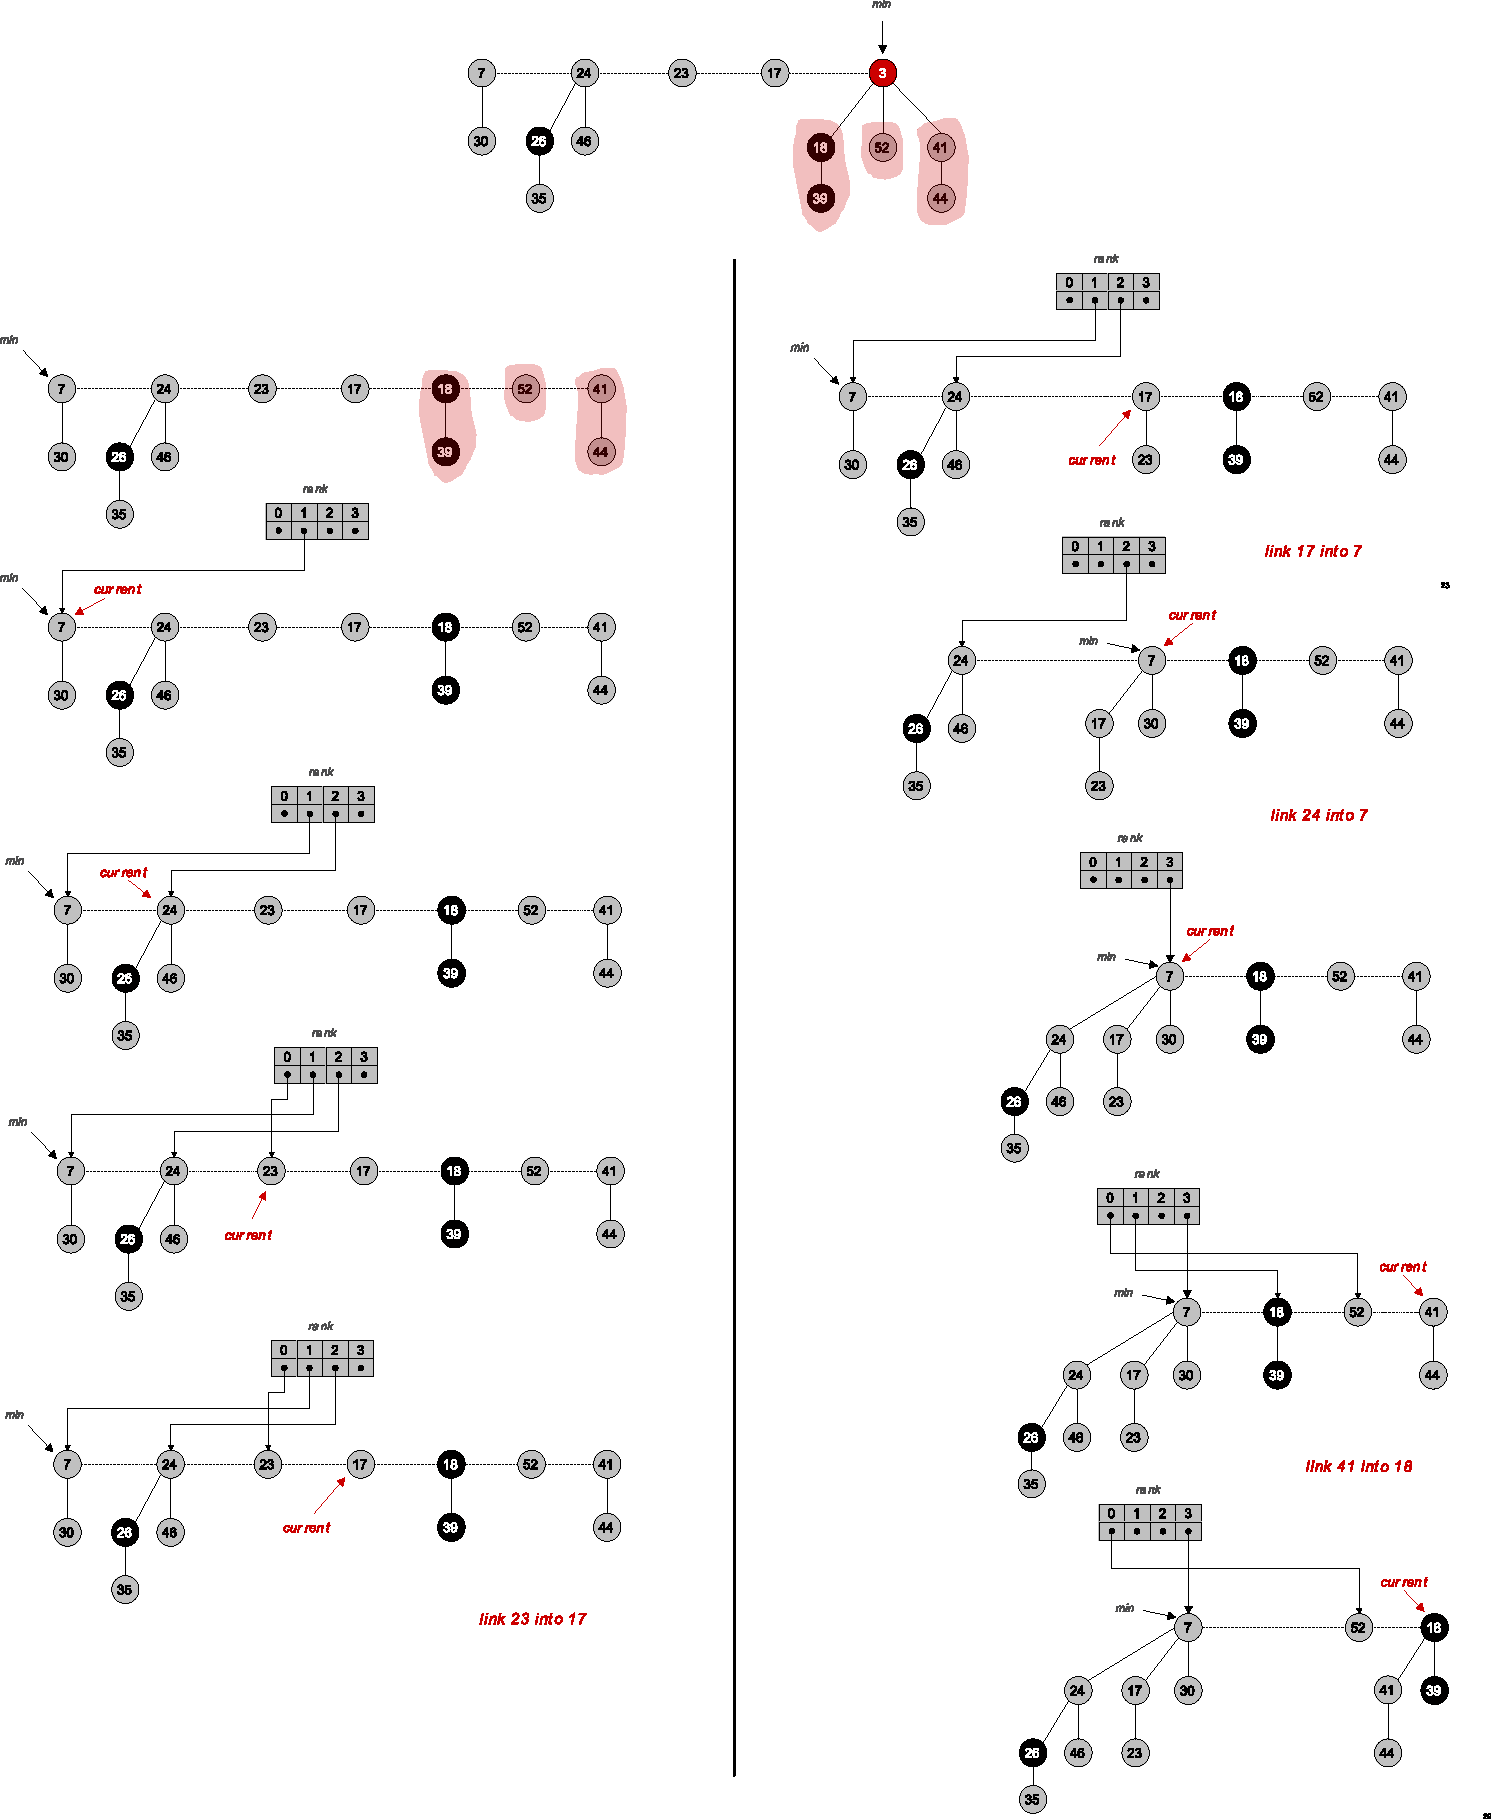
\includegraphics[width=160mm]{spolecne/01/images/fib-heap-del}
        \caption{Postup při deleleMin operaci}
        \label{fig:bin-heap-del}
    \end{center}
\end{figure}

%!TEX root=../oi-magistr-spolecne.tex
\section[PAL - Grafy - refrezentace a algoritmy]{Neorientované a orientované grafy, jejich reprezentace. Prohledávání grafu (do hloubky a do šířky), topologické uspořádání, souvislost, stromy, minimální kostra.}
Graf je uspořádaná dvojice množiny vrcholů a hran $G = (V,E)$. Dá se reprezentovat mnoha způsoby. Nelze říci, který je lepší, protože se každá reprezentace hodí k trochu jinému typu úloh. Nejčastěji je ale graf reprezentován \textbf{maticí sousednosti} (1 kde je hrana), \textbf{laplaceovou maticí} (na diagonále stupeň vrcholu, -1 pro hranu), \textbf{maticí incidence} (řádky jsou body, sloupce hrany, 1 a -1 značí zdrojový a koncový bod) nebo pomocí \textbf{seznamu sousedů} (u každébo bodu list s jeho sousedama).

\paragraph{Silně souvislá komponenta (SCC)}
Graf je silně souvislý jestliže existuje cesta v obou směrech mezi každými dvěma vrcholy. \textbf{SCC} orientovaného grafu je maximální silně souvislý podgraf.

    $$SCC(v) = \{u \in V |~\text{there exists a path in}~G~\text{from}~u~\text{to}~v~\text{and a path in}~G~\text{from}~v~\text{to}~u\}$$
    
\begin{figure}[h]
    \begin{center}
        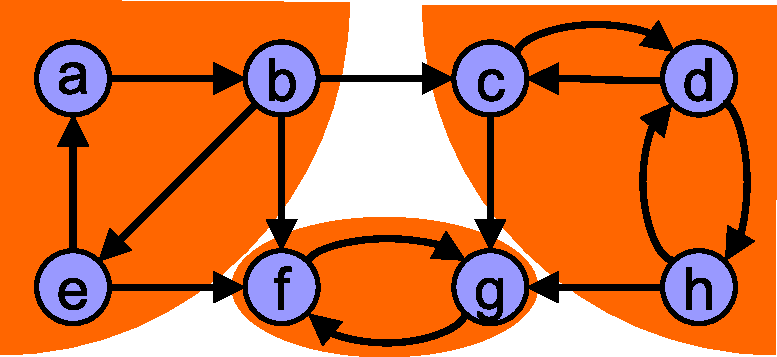
\includegraphics[width=70mm]{02/images/scc}
    \end{center}
\end{figure}

\subsection{Kosaraju}
Používá upravený DFS kde při uzavírání vrcholu ho vloží do stacku $S$. Po prvním průchodu DFS celým grafem prohodí hrany a vyresetuje označení vrcholů. Dokud $S$ obsahuje nějaký vrchol tak ho vybere ze stacku. Pokud vrchol ještě nebyl navštíven tak opět provede DFS. Množina aktuálně navštívených vrcholů dá SCC obsahující i aktuální vrchol.

Algoritmus provádí 2 kompletní průchody grafem. Pokud je graf reprezentován jako list sousedů pak běží v $\Theta(\vert V\vert + \vert E \vert)$, pokud jako matice sousedů tak $O(\vert V^2 \vert)$

\subsection{Tarjan}

Tarjanův algoritmus vychází z prohledávání do hloubky. Vrcholy se při prohledávání indexují dle pořadí svého nalezení. Při návratu z rekurze se každému vrcholu přiřadí uzel s nejnižším indexem na jaký lze dosáhnout. Všechny vrcholy, které mají totožný cílový uzel (index), jsou ve stejné komponentě.

Tarjanův algoritmus má stejně jako prohledávání do hloubky asymptotickou složitost $\Theta(\vert V \vert + \vert E \vert)$ (při použití listu sousedů, jinak při matici sousedů $O(\vert V^2 \vert)$).

\lstset{style=java,caption=Tarjan, label=listing:tarjan}
\begin{lstlisting}
procedure tarjanAlgorithm(Node node, List scc, Stack s, int index)
  v.index = index
  v.lowlink = index
  index++
  s.push(node) //pridej na zasobnik
  for each Node n in Adj(node) do //pro vsechny potomky
    if n.index == -1 //pokud jeste nebyl uzel objeven
      tarjanAlgorithm(n, scc, s, index) //prohledej
      node.lowlink = min(node.lowlink, n.lowlink) //uprav lowlink otce
    else if stack.contains(n) //pokud komponenta nebyla jiz uzavrena
      node.lowlink = min(node.lowlink, n.index)

  if node.lowlink == node.index //pokud jsme v koreni komponenty
    Node n = null
    List component //seznam uzlu dane komponenty
    do
      n = stack.pop() //vyber uzel ze zasobniku
      component.add(n) //pridej ho do komponenty
    while(n != v) //dokud nejsme v koreni
    scc.add(component) //komponentu pridej do seznamu komponent
\end{lstlisting}

\vspace{-15px}

\subsection{Topologické uspořádání}
Topologické uspořádání je taková posloupnost uzlů grafu, že pro každou jeho hranu $(u, v)$ platí, že uzel $u$ je zařazen před uzlem $v$. Topologicky lze proto uspořádat pouze acyklické grafy.

Jinými slovy: Všechny vrcholy grafu G jsou očíslovány tak, že $u\leq v$ platá pro každý pár vrcholů, které mají hranu $(u,v)$

Topologické uspořádání lze zjistit pomocí upraveného DFS. Lze jím testovat grafovou acyklicitu, konektivitu, hledání souvislých komponent.

Algoritmus topologického uspořádání vychází z procházení grafu do hloubky. Jedná se o pořadí uzavření uzlů opačně orientovaného grafu. Časová složitost tohoto postupu proto $O(\vert V \vert + \vert E \vert)$.

\subsection{Minimální kostra grafu - MST}
Kostra grafu G je graf, který má stejný počet vrcholů jako G a je to strom. Minimální kostra grafu je taková kostra, která má součet vah použitých hran nejmenší.

\begin{figure}[h]
    \begin{center}
        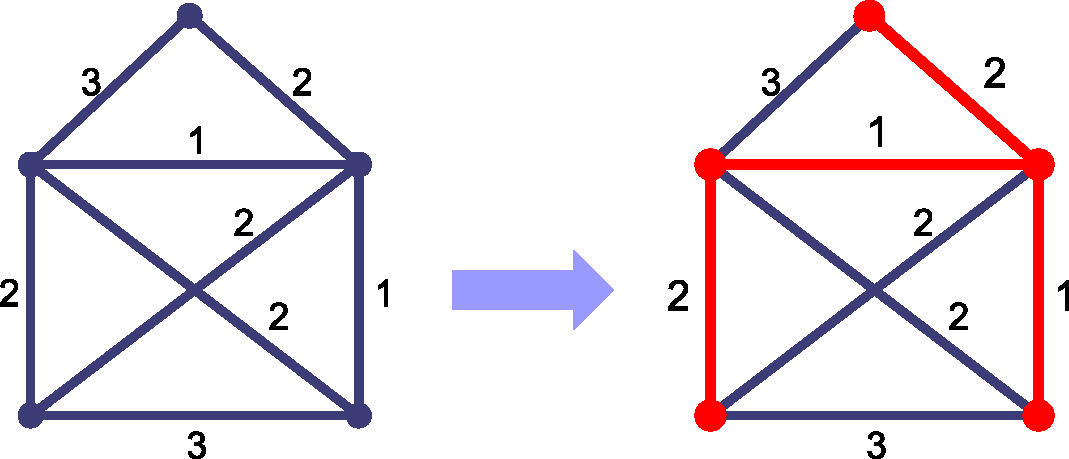
\includegraphics[width=60mm]{02/images/spanning-tree}
    \end{center}
\end{figure}

\vspace{-10px}

\subsubsection{Primův alg.}
Nejprve se vybere libovolný vrchol z $V$ a vloží se do výsledné množiny $K$. K němu se pak v každé iteraci (je jich $V$) hledají takové hrany $(u,v) \in E$, které mají minimální cenu, $u$ je v $K$ a $v$ není v $K$

\begin{algorithm}
\caption{Prim alg.}
\begin{algorithmic}
\State Select an arbitrary vertex $v_0 \in V(G)$
\State $K = \{v_0\}$
\While{$\vert V(K)\vert \neq \vert V(G)\vert$}
  \State Select edge $\{u,v\} \in E(G)$ where $u \in V(K)$ and $v \notin V(K)$ so that $w(\{u,v\})$ is min
  \State $K = K + edge\{u,v\}$
\EndWhile
\end{algorithmic}
\end{algorithm}

\begin{figure}[h]
    \begin{center}
        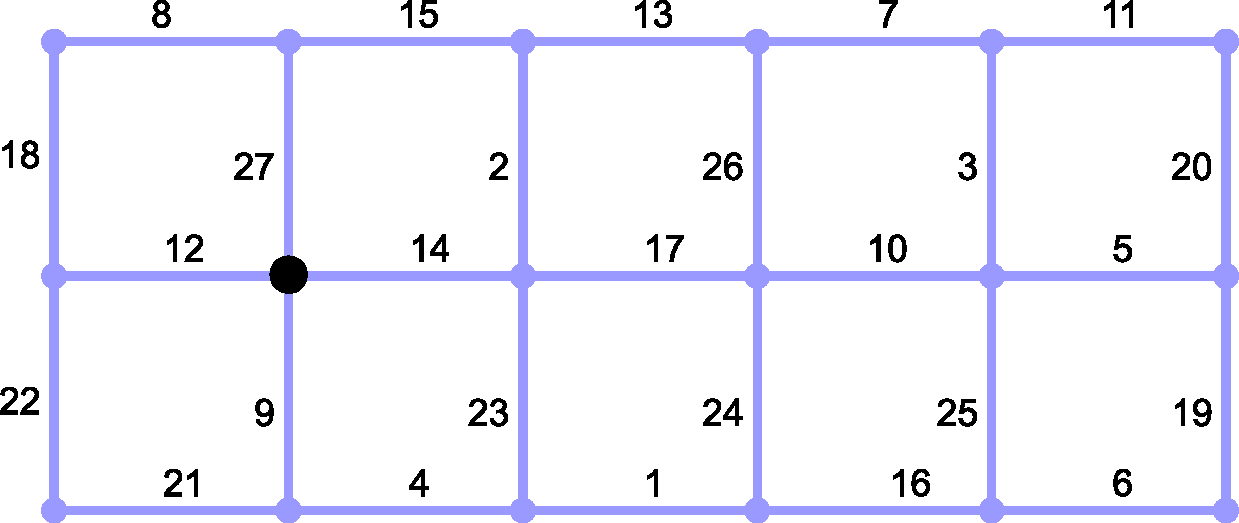
\includegraphics[width=70mm]{02/images/prim01}
        \hspace{10px}
        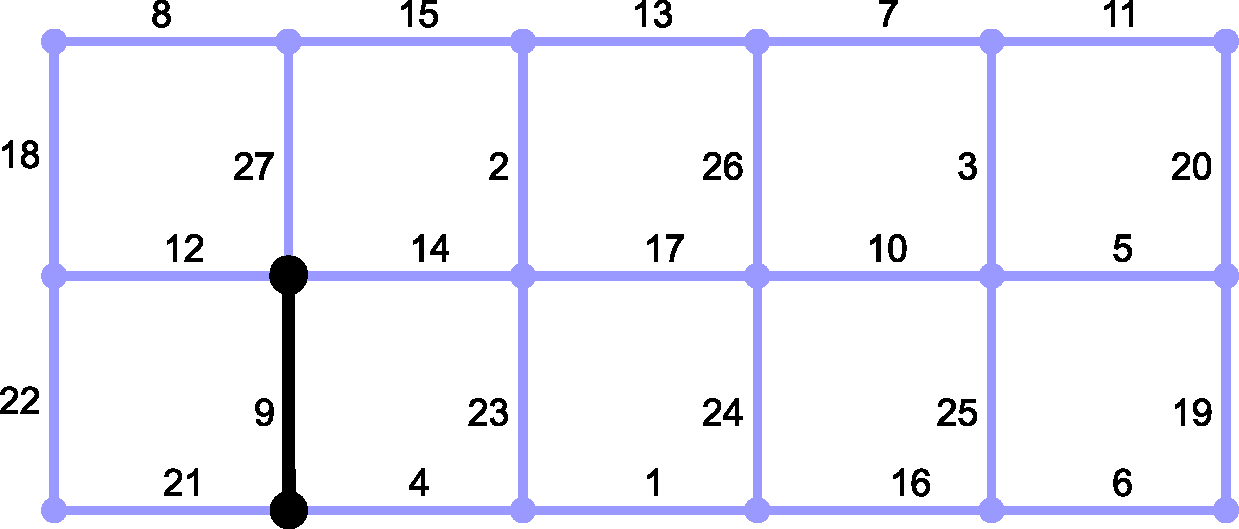
\includegraphics[width=70mm]{02/images/prim02}
    \end{center}
\end{figure}
\vspace{-10px}

Složitost základní implementace je $O(E\cdot V)$. Jednoduchá implementace s použitím reprezentace grafu pomocí matice sousednosti a prohledáváním pole cen má časovou složitost $O(V^2)$. S použitím binární haldy a seznamu sousedů dosáhneme složitosti $O((V + E) \log(V)) = E \log(V)$.


\subsubsection{Borůvkův alg.}
Borůvkův algorimus funguje na principu skládání komponent. Na začátku jsou všechny uzly grafu považovány za samostatné komponenty. Algoritmus v každém svém kroku propojí každou komponentu s jinou komponentou pomocí nejkratší možné hrany. Jelikož Borůvkův algoritmus vyžaduje, aby měly všechny hrany unikátní váhu, tak při propojení komponent nikdy nemůže vzniknout cyklus. Dále je zajištěno, že se v každém kroku zmenší počet komponent minimálně na polovinu - tj. algoritmus terminuje v $\lceil \log_{2} \vert V \vert \rceil$ krocích. Při každém z těchto kroků je třeba najít pro všechny komponenty nejkratší vycházející hranu, což může zabrat až $O(\vert E \vert)$ operací. Celková asymptotická složitost Borůvkova algoritmu je tedy $O(\vert E\vert \cdot \log_{2} \vert V \vert)$.

\begin{algorithm}
\caption{Borůvka alg.}
\begin{algorithmic}
\State $K=(V(G))$
\While{while $K$ has at least two connected components}
  \State For all components $T_i$ of graph $K$ the \textbf{\textit{light incident edge}} $t_i$ is chosen.
  \State All edges $t_i$ are added to $K$
\EndWhile
\end{algorithmic}
\end{algorithm}

\begin{figure}[h]
    \begin{center}
        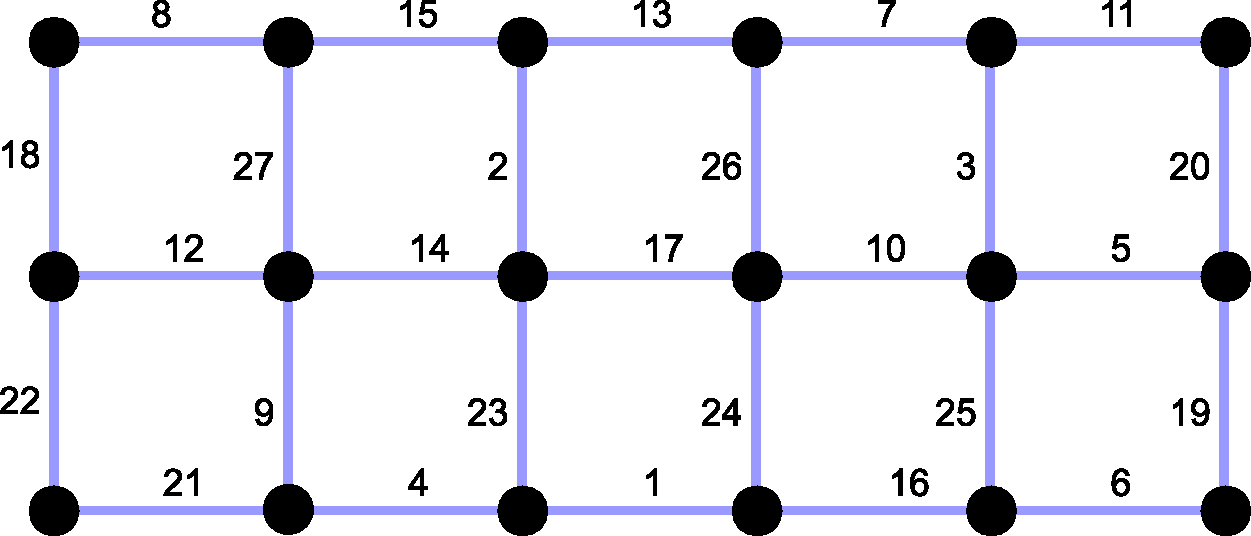
\includegraphics[width=70mm]{02/images/boruvka01}
        \hspace{10px}
        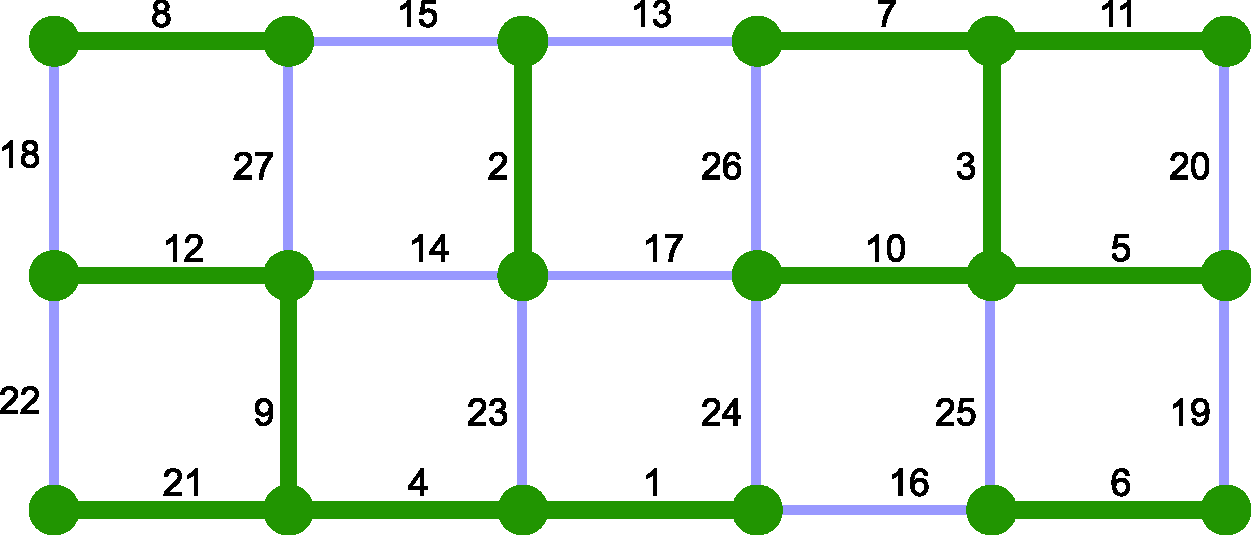
\includegraphics[width=70mm]{02/images/boruvka02}
    \end{center}
\end{figure}

\subsubsection{Kruskalův (\uv{greedy}) alg.}

Kruskalův algoritmus nejprve setřídí hrany dle jejich váhy (od nejmenší) a následně přidává hrany do grafu takovým způsobem, aby nevznikl žádný cyklus (tj. procedura terminuje po přidání $\vert V \vert -1$ hran). V každé iteraci je výsledek podgrafem MST.

K zajištění acykličnosti si algoritmus pomocí datové struktury disjoint set (union-find) udržuje pro každý uzel informaci o příslušnosti ke komponentě souvislosti. Disjoint set poskytuje dvě operace: union (spojí dvě komponenty souvislosti) a find (zjistí pro daný uzel příslušnost ke komponentě souvislosti).

Struktury se ptáme $\vert E(G)\vert$-krát jestli jsou 2 vrcholy ve stejné kmoponentě (operace find) a mergujeme jen $\vert V(G)\vert -1$-krát 2 komponenty do jedné (operace union).

Časová složitost algoritmu je v případě použití řadicího algoritmu založeného na porovnávání $O(\vert E\vert \cdot \log \vert E \vert)$. Pokud jsou hrany již předřazeny, nebo je možno k jejich seřazení použít řadicí algoritmus s lineární složitostí (např. counting sort), tak je složitost Kruskalova algoritmu rovna $O(\vert E\vert \cdot \alpha(\vert E \vert))$, kde $\alpha$ je inverzní Ackermannova funkce (odpovídá složitosti operací union a find).

\begin{algorithm}
\caption{Kruskal alg.}
\begin{algorithmic}
\State Sort all edges $e_1,\dots, e_{m=\vert E(G)\vert} \in E(G)$ so that $w(e_1) \leq \hdots \leq w(e_m)$
\State $K=(V(G))$
\For{$i=1 \hdots m$}
  \If{$K$ + edge $\{u,v\}$ is an acyclic graph}
    \State $K = K$ + edge $\{u,v\}$
  \EndIf
\EndFor
\end{algorithmic}
\end{algorithm}

\begin{figure}[h]
    \begin{center}
        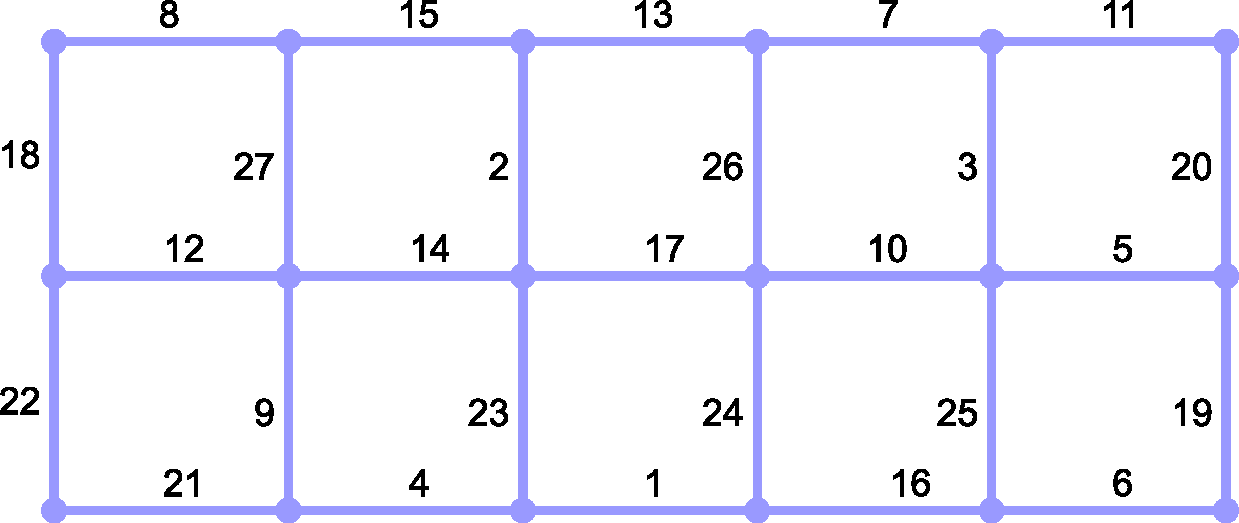
\includegraphics[width=70mm]{02/images/kruskal01}
        \hspace{10px}
        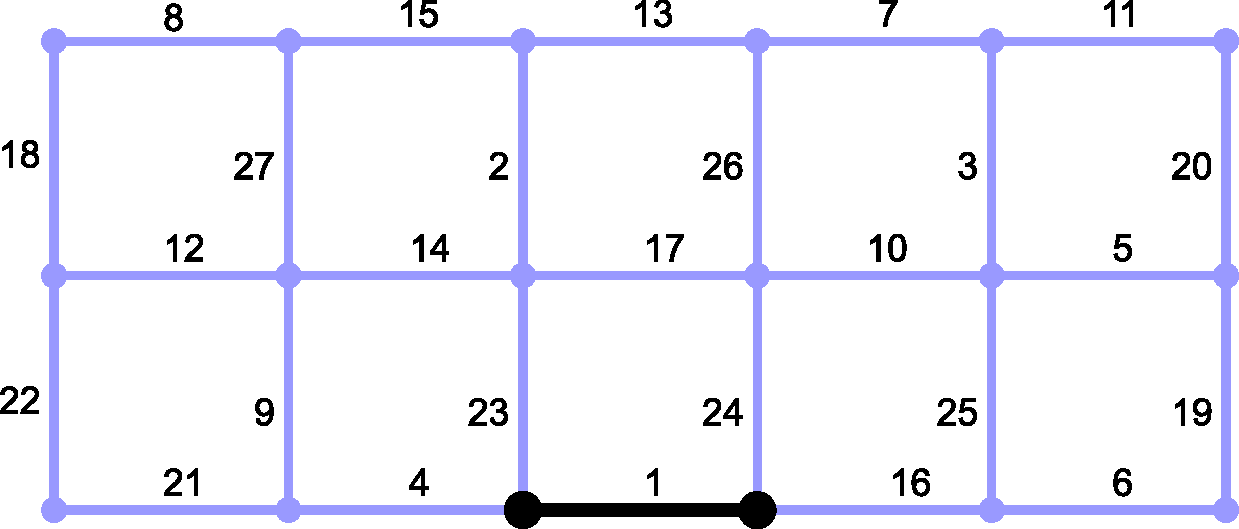
\includegraphics[width=70mm]{02/images/kruskal02}
    \end{center}
\end{figure}

\subsubsection{Union-Find problém}
Problém, který se řeší v kruskalově algoritmu pro hledání MST, při zjišťování, zda 2 vrcholy leží v jedné komponentě, či nikoli - $O(1)$.

\paragraph{Jednoduché řešení} Pole, kde pro každý vrchol udržujem číslo komponenty v jaké je (defaultně obsahuje svoje číslo). Operace find jen vrátí hodnotu na indexu. Union si najde pomocí findu oba prvky a pokud jsou ruzné, tak hodnota jednoho prvků je přepsána na hodnotu druhého (ve všech výskytech) - $O(V)$.

\paragraph{Vylepšené řešení za použití orientovaného stromu}
Ve findu, pokud se naleznou prvky s různými komponentami, tak kořen menšího stromu je přidán jako potomek většího. Hodnoty v poli vždy ukazují na roota komponenty.

\begin{figure}[h]
    \begin{center}
        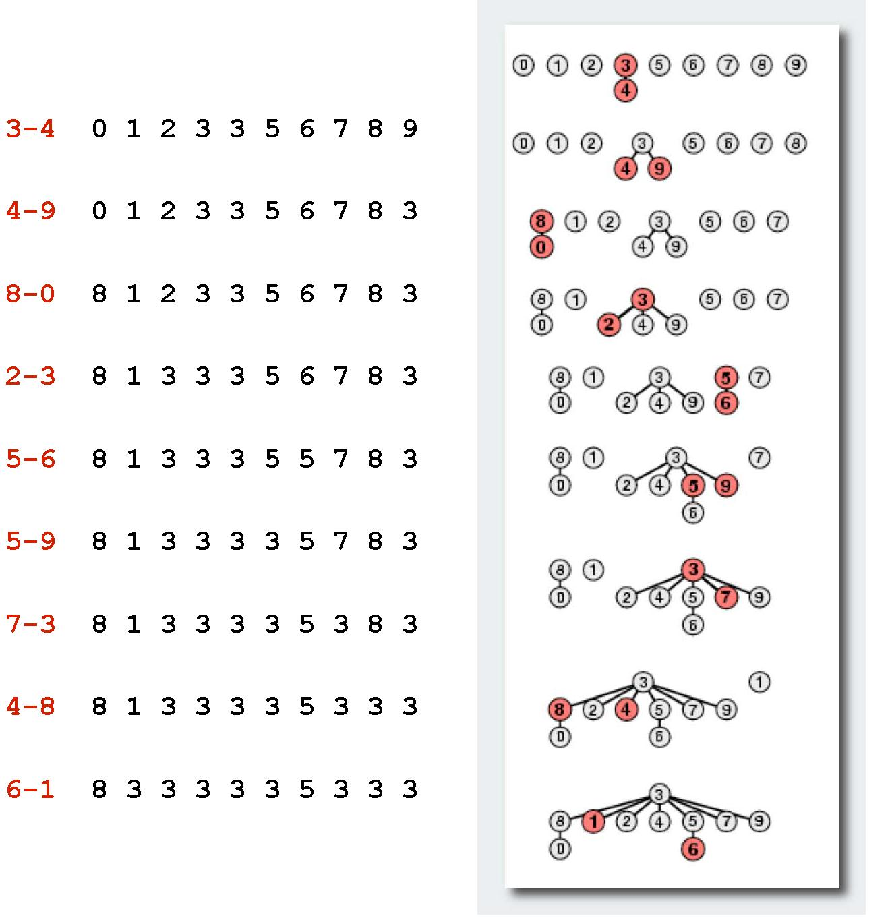
\includegraphics[width=120mm]{02/images/union-find}
    \end{center}
\end{figure}

%!TEX root=../oi-magistr-spolecne.tex
\section[PAL - Stromy]{Vyhledávací stromy: B, B+, R-B, 2-3-4, splay a jejich praktické využití. Problematika vyhledávání ve více dimenzích, K-D stromy.}

Pro vyhledvání se používají naivní metody: sekvenční prohledávání nebo binární půlení pole (předpoklad seřazeného pole), interpolační hledání (seřazené pole).

\subsection{BVS - Binární vyhledávací strom}
Strom, kde uzel má max 2 potomky. Leví potomcí jsou vždy menší, praví větší. Minimum ze stromu je nejlevější prvek (maximum nejpravější).

Hledání, maximum, minimum, následník, předchůdce jsou nalezeny v $O(h)$, kde $h$ je výška stromu. Pokud je strom nevyvážený tak $h=n$ a tedy $O(n)$. Pokud je vyvážený tak $h = \log(n)$ a tím pádem i $O(\log(n))$

\paragraph{Vyvažování stromu} Při různých operacích (např. vložení) by časová náročnost je $O(n)$ kdy je celý strom jedná dlouhá větev. Pro zlepšení složitosti na $O(\log(n))$ se stromy tzv. vyvažují - tím se snižuje počet pater. S tímto pojmem souvísí \textbf{rotace} stromu.

\begin{figure}[h]
    \begin{center}
        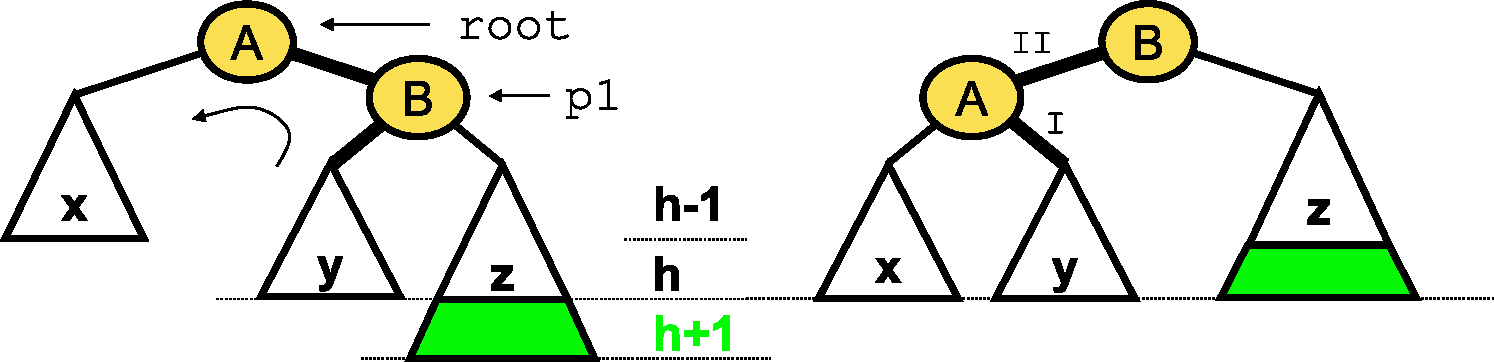
\includegraphics[width=75mm]{spolecne/03/images/rotace-L}
        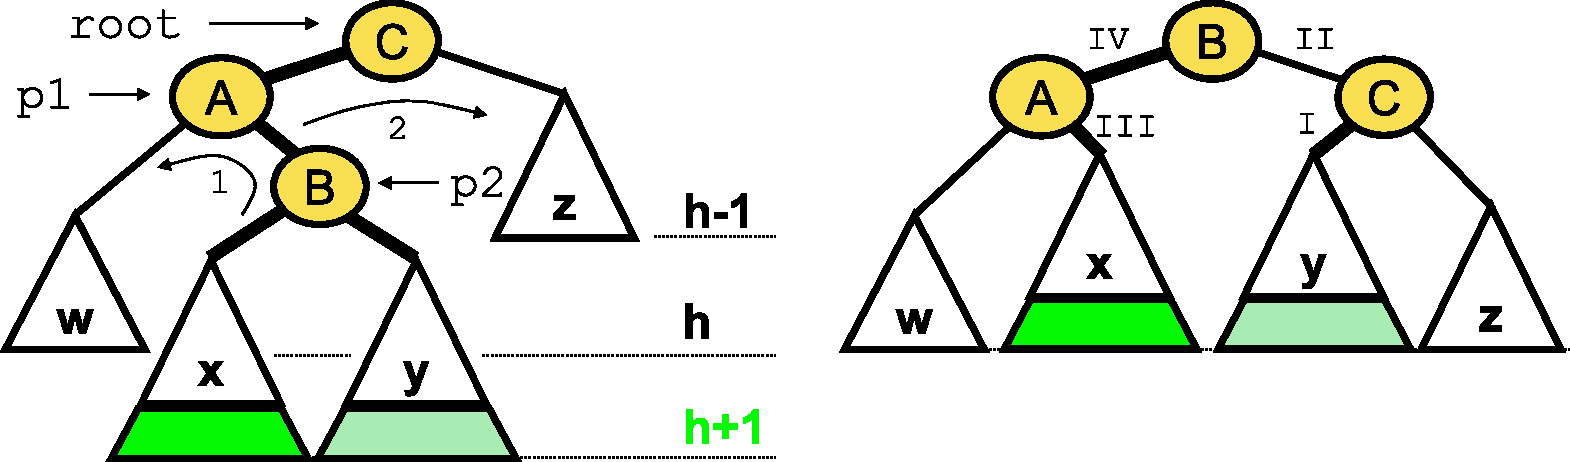
\includegraphics[width=75mm]{spolecne/03/images/rotace-LR}
    \end{center}
    \caption{Levá a levopravá rotace}
\end{figure}

AVL jsou výškově vyvážené stromy.

\subsection{Splay strom}
Splay strom je \textbf{samovyvažující} binární vyhledávací strom mající tu vlastnost, že \textbf{prvky}, k nimž se \textbf{nedávno přistupovalo}, jsou \textbf{rychle} znovu \textbf{dostupné}. Provádí základní operace jako vkládání, vyhledávání a odstraňování prvků v amortizovaném čase $O(\log n)$ (výška je $n$ ale amortizovaně jsou složitosti logaritmické). Výhodou oproti (např. AVL) je, že nepotřebuje udržovat další informaci (výška nebo barva).

Všechny obvyklé operace na binárních vyhledávacích stromech jsou spojeny s jednou základní, které se říká \textit{splay}. Splay uzlu přeuspořádá strom tak, že se daný uzel dostane do kořene. Způsob, jak toho docílit, je provést standardní vyhledávání daného uzlu v binárním stromu a následně provést speciální rotace stromu takové, aby se uzel dostal do kořene. Každý přístup nebo vložení přendá prvek do rootu. \textit{Zig-Zag} a \textit{Zig-Zig} rotace.

\subsection{R-B (Red-Black) strom}
Červeno-černý strom je binární vyhledávací strom. Je vyvážený, jeho hloubka je maximálně dvojnásobek hloubky vyváženého stromu. Jedná se o datovou strukturu často používanou pro implementaci asociativního pole.

Červeno-černý strom musí splňovat následující pravidla:
\begin{itemize}[itemsep=0px]
\item Každý vrchol je buď červený, nebo černý.
\item Kořen je černý.
\item Listy (nil) jsou pokládány za černé vrcholy.
\item Každý červený vrchol má dva černé syny.
\item Každá cesta z jednoho vrcholu do jeho podřízených listů obsahuje stejný počet černých vrcholů.
\end{itemize}

\paragraph{Černá výška} vrcholu \texttt{x} je počet černých vrcholů na cestě z \texttt{x} k listu (nepočítá se vrchol samotný).

\begin{figure}[h]
    \begin{center}
        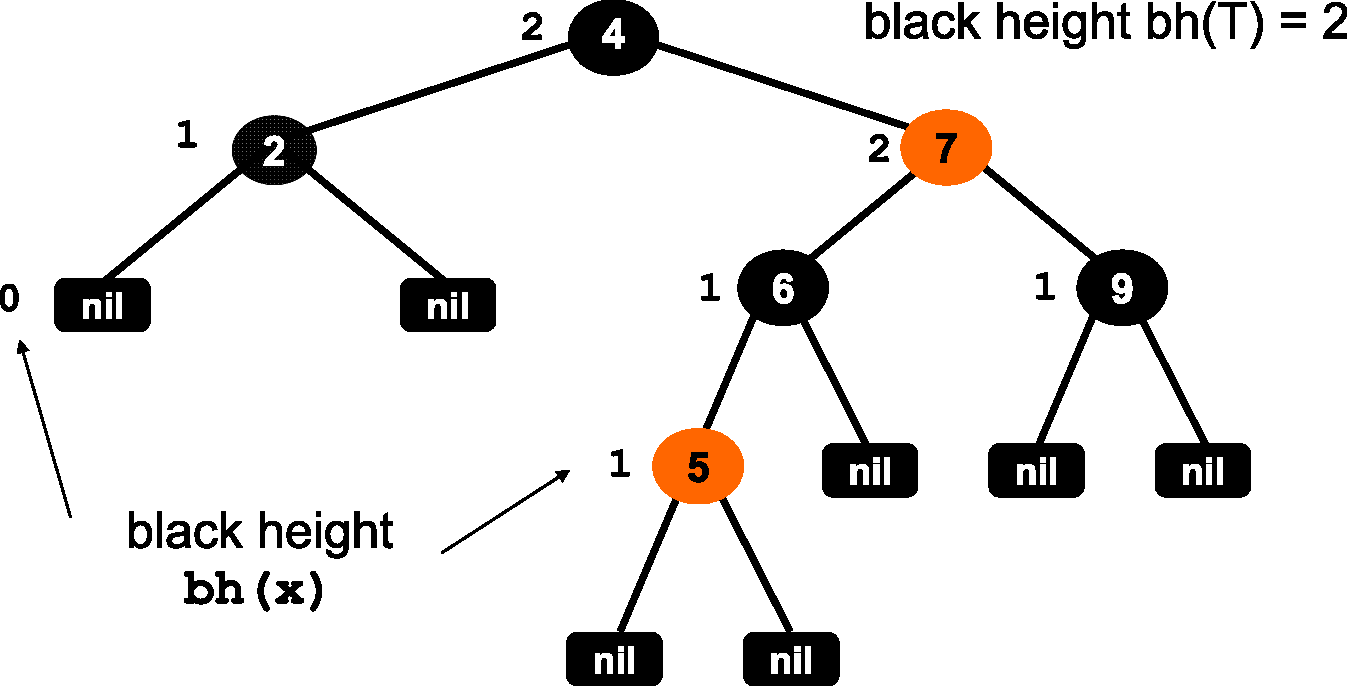
\includegraphics[width=100mm]{spolecne/03/images/red-black}
    \end{center}
\end{figure}

\paragraph{Vkládání $O(\log(n))$ (max 2 rotace)} Nový node \texttt{x} je červený. Vloží se normálně jako v klasickém BST. Pokud je rodič černý, vše je ok. Pokud je rodič červený:

\begin{itemize}
\item jestli je strýc (nodu \texttt{x}) červený - přebarvení
\item jinak jestli je \texttt{x} pravý potomek  - dvojitá rotace (první rotací se z toho stane 3. případ) + přebarvení
\item jinak jednoduchá rotace + přebarvení
\end{itemize}

\paragraph{Mazání $O(\log(n))$ (max 3 rotace)} Najde se vrchol ke smazání a klasicky se smaže (může mít max 1 potomka, jinak ho zaměníme s s nejblížším předchůdcem a pak ho mažem z nové pozice). Pokud je mazaný prvek červený, můžeme ho v klidu smazat - strom stále zůstane R-B.

Nyní předpokládejte, že mazaný prvek je černý a \texttt{X} je označení potomka mazaného (černého) prvku. Pokud je \texttt{X} červený, stačí ho obarvit na černo a tím je konec. Pokud je černý, tak nastávají 4 případy:

\begin{itemize}
\item pokud je sourozenec červený - levá rotace pravého podstromu, přebarvi sourozence a pokračuj do dalšího případu
\item černý sourozenec s 2 černými potomky - obarvi sourozence a jdi (\texttt{X}) nahoru (double černá barva obarví rodiče)
\item černý sourozenec s min 1 červeným potomkem
\begin{itemize}
\item levý potomek je červený - pravá rotace sourozence (transformuje na následující případ)
\item pravý potomek je červený - levá rotace pravého podstromu
\end{itemize}
\end{itemize}


\subsection{B strom}
B-strom je \textbf{zobecněním BST} v tom smyslu, že umožňuje více než 2 potomky. Je specifický tím, že má řád $n$ a limity na maximální ($n$), i minimální ($\left \lceil \frac{n}{2} \right \rceil$) počet potomků vrcholu. B-strom je díky této vlastnosti \textbf{vyvážený}, operace přidání, vyjmutí i vyhledávání tedy probíhají v logaritmickém čase. Tato struktura je často používána v aplikacích, kdy není celá struktura uložena v paměti RAM, ale v nějaké sekundární paměti, jako je pevný disk (například \textbf{databáze}). Protože přístup do tohoto typu paměti je náročný na čas (hlavně vyhledání náhodné položky), snažíme se minimalizovat počet přístupů do této paměti.

B-strom řádu $n$ je takový strom, který splňuje tyto vlastnosti:

\begin{itemize}[itemsep=0px]
\item Všechny listy (tj.uzly které nemají žádné potomky) jsou na stejné úrovni (ve stejné hloubce).
\item Všechny uzly kromě kořene mají maximálně $n$ a minimálně $\left \lceil \frac{n}{2} \right \rceil$ potomků.
\item Kořen má nejvýše n potomků, spodní hranice není omezena.
\end{itemize}

\paragraph{Princip uložení dat}
Data jsou ve stromu uložena jako setříděné hodnoty, které rozdělují strom na jednotlivé podstromy. Například pokud nějaký uzel má tři potomky, musí být v tomto uzlu uloženy dva klíče $k_1$ a $k_2$, které budou uzel rozdělovat. Všechny hodnoty které jsou menší než $k_1$ musí být uloženy v levém podstromu, hodnoty které jsou větší než $k_1$ a menší než $k_2$ musí být uloženy v prostředním podstromu, a konečně všechny hodnoty větší než $k_2$ musí být v pravém podstromu. Na tyto podstromy jsou samozřejmě v uzlu uloženy ukazatele.

List tedy obsahuje $\left \lceil \frac{n}{2} \right \rceil -1$ až $n-1$ klíčů a neobsahuje žádný ukazatel na podstrom. Vnitřní uzel (tj. takový uzel, který není listem ani kořenem) obsahuje stejný počet klíčů $k$, ale tyto klíče rozdělují potomky tohoto uzlu do $k+1$ podstromů.
Kořen má maximálně $n-1$ klíčů a nemusí mít žádné potomky - v tom případě je pak zároveň listem.

Pokud chceme vložit nebo smazat data (klíče) z uzlu, změní se tím počet potomků tohoto uzlu. Aby se dodržel rozsah daný řádem stromu, vnitřní uzly se v případě potřeby rozdělují či slučují.

\paragraph{Vkládání} Multi vs single fáze strategie vkládání

\begin{figure}[h]
    \begin{center}
        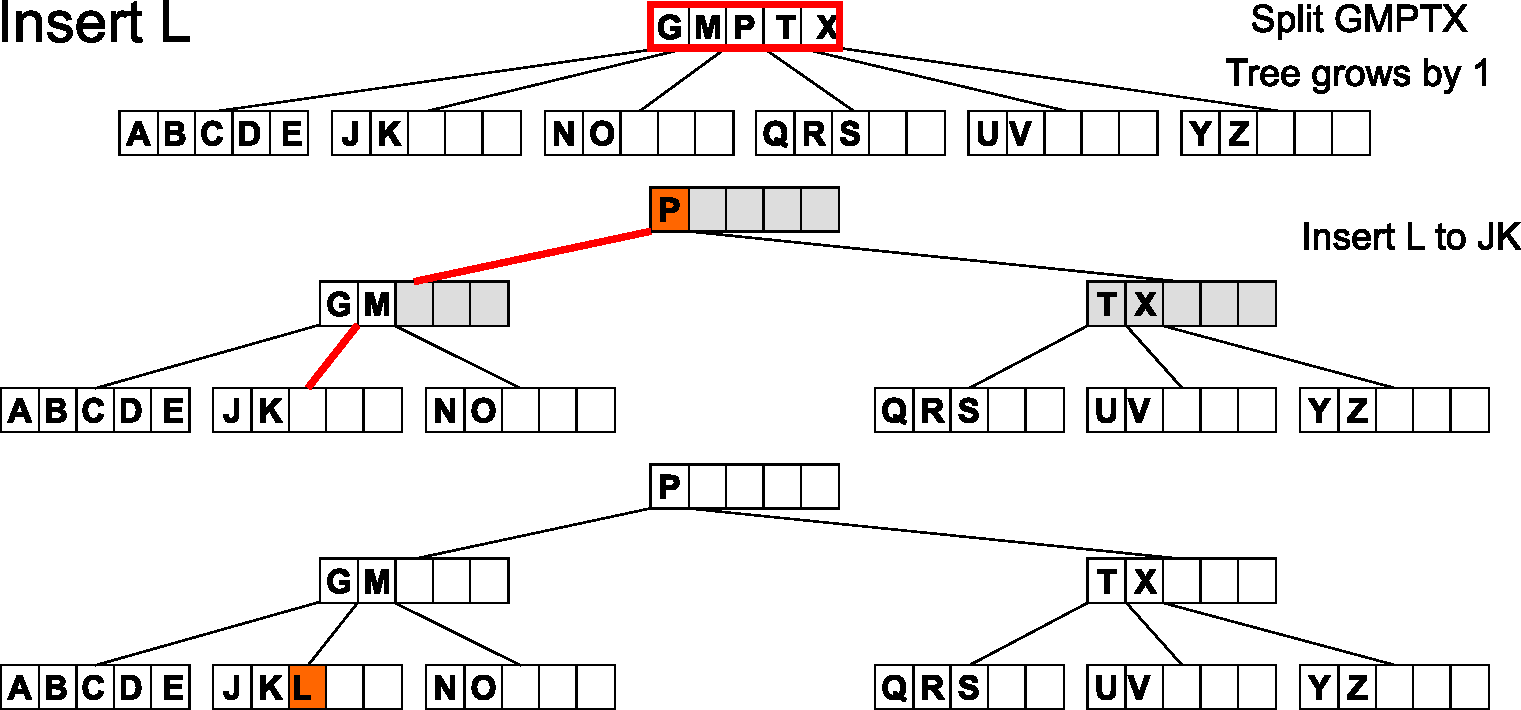
\includegraphics[width=130mm]{spolecne/03/images/btree-insert}
    \end{center}
    \caption{singlephase strategie vkládání (\uv{avoid the future problems})}
\end{figure}

\paragraph{Mazání} jen multipass strategie!

\begin{figure}[h]
    \begin{center}
        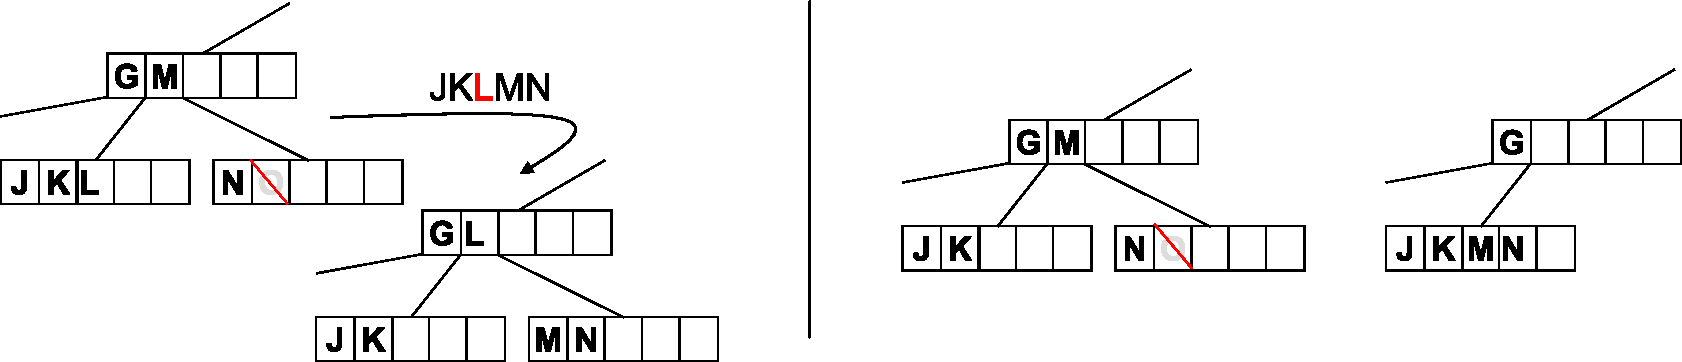
\includegraphics[width=140mm]{spolecne/03/images/btree-delete}
    \end{center}
\end{figure}

\subsection{2-3-4 strom}
2-3-4 vyhledávací strom je buď prázdný nebo obsahuje 3 typy prvků:

\begin{itemize}
\item \textbf{2}-nody s jedním klíčem, levým odkazem na strom s menšími klíči a pravým odkazem na strom s většími klíči.
\item \textbf{3}-nody s dvěma klíči, levým odkazem na strom s menšími klíči, prostředním odkazem na strom s hodnotami mezi a pravým odkazem na strom s většími klíči.
\item \textbf{4}-nody s třemi klíči a čtyřmi odkazy na stromy s klíči s hodnotami mezi.
\end{itemize}

Všechny odkazy na prázdné stromy (např. listy) mají stejnou vzdálenost od kořene - strom je \textbf{perfektně vyvážený}. Vkládání (s mírným vylepšením) a mazání je stejné jako v B-stromu.

\textbf{2-3-4 strom je strukturou stejný jako B-strom řádu 4.}

\begin{figure}[h]
    \begin{center}
        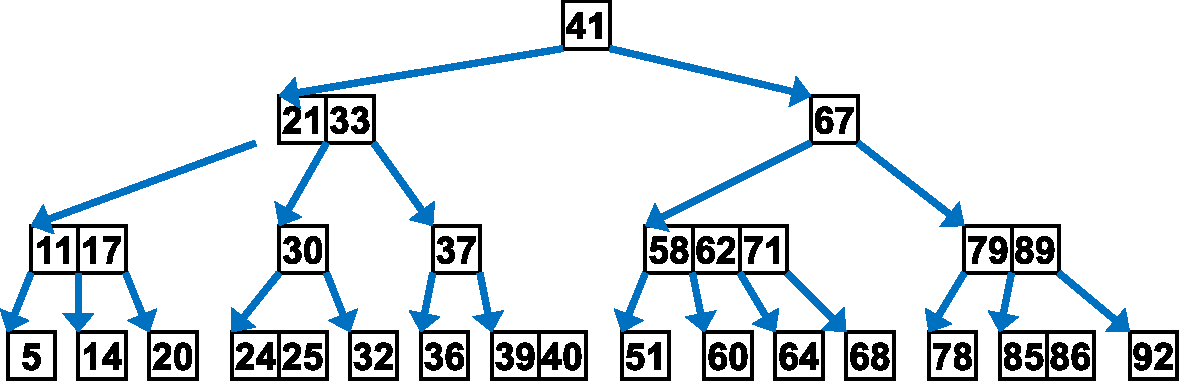
\includegraphics[width=130mm]{spolecne/03/images/234tree}
    \end{center}
\end{figure}

\subsection{B+ strom}
\textbf{Podobný B-stromu (vždy perfektně vyvážený)} s rozdíly: \textbf{Hodnoty} jsou uloženy \textbf{jen v listech}. Interní prvky obsahují jen vyhledávací klíče a jsou použity jen jako placeholdery k nasměrování hledání.

Listy jsou spolu linkovány ve formě LinkedListu. Hodnoty pak mohou být získány sekvenčně bez přístupu skrze strom.

\begin{figure}[h]
    \begin{center}
        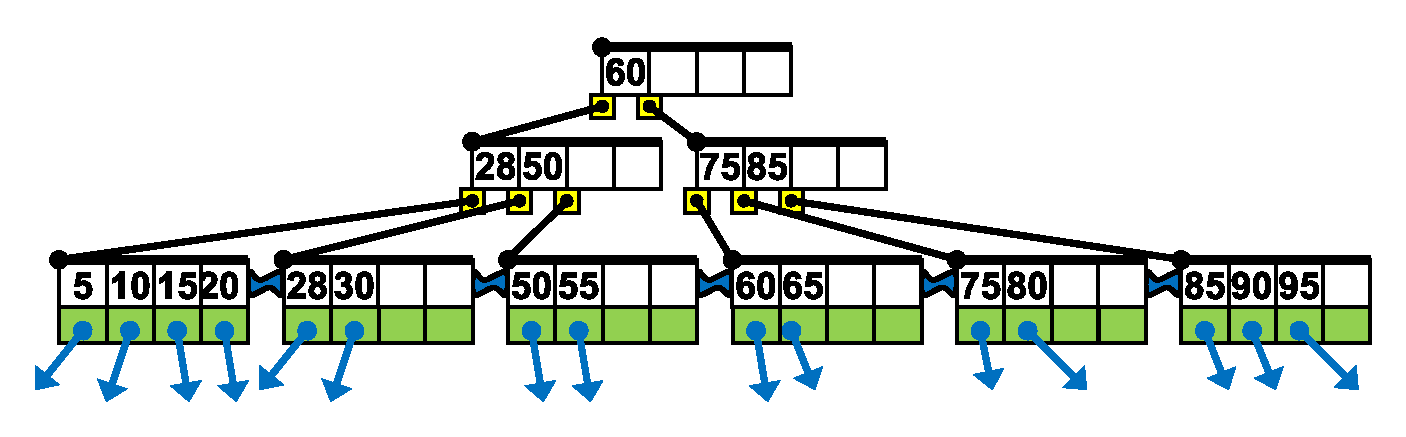
\includegraphics[width=130mm]{spolecne/03/images/bplustree}
    \end{center}
\end{figure}

Find, Insert, Delete - $\Theta(\log_b n)$ - $b$ je řád stromu, $n$ je počet prvků


\subsection{Vyhledávání ve více dimenzích}

\subsection{K-D strom}
Je BVS reprezentující obdélníkovou plochu v D-dimenzionálním prostoru. Plocha je rozdělena (a rekurzivně dorozdělena) do obdélníkových buněk. Dimenze jsou značeny podle jejich indexu $0,1,\hdots,D-1$.

$R$ je kořen stromu (nebo podstromu). Obdélníková D-dimenzionální buňka $C(R)$ (hyperobdelník) je asociován s $R$. Jsou definovány souřadnice $R[0],R[1], ..$ a hloubka stromu $h$.

\begin{figure}[h]
    \begin{center}
        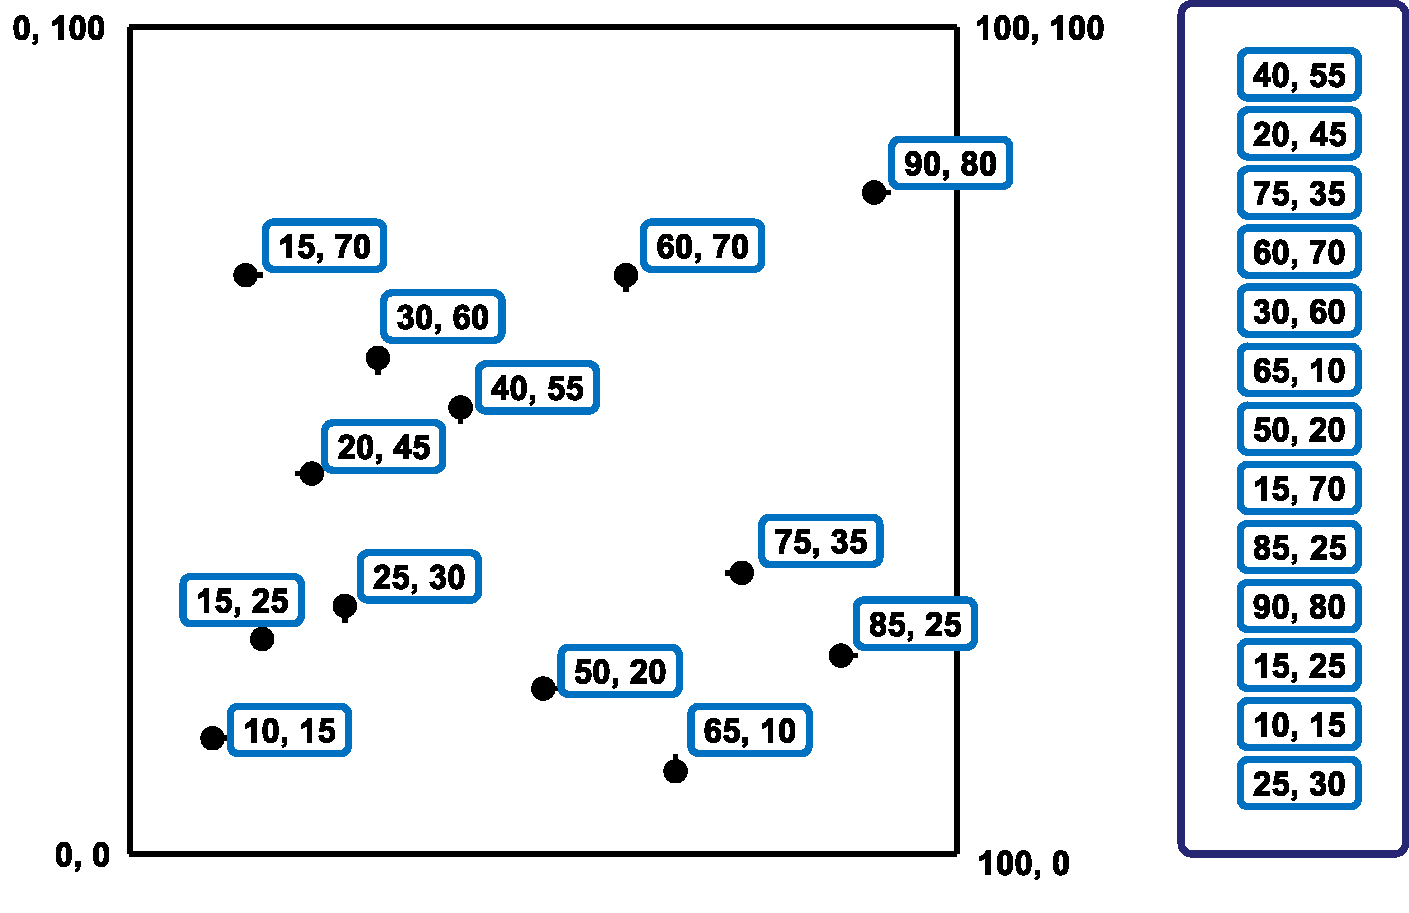
\includegraphics[width=130mm]{spolecne/03/images/kdtree01}
        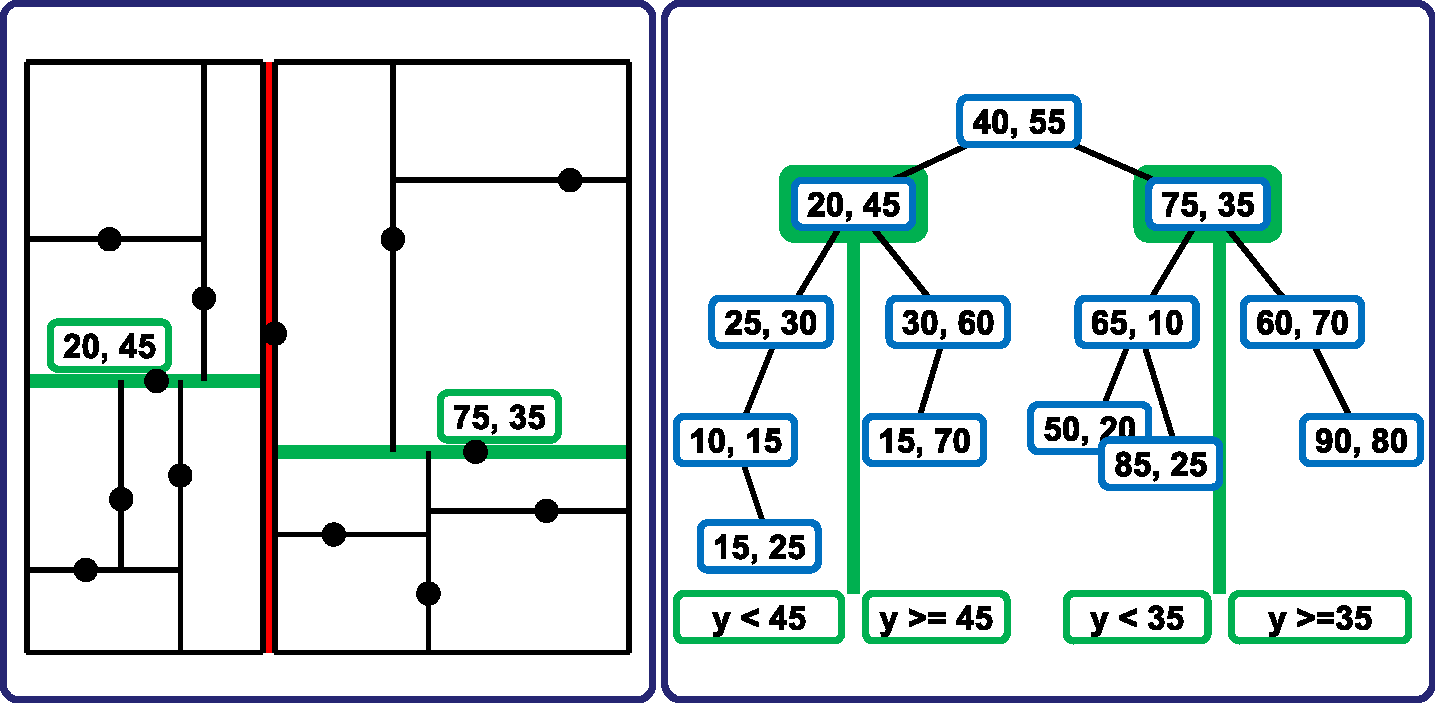
\includegraphics[width=130mm]{spolecne/03/images/kdtree02}
    \end{center}
\end{figure}

\paragraph{Operace}
\begin{itemize}
\item \textbf{Find(key)} - stejné jako v 1D stromě. Hledá se střídavě podle souřadníc odpovídající hloubce stromu (modulo) a postupně se osekává vyhledávaný prostor.

\item \textbf{Insert(key)} - stejné jako v 1D stromě. Porovnávají se střídavě souřadníce odpovídající hloubce stromu (modulo) a postupně se projde až k listu, kam se nový prvek vloží.

\item \textbf{FindMin(dim)} - minimální prvek pro určitou dimenzi. Tato operace je provedena jako část operace delete. Nejnáročnější operace (protože delete metoda rapidně mění strukturu stromu) - $O(n^{1-1/d})$.

\item \textbf{Delete()} - jen listy mohou být smazány. Mazání prvku uvnitř stromu je zajištěno náhradou hodnot, za hodnoty jiného odpovídajícího prvku hlouběji ve stromu. Pokud pravý podstrom R není prázdný, najdi v něm minimum (podle dimenze hledaného prvku). Pokud je prázdný hledej v levém podstromu (podle dimenze hledaného prvku).
\end{itemize}

\subsection{Skip List}
Je seřazený linkedlist kde každý prvek obsahuje proměnný počet odkazů. $k$-tý link implementuje jednoduchý linkedlist, který přeskakuje prvky s menším počtem linků než $k$.

Je to LinkedList s vyhledávací náročnosti $O(\log(n))$. Problém má navazujícími insert/delete operacemi - ty ničí \uv{správný} tvar listu a tím. Řešením je vytvořit náhodný tvar podobný tomu optimálnímu, malé náhodné deviace v dlouhém běhu využití struktury nám tolik nevadí.

\begin{itemize}
\item \textbf{find} - postupně se prochází top-level listy a postupně se míří níže.
\item \textbf{insert} - opět se postupně prochází níže až se vloží nový prvek a náhodně se vygeneruje $k$ pro nově vzniklý prvek - doplní se linky na ostatní prvky.
\end{itemize}

\begin{figure}[h]
    \begin{center}
        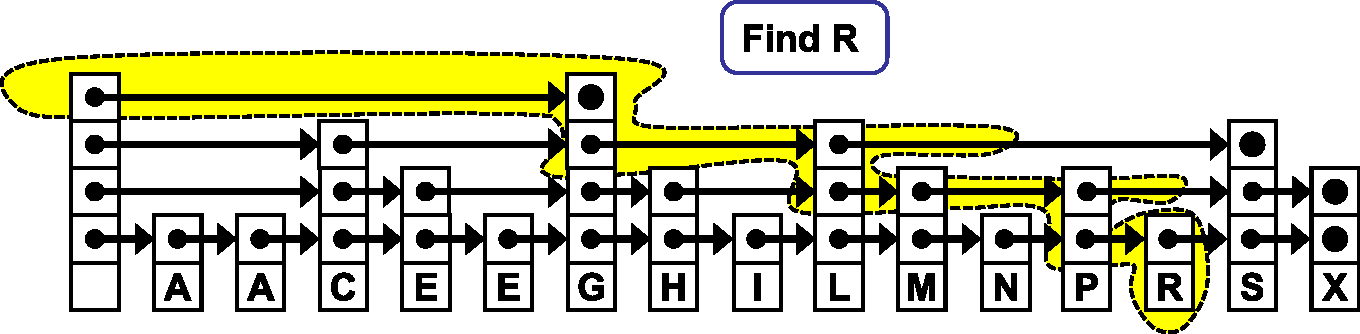
\includegraphics[width=130mm]{spolecne/03/images/skiplist}
    \end{center}
\end{figure}
%!TEX root=../oi-magistr-spolecne.tex
\section[PAL - Vyhledávání v textu, automaty]{Přesné a přibližné hledání množin vzorků v textu, Hammingova a Levenshteinova vzdálenost. Efektivní algoritmy hledání založené na využití konečných automatů. Klasické hledání v textu (naivní, Boyer-Moore). Slovníkové automaty.}

\begin{itemize}
\item \textbf{Abeceda:} Konečná množina znaků. Značí se $A$
\item \textbf{Text:} Posloupnost znaků nad danou abecedou. Symboly textu se značí $t_1, \hdots, t_n$
\item \textbf{Vzorek:} Posloupnost znaků nad stejnou abecedou, jejich výskyt se hledá v daném textu. Text bývá řádově delší než vzorek. Symboly vzorku se značí $p_1, \hdots, p_m$
\end{itemize}

\subsection{Hammingova vzdálenost}
Hammingova vzdálenost $k \geq 0$, je minimální číslo takové, že změnou symbolů na $k$ různých pozicích v jednom z řetězců získáme druhý řetězec. Symboly nelze vypouštět nebo přidávat, Hammingova vzdálenost je \textbf{definována} jen pro \textbf{řetězce stejné délky}. V praxi se implementuje pomocí dynamického programování podobně jako Levenshteinova vzdálenost. Využití při vyhledávání podřetězců.

\begin{figure}[h]
    \begin{center}
        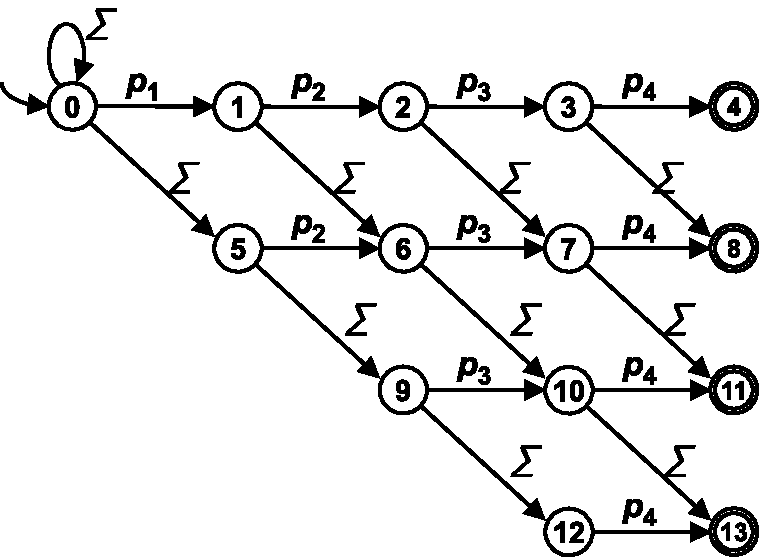
\includegraphics[width=60mm]{04/images/hamming-automat}
    \end{center}
    \caption{NFA, který přijímá slovo s Hammingovou vzdáleností max 3 od vzoru $p_1p_2p_3p_4$}
\end{figure}

\subsection{Levenshteinova vzdálenost}
Levenshteinova vzdálenost je minimální počet operací \textbf{vkládání, mazání a substituce} takových, aby po jejich provedení byly zadané řetězce totožné. Používá se dynamické programování (předpočítaná tabulka).

\paragraph{Vyplnění tabulky:}

\begin{enumerate}
\item v nultém řádku a sloupcy tabulky $A$ jsou postupně inkrementované čísla od 0
\item pokud jsou znaky na pozici $(i,j)$ shodné, vložíme na pozici $(i,j)$ hodnotu $A(i-1, j-1)$
\item pokud se znaky liší, na pozici $(i,j)$ vložíme minimum z těchto tří hodnot:
\begin{enumerate}
\item $A(i,j-1)+1$ - odpovídá operaci odstranění znaku
\item $A(i-1,j)+1$ - odpovídá operaci vložení znaku
\item $A(i-1,j-1)+1$ - odpovídá operaci substituce znaku
\end{enumerate}
\item Výsledky najdeme v posledním řádku tabulky. Zajímají nás sloupce, kde je hodnota menší rovna požadované Levenshteinově vzdálenosti. Čteme zprava doleva.
\end{enumerate}


\begin{table}[h]
\begin{tabular}{|l|l|l|l|l|l|l|l|l|l|}
\hline
           &   & \textbf{S} & \textbf{a} & \textbf{t} & \textbf{u} & \textbf{r} & \textbf{d} & \textbf{a} & \textbf{y} \\ \hline
           & 0 & 1          & 2          & 3          & 4          & 5          & 6          & 7          & 8          \\ \hline
\textbf{S} & 1 & \textbf{0} & \textbf{1} & \textbf{2} & 3          & 4          & 5          & 6          & 7          \\ \hline
\textbf{u} & 2 & 1          & 1          & 2          & \textbf{2} & 3          & 4          & 5          & 6          \\ \hline
\textbf{n} & 3 & 2          & 2          & 2          & 3          & \textbf{3} & 4          & 5          & 6          \\ \hline
\textbf{d} & 4 & 3          & 3          & 3          & 3          & 4          & \textbf{3} & 4          & 5          \\ \hline
\textbf{a} & 5 & 4          & 3          & 4          & 4          & 4          & 4          & \textbf{3} & 4          \\ \hline
\textbf{y} & 6 & 5          & 4          & 4          & 5          & 5          & 5          & 4          & \textbf{3} \\ \hline
\end{tabular}
\vspace{15px}
\caption{Levenshteinova vzdálenost slova \uv{Sunday} a \uv{Saturday} = 3}
\end{table}

\subsection{Hledání v textu pomocí konečných automatů}

\paragraph{Deterministický konečný automat (DFA)} je automat, který z každého stavu může přejít do maximálně jednoho cílového stavu.

\paragraph{Nedeterministický konečný automat (NFA)} je automat, který z každého stavu může přejít do libovolného počtu cílových stavů. Po přečtení jednoho symbolu ze vstupu přejde současně do všech cílových stavů a ze všech těchto stavů pokračuje čtením dalšího vstupu. V přechodové tabulce NKA je navíc sloupeček pro prázdný vstup, označovaný $\epsilon$ (prázdné slovo; $\epsilon~\sum$). Epsilon-přechody automat provádí neustále bez čtení symbolu ze vstupu.

DFA i NFA jsou definovány jako pětice ${A, Q, q_0, F, \delta}$, kde $A$ je vstupní konečná abeceda, $Q$ je množina vnitřních stavů, $q_0$ je počáteční, $F$ je neprázdná množina koncových stavů, $\delta$ je přechodová funkce.

\paragraph{Přechodová funkce:}
\begin{itemize}
\item V DFA je $\delta : Q \times A \rightarrow Q$
\item V NFA je $\delta : Q \times A \rightarrow P(Q)$, kde $P$ je potenční množina
\end{itemize}

\begin{figure}[h]
    \begin{center}
        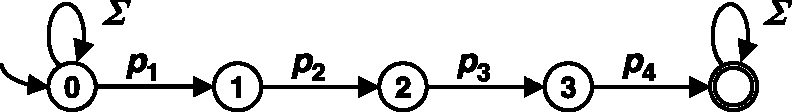
\includegraphics[width=100mm]{04/images/automat-hledani}
    \end{center}
    \caption{NFA, který přijímá jakékoliv slovo se substringem $p_1p_2p_3p_4$ (kdekoliv)}
\end{figure}

\paragraph{Převod NFA do DFA} Opisuju všechny stavy + přidávám nově vzniklé \uv{multistavy}. Tabulka může narůst až na $2^n$ stavů.

\paragraph{Operace s automaty:} S tím souvisí $\epsilon$-přechod. To je takový přechod, který se děje neustále, bez přečtení vstupu.
\begin{itemize}
\item \textbf{union} - vytvoří se nový start stav a do obou start stavů sjednocovaných automatů se vytvoří $\epsilon$-přechod
\item \textbf{concatenation} - z finálních stavů A se vytvoří $\epsilon$-přechody do start stavů B
\item \textbf{iteration} - nový start stav s $\epsilon$-přechodem do startu A; z finálních stavů A $\epsilon$-přechody do startů A.
\item \textbf{intersection} - kartézský součin stavů z obou automatů
\end{itemize}

\subsection{Naivní hledání}
\begin{enumerate}
\item Přiložíme vzorek k začátku textu.
\item Dokud znaky vzorku a textu souhlasí, posunujeme se ve vzorku kupředu.
\item Když narazíme na neshodu, posuneme celý vzorek o jednu pozici kupředu, ve vzorku se nastavíme na začátek a jdeme na 2.
\item Když dojdeme za konec vzorku nebo vzorek přesáhne za konec textu, ohlásíme výsledek a případně postupujeme dále jako ve 3.
\end{enumerate}

Složitost tohoto postupu je $O(m \cdot n)$, kde $m$ je délka vzoru a $n$ je délka textu.

\subsection{Boyer-Moore}
\begin{enumerate}
\item Vzorek přiložíme k textu a testujeme shodu vzorku odzadu.
\item Když dojde k neshodě, je šance, že vzorek lze posunout o více pozic dopředu, mnohdy o celou délku vzorku. Čím delší vzorek, tím rychlejší hledání!
\end{enumerate}
\paragraph{Kolize na poslední pozici vzorku}
Dopomáhá nám tabulka BCS (bad character shift). BCS je tabulka indexovaná znaky abecedy značící vzdálenost znaků od konce vzorku. Když tam znak není, je vzdálenost délka vzorku.

\begin{figure}[h]
    \begin{center}
        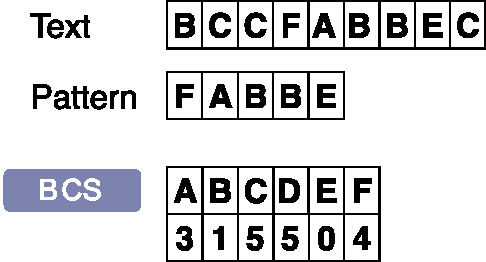
\includegraphics[width=50mm]{04/images/bcs}
    \end{center}
\end{figure}

\paragraph{Kolize po částečné shodě na konci vzorku} Nastávají 3 případy:

\begin{itemize}
\item Přípona $p$ se ve vzorku vyskytuje, a to tak, že jí předchází jiný znak než právě ve vzorku kolidující. Pak musíme vzorek posunout tak, aby se tato další nejbližší instance přípony kryla s textem, tj. o vzdálenost mezi těmito instancemi přípony.
\item Některá přípona vzorku stejně dlouhá nebo kratší než $p$ se vyskytuje také na začátku vzorku. Uvažme nejdelší takovou příponu, označme její výskyt na začátku vzorku symbolem $q$. Vzorek pak musíme posunout o vzdálenost mezi $p$ a $q$.
\end{itemize}

Tabulka GSS (Good Suffix Shift) obsahuje přípony vzorku všech možných délek od 1 do $m$, kde $m$ je délka vzorku a k těmto příponám počet pozic, o které se má vzorek posunout v případě kolize.

\begin{figure}[h]
    \begin{center}
        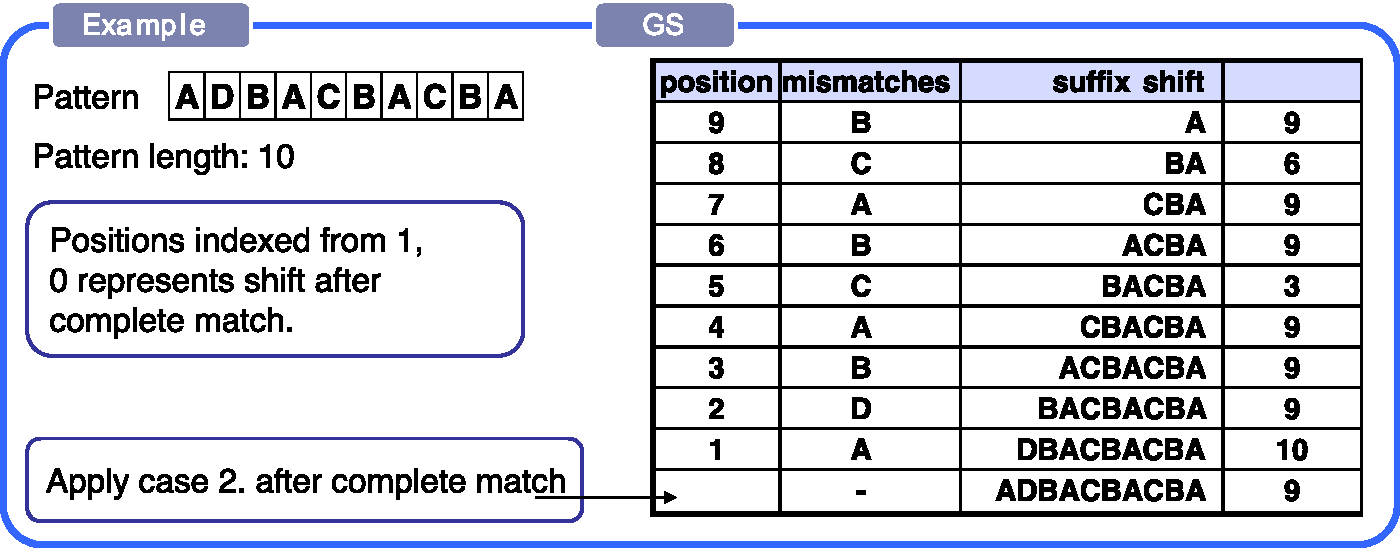
\includegraphics[width=120mm]{04/images/gss}
    \end{center}
\end{figure}


\subsection{Slovníkové automaty}
Slovník nad abecedou A je konečná množina řetězců (patternů) z A*. Slovníkový automat hledá text pro jakýkoliv řetězec ve slovníku.

\begin{itemize}
\item Abeceda: A = \{a, c, d, e, g, h, i, l, m, n, o, q, r, s, t, u, v, y\}
\item Slovník: D = \{add, advanced, algorithms, to, your, algonqiuan, adventures\}
\end{itemize}

Stejné prefixy se dají mergovat do společných stavů.

\begin{figure}[h]
    \begin{center}
        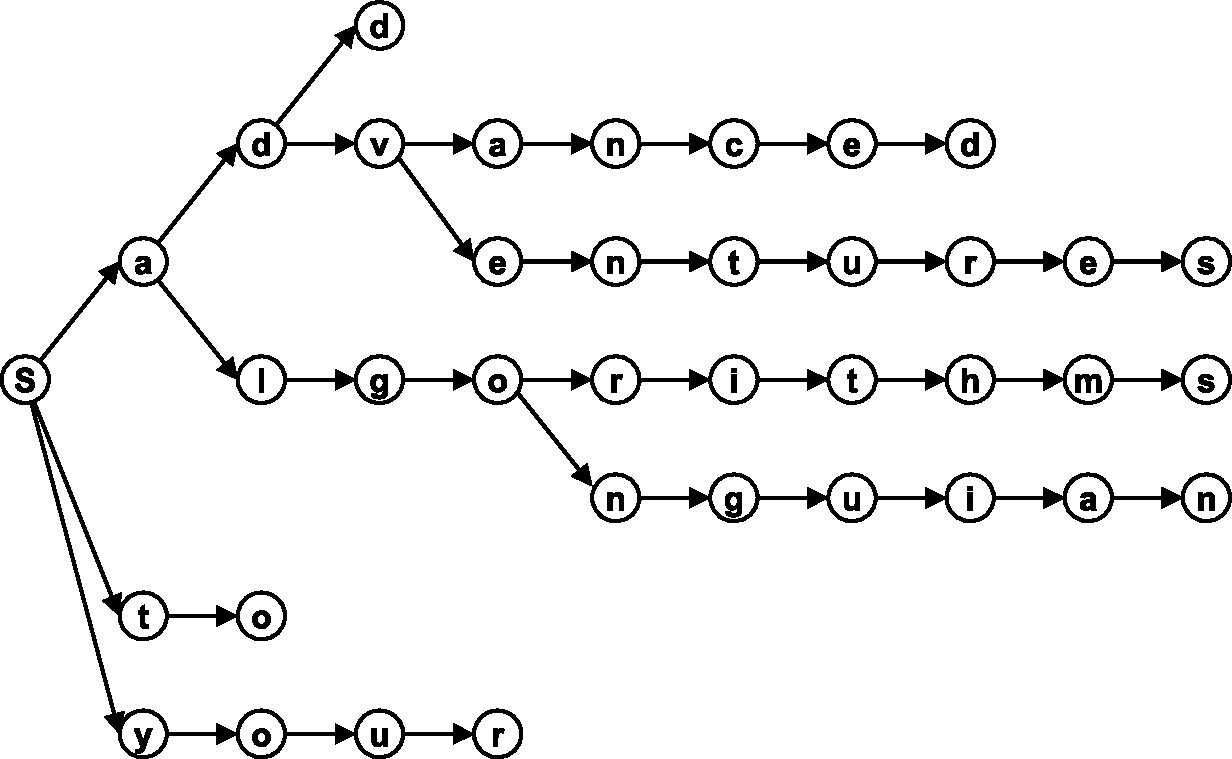
\includegraphics[width=120mm]{04/images/slovnikovy-automat}
    \end{center}
    \caption{Slovníkový automat (bez suffix vylepšení)}
\end{figure}

\paragraph{Vylepšení:} Identické suffixy lze mergovat do jednoho stavu, např. \uv{add} - lze zrušit jeden stav (koncové \uv{d}) a dát přechod do jiného koncového \uv{d} (např. u slova \uv{advanced}).
%!TEX root=../oi-magistr-spolecne.tex
\section[TAL - Algoritmus, $\mathcal{P}$, $\mathcal{NP}$]{Algoritmus, správnost algoritmu, složitost algoritmu, složitost úlohy, třída $\mathcal{P}$, třída $\mathcal{NP}$.}

\paragraph{Algoritmus.}
\label{algoritmus}
\textit{Algoritmem} rozumíme dobře definovaný proces, tj. posloupnost výpočetních kroků, který přijímá hodnoty (zadání, vstup) a vytváří hodnoty (řešení, výstup).

Řekneme, že algoritmus $\mathcal{A}$ \textit{řeší}  úlohu $\mathcal{U}$, jestliže pro každý vstup (každou instanci problému $\mathcal{U}$) vydá správné řešení.

\paragraph{Správnost algoritmu}
K ověření správnosti algoritmu je třeba ověřit 2 věci:
\begin{enumerate}[itemsep=0pt]
    \item algoritmus se na každém vstupu zastaví
    \item algoritmus po zastavení vydá správný výstup - řešení
\end{enumerate}

\paragraph{Variant}
Důkaz faktu, že se algoritmus na každém vstupu zastaví, je založen na nalezení tzv. \textit{variantu}. Variant je hodnota udaná přirozeným číslem, která se během práce algoritmu snižuje až nabude nejmenší možnou hodnotu (a tím zaručuje ukončení algoritmu po konečně mnoha krocích).

\paragraph{Invariant}
\textit{Invariant}, též \textit{podmíněná správnost algoritmu}, je tvrzení, které:
\begin{itemize}[itemsep=0pt]
    \item platí před vykonáním prvního cyklu algoritmu, nebo po prvním vykonání cyklu
    \item platí-li před vykonáním cyklu, platí i po jeho vykonání
    \item při ukončení práce algoritmu zaručuje správnost řešení
\end{itemize}

\subsection{Složitost algoritmu}
Složitost algoritmu udává, jak je daný algoritmus rychlý (kolik provede elementárních operací) vzhledem k množině vstupních dat. Ke klasifikaci algoritmů se obvykle používá tzv. asymtotická složitost, což je rozdělení algoritmů do tříd složitostí, u kterých platí, že od určité velikosti dat, je algoritmus dané třídy vždy pomalejší než algoritmus třídy předchozí, bez ohledu na to, jestli je některý z počítačů $c$-násobně výkonnější ($c$ je konstanta).

Algoritmy lze rozdělit do několika tříd složitosti na základě času a paměti, jež potřebují ke svému vykonání na různých typech Turingových strojů. \cite{algoritmy:slozitosti}

Časovou složitost algoritmu udáváme jako asymptotický odhad $T(n)$ času potřebného pro vyřešení každé instance velikosti $n$.

\subsubsection{Asymptotický růst funkcí} Definujeme několik symbolů (množin).

\paragraph{Symbol $\mathcal{O}$.} Je dána nezáporná funkce $g(n)$. Řekneme, že nezáporná funkce $f(n)$ je $\mathcal{O}(g(n))$, jestliže existuje kladná konstanta $c$ a přirozené číslo $n_0$ tak, že

\begin{center}
    $f(n) \leq c \cdot g(n)$ pro všechny $n \geq n_0$
\end{center}

$\mathcal{O}(g(n))$ můžeme též chápat jako třídu všech nezáporných funkcí $f(n)$:

\begin{center}
    $\mathcal{O}(g(n)) = \{ f(n)~|~\exists c > 0, n_o$ tak, že $f(n) \leq c \cdot g(n) ~ \forall n \geq n_0\}$
\end{center}
\noindent Další symboly:
\begin{itemize}[itemsep=0pt]
    \item $\Omega(g(n)) = \{ f(n)~|~\exists c > 0 ,n_o$ tak, že $f(n) \geq c \cdot g(n) ~ \forall n \geq n_0\}$
    \item $\Theta(g(n)) = \{ f(n)~|~\exists c_1,c_2 > 0 ,n_o$ tak, že $c_1 \cdot g(n) \leq f(n) \leq c_2 \cdot g(n) ~ \forall n \geq n_0\}$
    \item $o(g(n)) = \{ f(n)~|~\forall c > 0 ~\exists n_o$ tak, že $ 0 \leq f(n) < c \cdot g(n) ~ \forall n \geq n_0\}$
    \item $\omega(g(n)) = \{ f(n)~|~\forall c > 0 ~\exists n_o$ tak, že $ 0 \leq c \cdot g(n) < f(n) ~ \forall n \geq n_0\}$
\end{itemize}

\paragraph{Tranzitivita $\mathcal{O}, \Omega, \Theta$.} Máme dány tři nezáporné funkce $f(n), g(n), h(n)$
\begin{itemize}[itemsep=0pt]
    \item Jestliže $f(n) \in \mathcal{O}(g(n))$ a $g(n) \in \mathcal{O}(h(n))$, pak $f(n) \in \mathcal{O}(h(n))$
    \item Jestliže $f(n) \in \Omega(g(n))$ a $g(n) \in \Omega(h(n))$, pak $f(n) \in \Omega(h(n))$
    \item Jestliže $f(n) \in \Theta(g(n))$ a $g(n) \in \Theta(h(n))$, pak $f(n) \in \Theta(h(n))$
\end{itemize}

\paragraph{Reflexivita $\mathcal{O}, \Omega, \Theta$.} Pro všechny nezáporné funkce $f(n)$ platí:
\begin{itemize}[itemsep=0pt]
    \item $f(n) \in \mathcal{O}(f(n))$
    \item $f(n) \in \Omega(f(n))$
    \item $f(n) \in \Theta(f(n))$
\end{itemize}

\subsubsection{Master Theorem}
\label{heading:mastertheorem}
Používá se pro určení asymptotického časového odhadu u rekurentních vztahů.

\noindent
Jsou dána přirozená čísla $a \geq 1, b \geq 1$ a funkce $f(n)$. Předpokládejme, že funkce $T(n)$ je dána na přirozených číslech rekurentním vztahem

\begin{center}
    $T(n)=aT\left(\frac{n}{b}\right)+f(n),$ kde $\frac{n}{b}$ znamená buď $\lfloor \frac{n}{b} \rfloor$ nebo $\lceil \frac{n}{b} \rceil$.
\end{center}

\begin{enumerate}[itemsep=0pt]
    \item Jesltiže $f(n) \in \mathcal{O}(n^{\log_ba - \epsilon})$ pro nějakou konstantu $\epsilon > 0$, pak $T(n) \in \Theta(n^{\log_ba})$.
    
    \item Jesltiže $f(n) \in \Theta(n^{\log_ba})$, pak $T(n) \in \Theta(n^{\log_ba} \lg n)$.
    
    \item Jesltiže $f(n) \in \Omega(n^{\log_ba + \epsilon})$ pro nějakou konstantu $\epsilon > 0$ a jestliže $a f(\frac{n}{b}) \leq c f(n)$ pro nějakou konstantu $c < 1$ pro všechna dostatečně velká $n$, pak $T(n) \in \Theta(f(n))$.
\end{enumerate}

\noindent MT nepokrývá všechny případy.

\newpage

\example{Příklad}{
    \begin{spacing}{1.4}
        \noindent $T(n) = 6T\left(\frac{n}{4}\right) + n^2.\lg(n)$ \textcolor{gray}{// 3. případ $n^2\lg(n) \in \Omega(n^{\log_46})$} \\
        $6 \left(\frac{n}{4}\right)^2 \lg\left(\frac{n}{4}\right) \leq c \cdot n^2 \lg(n)$ \textcolor{gray}{// roznásobení} \\
        $\frac{6}{16} n^2 \lg\left(\frac{n}{4}\right) \leq c \cdot n^2 \lg(n)$ \textcolor{gray}{// $\lg\left(\frac{n}{4}\right)$ si "zvětším" na $\lg(n)$} \\
        $\frac{6}{16} n^2 \lg(n) \leq c \cdot n^2 \lg(n)$ \textcolor{gray}{// pokrátím (vydělím) $n^2 \lg(n)$} \\
        $\frac{6}{16} \leq c$ \textcolor{gray}{// $c < 1$, platí} \\
        $\rightarrow T(n) = \Theta(n^2 \lg(n))$
    \end{spacing}
}

\subsubsection{Řešení rekurzivních vztahů pomocí rekurzivních stromů}

\example{Příklad}{
    \begin{spacing}{1}
        \Tree 
        [.{$T(n) = 3T\left(\frac{n}{4}\right) + n^2$} 
            [.{$T\left(\frac{n}{4}\right)$} 
                    {.} 
                    {.} 
                    {.} 
                ] 
            [.{$T\left(\frac{n}{4}\right)$} 
                [.{$T\left(\frac{n}{16}\right)$} 
                    {.} 
                    {.} 
                    {.} 
                ] 
                [.{$T\left(\frac{n}{16}\right)$} 
                    {.} 
                    {.} 
                    {.} 
                ] 
                [.{$T\left(\frac{n}{16}\right)$} 
                    {.} 
                    {.} 
                    {.} 
                ] 
            ] 
            [.{$T\left(\frac{n}{4}\right)$} 
                    {.} 
                    {.} 
                    {.} 
                ]
        ]
        
    \end{spacing}
    \vspace{10px}
    \noindent Vytvoříme si jednotlivé hladiny stromu, který popisuje rekurzivní výpočet funkce $T(n)$. V nulté hladině máme pouze $T(n)$ a hodnotu $n^2$, kterou potřebujeme k výpočtu $T(n)$ (známe-li $T\left(\frac{n}{4}\right)$.
        V první hladině se nám výpočet $T(n)$ rozpadl na tři výpočty $T(n)$. K tomu potřebujeme hodnotu $3 \cdot (\frac{n}{4})^2 = \frac{3}{16} n^2$.
        Při přechodu z hladiny $i$ do hladiny $i + 1$ se každý vrchol rozdělí na tři a každý přispěje do celkové hodnoty jednou šestnáctinou předchozího. Proto je součet v hladině $i$ roven $(\frac{3}{16})^i n^2$.
        Poslední hladina má vrcholy označené hodnotami $T(1)$ a tím rekurze končí. Počet hladin odpovídá $\log_4 n$. V poslední hladině je $3^{\log_4 n} = n^{\log_4 3}$ hodnot $T(1)$. Proto platí
    
    $$T(n) = \sum\limits_{i = 0}^{\log_4 n} \left(\frac{3}{16}\right)^i n^2 + \Theta(n^{\log_4 3})$$
    
    \noindent Odtud
    
        $$T(n) < n^2 \sum\limits_{i = 0}^{\infty} \left(\frac{3}{16}\right)^i + \Theta(n^{\log_4 3}) = n^2 \frac{1}{1 - \frac{3}{16}} + \Theta(n^{\log_4 3}) = \frac{16}{13}n^2 + \Theta(n^{\log_4 3})$$
        
    \noindent Proto $T(n) \in \Theta(n^2)$
    \vspace{10px}
}


\subsection{Složitost úlohy}
Složitost úlohy je složitost nejlepšího algoritmu řešícího danou úlohu.

\label{heading:tm}
\subsection{Turingův stroj (Turing machine - TM)}
Je teoretický model počítače, který se skládá z:

\begin{itemize}[itemsep=0pt]
    \item \textbf{řídící jednotky}, která se může nacházet v jednom z konečně mnoha stavů
    \item potenciálně \textbf{nekonečné pásky} (nekonečné na obě strany) rozdělené na jednotlivé pole
    \item \textbf{čtecí hlavy}, která umožňuje číst obsah polí a přepisovat obsah polí pásky
\end{itemize}

Na základě symbolu $X$, který čte hlava na pásce, a na základě stavu $q$, ve tkerém se nachází řídící jednotka, se řídící jednotka Turingova stroje přesune do stavu $p$, hlava přepíše obsah čteného pole na $Y$ a přesune se buď doprava nebo doleva (tato akce je popsána tzv. přechodovou funkcí).

Je dán sedmicí ($Q,\Sigma, \Gamma, \delta, 
q_0, B, F$), kde

\begin{itemize}[itemsep=0pt]
    \item $Q$ je konečná množina stavů
    \item $\Sigma$ je konečná množina vstupních symbolů
    \item $\Gamma$ je konečná množina páskových symbolů, přitom $\Sigma \subset \Gamma$
    \item $B$ - je prázdný symbol (\textit{blank}), jedná se o páskový symbol, který není vstupním symbolem (tj. $B \in \Gamma \setminus \Sigma$)
    \item $\delta$ je přechodová funkce, tj. parciální zobrazení z množiny $(Q \setminus F) \times \Gamma$ do množiny $Q \times \Gamma \times {L,R}$, (zde $L$ znamená pohyb hlavy o jedno pole doleva, $R$ pohyb doprava)
    \item $q_0 \in Q$ je počáteční stav
    \item $F \subset Q$ je množina koncových stavů
\end{itemize}

\paragraph{Nedeterministický TM} Je takový Turingův stroj, u kterého připustíme, aby v jedné situaci mohl provézt několik různých kroků.

\paragraph{Přijímaný a rozhodovaný jazyk TM.} Vstupní slovo $w \in \Sigma^*$ je \textit{přijato} Turingovým strojem $M$ právě tehdy, když se Turingův stroj na slově $w$ úspěšně zastaví. Množinu slov $w \in \Sigma^*$, které Turingův stroj přijímá, se nazývá \textit{jazyk přijímaný M} a značíme ho $L(M)$.

Turingův stroj \textit{rozhoduje} jazyk $L$, jestliže tento jazyk přijímá a navíc se na každém vstupu zastaví.

\subsection{Třída složitosti -  $\mathcal{P}$}
\label{heading:p}

\paragraph{Třída $\mathcal{P}$} Řekneme, že rozhodovací úloha $\mathcal{U}$ leží ve třídě $\mathcal{P}$, jestliže \textbf{existuje deterministický} Turingův stroj, který \textbf{rozhodne} jazyk $L_\mathcal{U}$ a pracuje v \textbf{polynomiálním čase}; tj. funkce $T(n)$ je $\mathcal{O}(p(n))$ pro nějaký polynom $p(n)$.

\paragraph{Příklady $\mathcal{P}$ úloh:}
\begin{itemize}[itemsep=0pt]
    \item \textbf{\color{darkBrown}Minimální kostra v grafu}. Je dán neorinetovaný graf $G$ s ohodnocením hran $c$. Je dáno číslo $k$. Existuje kostra grafu ceny menší nebo rovno $k$?
    
    \item \textbf{\color{darkBrown}Nejkratší cesty v acyklickém grafu}. Je dán acyklický graf s ohodnocením hran $a$. Jsou dány vrcholy $r$ a $c$. Je dáno číslo $k$. Existuje orientovaná cesta z vrcholu $r$ do vrcholu $c$ délky menší nebo rovno $k$?
    
    \item \textbf{\color{darkBrown}Toky v sítích}. Je dána síť s horním omezením $c$, dolním omezením $l$, se zdrojem z a spotřebičem $s$. Dále je dáno číslo $k$. Existuje přípustný tok od $z$ do $s$ velikosti alespoň $k$?
    
    \item \textbf{\color{darkBrown}Minimální řez}. Je dána síť s horním omezením $c$, dolním omezením $l$. Dále je dáno číslo $k$. Existuje řez, který má kapacitu menší nebo rovnu $k$?
\end{itemize}

\subsection{Třída složitosti - $\mathcal{NP}$}
\label{heading:np}

\paragraph{Třída $\mathcal{NP}$} Řekneme, že rozhodovací úloha $\mathcal{U}$ leží ve třídě $\mathcal{NP}$, jestliže \textbf{existuje nedeterministický} Turingův stroj, který \textbf{rozhodne} jazyk $L_\mathcal{U}$ a pracuje v \textbf{polynomiálním čase}.

\paragraph{Příklady $\mathcal{NP}$ úloh:}
\begin{itemize}[itemsep=0pt]
    \item \textbf{\color{darkBrown}Kliky v grafu}. Je dán neorinetovaný graf $G$ a číslo $k$. Existuje klika v grafu $G$ o alespoň $k$ vrcholech?
    
    \item \textbf{\color{darkBrown}Nejkratší cesty v obecném grafu}. Je dán orientovaný graf s ohodnocením hran $a$. Jsou dány vrcholy $r$ a $v$. Je dáno číslo $k$. Existuje orientovaná cesta z vrcholu $r$ do vrcholu $c$ délky menší nebo rovno $k$?
    
    \item \textbf{\color{darkBrown}$k$-barevnost}. Je dán neorientovaný graf $G$. Je graf $G$ $k$-barevný?    
    \item \textbf{\color{darkBrown}Knapsack}. Je dáno $n$ předmětů $1,2, \dots, n$. Každý předmět $i$ má cenu $c_i$ a váhu $w_i$. Dále jsou dána čísla $A$ a $B$. Je možné vybrat předměty tak, aby celková váha nepřevýšila $A$ a celková cena byla alespoň $B$?
\end{itemize}

Otázka obsahuje texty, úryvky a definice z \cite{tal:demlova}.

%!TEX root=../oi-magistr-spolecne.tex
\section[TAL - $\mathcal{NP}$ (complete, hard), Cookova věta, ..]{$\mathcal{NP}$-úplné a $\mathcal{NP}$-těžké úlohy, Cookova věta, heuristiky na řešení $\mathcal{NP}$-těžkých úloh, pravděpodobnostní algoritmy.}

Než nadefinujeme třídu $\mathcal{NPC}$, musíme definovat (polynomiální) \textit{redukci úloh}.

\paragraph{Redukce a polynomiální redukce úloh.} Jsou dány dvě rozhodovací úlohy $\mathcal{U}$ a $\mathcal{V}$. Řekneme, že úloha $\mathcal{U}$ se \textit{redukuje} na úlohu $\mathcal{V}$, jestliže existuje algoritmus (program pro RAM, Turingův stroj) $M$, který pro každou instanci $I$ úlohy $\mathcal{U}$ zkonstruuje instanci $I'$ úlohy $\mathcal{V}$ a to tak, že

\begin{center}
    $I$ je ANO-instance $\mathcal{U}$ iff $I'$ je ANO-instance $\mathcal{V}$
\end{center}

\noindent Fakt, že úloha $\mathcal{U}$ se redukuje na úlohu $\mathcal{V}$ značíme

$$\mathcal{U} \lhd \mathcal{V}.$$

Jestliže navíc, algoritmus $M$ pracuje v polynomiálním čase, říkáme, že $\mathcal{U}$ se \textit{polynomiálně} redukuje na $\mathcal{V}$ a značíme

$$\mathcal{U} \lhd_p \mathcal{V}.$$

\subsection{Třída složitosti - $\mathcal{NPC}$ ($\mathcal{NP}$-complete, $\mathcal{NP}$-úplná)}
\label{heading:npc}

\paragraph{$\mathcal{NP}$ úplné úlohy.} Řekneme, že rozhodovací úloha $\mathcal{U}$ je $\mathcal{NP}$ \textit{úplná }, jestliže

\begin{enumerate}[itemsep=0pt]
    \item $\mathcal{U}$ je ve třídě $\mathcal{NP}$
    \item každá $\mathcal{NP}$ úloha se polynomiálně redukuje na $\mathcal{U}$.
\end{enumerate}

\paragraph{Příklady $\mathcal{NPC}$ úloh:}
\begin{itemize}[itemsep=0pt]
    \item \textbf{\color{darkBrown}SAT} Splnitelnost formulí v konjunktivním normálním tvaru.
    
    \item \textbf{\color{darkBrown}3 - CNF SAT}
    
    \item \textbf{\color{darkBrown}3-barevnost}
    
    \item \textbf{\color{darkBrown}ILP}
\end{itemize}

\subsection{Třída složitosti - $\mathcal{NP}$-hard ($\mathcal{NP}$-těžká)}
\label{heading:nphard}

\paragraph{$\mathcal{NP}$ obtížné úlohy.} Jestliže o některé úloze $\mathcal{U}$ pouze víme, že se na ní polynomiálně redukuje některá $\mathcal{NP}$ úplná úloha, pak říkáme, že $\mathcal{U}$ je $\mathcal{NP}$ těžká, nebo též $\mathcal{NP}$ obtížná. Poznamenejme, že to vlastně znamená, že $\mathcal{U}$ je alespoň tak těžká jako všechny $\mathcal{NP}$ úlohy.

\subsection{Cookova věta}
Dle Cookovy věty lze převést v polynomiálním čase libovolný nedeterministický Turingův stroj na problém splnitelnosti booleovských formulí v konjunktivním normálním tvaru (CNF SAT).

Důsledkem této věty je vymezení skupiny úloh, které jsou nejtěžší v rámci všech problémů třídy NP. O těchto úlohách, na které lze převést v polynomiálním čase libovolnou jinou úlohu z NP, říkáme, že jsou $\mathcal{NP}$-úplné ($\mathcal{NP}$-complete).

\paragraph{Důkaz.} Není těžké se přesvědčit že úloha \textit{SAT} je ve třídě $\mathcal{NP}$. První fáze nedeterministického algoritmu vygeneruje ohodnocení logických proměnných a na základě tohoto ohodnocení jsme schopni v polynomiálním čase ověřit, zda je v tomto ohodnocení formule pravdivá nebo ne.

Druhá část důkazu spočívá v popisu práce TM formulí výrokové logiky. Načrtneme si základní myšlenku tohoto popisu.

Je dán NTM $M = (Q,\Sigma, \Gamma, \delta, 
q_0, B, F)$. Předpokládejme, že $M$ přijímá slovo $w$ a potřebuje při tom $p(n)$ kroků.

Zavedeme logické proměnné:

\begin{itemize}[itemsep=0pt]
    \item $h_{i,j},~i = 0, 1, \hdots, p(n); j = 1, 2, \hdots, p(n);$
    \begin{itemize}[itemsep=0pt]
        \item $h_{i,j}$ je rovna 1, pokud hlava TM v čase $i$ čte $j$-té pole pásky.
    \end{itemize}
    
    \item $s^{q}_{i},~i = 0, 1, \hdots, p(n); q \in Q$
    \begin{itemize}[itemsep=0pt]
        \item $s^{q}_{i}$ je rovna 1, pokud TM v čase $i$ je ve stavu $q$.
    \end{itemize}
    
    \item $t^{A}_{i,j},~i = 0, 1, \hdots, p(n); j = 1, 2, \hdots, p(n); A \in \Gamma$
    \begin{itemize}[itemsep=0pt]
        \item $t^{A}_{i,j}$ je rovna 1, pokud v čase $i$ v $j$-té poli pásky je páskový symbol $A$.
    \end{itemize}
\end{itemize}

\noindent Nyní je třeba formulemi popsat následující fakta:

\begin{enumerate}
    \item V každém okamžiku je TM v právě jednom stavu.
    \item V každém okamžiku čte hlava TM právě jedno pole vstupní pásky.
    \item V každém okamžiku je na každém poli pásky TM právě jeden páskový symbol.
    \item Na začátku práce (tj. v čase 0) je TM ve stavu $q_0$, hlava čte první pole pásky a na pásce je na prvních $n$ polích vstupní slovo, ostatní pole pásky obsahují $B$.
    \item Krok TM je určen přechodovou funkcí, tj. stav stroje, obsah čteného pole a poloha hlavy v čase $i + 1$ je dána přechodovou funkcí.
    \item V polích pásky, které v čase $i$ hlava nečte, je obsah v čase $i + 1$ stejný jako v $i$.
    \item Na konci práce TM , tj. v čase $p(n)$, je stroj ve stavu $q_f$.
\end{enumerate}

\noindent Ukážeme jak utvořit formule pro body \textbf{1}, \textbf{4}, \textbf{5}, \textbf{6} a \textbf{7}.

Bod \textbf{1}. V okamžiku $i$ je TM v aspoň jednom stavu:

    $$\bigvee \limits_{q \in Q} s^{q}_{i}.$$
    
V okamžiku $i$ TM není ve dvou různých stavech:

    $$\bigwedge \limits_{q \neq q'} (\neg s^{q}_{i} \vee \neg s^{q'}_{i}).$$
    
Nyní fakt, že TM je v okamžiku $i$ právě v jednom stavu je konjunkce obou výše uvedených formulí:

    $$ (\bigvee \limits_{q \in Q} s^{q}_{i}) \wedge \bigwedge \limits_{q \neq q'} (\neg s^{q}_{i} \vee \neg s^{q'}_{i}).$$

Bod \textbf{4}. Na začátku práce (tj. v čase 0) je TM ve stavu $q_0$, hlava čte první pole pásky a na pásce je na prvních $n$ polích vstupní slovo $a_1 a_2\hdots a_n$, ostatní pole pásky obsahují $B$.

    $$s^{q_0}_{0} \wedge h_{0,1} \wedge t^{a_1}_{0,1} \wedge \hdots \wedge t^{a_n}_{0,n} \wedge t^{B}_{0,n + 1} \wedge \hdots \wedge t^{B}_{0,p(n)}.$$
    
Bod \textbf{5}. Jestliže TM je v čase $i$ ve stavu $q$, hlava je na $j$-tém poli pásky, hlava čte páskový symbol $A$ a $\delta (q, A)$ se skládá z trojic $(p, C, D)$ (zde $D = 1$ znamená posun hlavy doprava, $D = -1$ znamená posun hlavy doleva), pak formule má tvar:

    $$\bigwedge \limits_{j} \bigwedge \limits_{A \in \Gamma} ( (s^{q}_{i} \wedge h_{i,j} \wedge t^{A}_{i,j}) \Rightarrow \bigvee (s^{p}_{i+1} \wedge t^{C}_{i+1,j} \wedge h_{i+1,j+D}) ).$$
    
Bod \textbf{6}. Obsah polí kromě $j$-tého zůstává v čase $i + 1$ stejný:

    $$\bigwedge \limits_{j} \bigwedge \limits_{A \in \Gamma} ((\neg h_{i,j} \wedge t^{A}_{i,j}) \Rightarrow t^{A}_{i+1,j}).$$
    
Bod \textbf{7}. Na konci práce TM, tj. v čase $p(n)$ je stroj ve stavu $q_f$:

    $$s^{g_f}_{p(n)}.$$
    
Výslednou formuli dostaneme jako konjunkci všech dílčích formulí pro všechny časové okamžiky $i = 0, 1, \hdots , p(n)$.

\subsection{Heuristiky na řešení $\mathcal{NP}$-těžkých úloh}

Jestliže je třeba řešit problém, který je $\mathcal{NP}$ úplný, musíme pro větší instance opustit myšlenku přesného nebo optimálního řešení a smířit se s tím, že získáme \uv{dostatečně přesné} nebo \uv{dostatečně kvalitní} řešení. K tomu se používají heuristické algoritmy pracující v polynomiálním čase. Algoritmům, kde umíme zaručit \uv{jak daleko} je nalezené řešení od optimálního, se také říká \textbf{aproximační} algoritmy.

\paragraph{Trojúhelníková nerovnost.} Řekneme, že instance obchodního cestujícího splňuje trojúhelníkovou nerovnost, jestliže pro každá tři města $i,j,k$ platí:$$d(i, j) \leq d(i, k) + d(k, j).$$

\subsubsection{2-aproximační algoritmus}
Jestliže instance $I$ obchodního cestujícího splňuje trojúhelníkovou nerovnost, pak existuje polynomiální algoritmus $\mathcal{A}$, který pro $I$ najde trasu délky $D$, kde $D \leq 2OPT(I)$ ($OPT(I)$ je délka optimální trasy v $I$).

\paragraph{Slovní popis algoritmu.} Instanci $I$ považujeme za úplný graf $G$ s množinou vrcholů $V = \{1, 2, \hdots , n\}$ a ohodnocením $d$.
\begin{enumerate}[itemsep=0pt]    \item V grafu $G$ najdeme minimální kostru $(V,K)$.    \item Kostru $(V,K)$ prohledáme do hloubky z libovolného vrcholu.    \item Trasu $T$ vytvoříme tak, že vrcholy procházíme ve stejném pořadí jako při prvním navštívení během prohledávání grafu. $T$ je výstupem algoritmu.
\end{enumerate}Zřejmě platí, že délka kostry $K$ je menší než $OPT(I)$. Ano, vynecháme- li z optimální trasy některou hranu, dostaneme kostru grafu $G$. Protože $K$ je minimální kostra, musí být délka $K$ menší než $OPT(I)$ (předpokládáme, že vzdálenosti měst jsou kladné). Vzhledem k platnosti trojúhelníkové nerovnosti, je délka $T$ menší nebo rovna dvojnásobku délky kostry $K$.

\subsubsection{Christofidesův algoritmus}
Jestliže instance $I$ obchodního cestujícího splňuje trojúhelníkovou nerovnost, pak následující algoritmus najde trasu $T$ délky $D$ takovou, že $D \leq \frac{3}{2} OPT(I)$.

Instanci $I$ považujeme za úplný graf $G$ s množinou vrcholů $V = \{1, 2, \hdots , n\}$ a ohodnocením $d$.

\begin{enumerate}[itemsep=0pt]
    \item V grafu $G$ najdeme minimální kostru $(V,K)$.    \item Vytvoříme úplný graf $H$ na množině všech vrcholů, které v kostře $(V,K)$ mají lichý stupeň.    \item V grafu $H$ najdeme nejlevnější perfektní párování $P$\footnote{Párování grafu je v teorii grafů taková podmnožina hran grafu, že žádné dvě hrany z této množiny nemají společný vrchol. (Idea je taková, že vrcholy grafu dáváme do párů. Pár může vzniknout jen tam, kde byla hrana. Přitom každý vrchol může být jen v jednom páru. ) Perfektní párování grafu je párování, které pokrývá všechny vrcholy grafu \cite{wiki:parovani}.}.    \item Hrany $P$ přidáme k hranám $K$ minimální kostry. Graf $(V,P \cup K)$ je eulerovský graf. V grafu $(V, P \cup K)$ sestrojíme uzavřený eulerovský tah.    \item Trasu $T$ získáme z eulerovského tahu tak, že vrcholy navštívíme v pořadí, ve kterém jsme do nich poprvé vstoupili při tvorbě eulerovského tahu.
\end{enumerate}
\noindent Platí, že délka takto vzniklé trasy je maximálně $\frac{3}{2}$ krát větší než délka optimální trasy.

\subsection{Pravděpodobnostní algoritmy}

\paragraph{Randomizovaný Turingův stroj (RTM).} RTM je, zhruba řečeno, Turingův stroj $M$ se dvěma nebo více páskami ( pásky > 2 obsahují $B$), kde první páska má stejnou roli jako u deterministického Turingova stroje, ale druhá páska obsahuje náhodnou posloupnost 0 a 1, tj. na každém políčku se 0 objeví s pravděpodobností $\frac{1}{2}$ a 1také s pravděpodobností $\frac{1}{2}$.

\paragraph{Třída $\mathcal{RP}$.} Jazyk $L$ patří do třídy $\mathcal{RP}$ právě tehdy, když existuje RTM $M$ takový, že:

\begin{enumerate}
    \item Jestliže $w \notin L$, stroj $M$ se ve stavu $q_f$ zastaví s pravděpodobností 0.
    \item Jestliže $w \in L$, stroj $M$ se ve stavu $q_f$ zastaví s pravděpodobností, která je alespoň rovna $\frac{1}{2}$.
    \item Existuje polynom $p(n)$ takový, že každý běh $M$ (tj. pro jakýkoli obsah druhé pásky) trvá maximálně $p(n)$ kroků, kde $n$ je délka vstupního slova.
\end{enumerate}

\paragraph{Příklady $\mathcal{RP}$ úloh:}
\begin{itemize}[itemsep=0pt]
    \item \textbf{\color{darkBrown}Miller-Rabinův test prvočíselnosti}
\end{itemize}

\paragraph{TM typu Monte-Carlo.} RTM splňující podmínky 1 a 2 z definice $\mathcal{RP}$ se nazývá TM typu \textit{Monte-Carlo} (obecně nemusí pracovat v polynomiálním čase).

\subsubsection{Třída $\mathcal{ZPP}$} Jazyk $L$ patří do třídy $\mathcal{ZPP}$ právě tehdy, když existuje RTM $M$ takový, že:

\begin{enumerate}
    \item Jestliže $w \notin L$, stroj $M$ se ve stavu $q_f$ zastaví s pravděpodobností 0.
    \item Jestliže $w \in L$, stroj $M$ se ve stavu $q_f$ zastaví s pravděpodobností 1.
    \item Střední hodnota počtu kroků $M$ v jednom běhu je $p(n)$, kde $p(n)$ je polynom a $n$ je délka vstupního slova.
\end{enumerate}

To znamená: $M$ neudělá chybu, ale nezaručujeme vždy polynomiální počet kroků při jednom běhu, pouze střední hodnota počtu kroků je polynomiální.

\paragraph{TM typu Las-Vegas.} RTM splňující podmínky z definice $\mathcal{ZPP}$ se nazývá TM typu \textit{Las-Vegas}.

Otázka obsahuje texty, úryvky a definice z \cite{tal:demlova}.

%!TEX root=../oi-magistr-spolecne.tex
\section[TAL - Turingovy stroje]{Turingovy stroje, rekurzivní a rekurzivně spočetné jazyky, algoritmicky neřešitelné úlohy.}

\paragraph{Turingovy stroje} viz předchozí otázky. TODO: možná nějaký příklad TM

\subsection{Rekurzivní jazyky}
Řekneme, že jazyk $L$ je \textit{rekurzivní}, jestliže existuje Turingův stroj $M$, který rozhoduje jazyk $L$.

Připomeńme, že Turingův stroj $M$ rozhoduje jazyk $L$ znamená, že jej přijímá a na každém vstupu se zastaví (buď úspěšně nebo neúspěšně).

\subsection{Rekurzivně spočetné jazyky}
Řekneme, že jazyk $L$ je \textit{rekurzivně spočetný}, jestliže existuje Turingův stroj $M$, který tento jazyk přijímá.

Jinými slovy, $M$ se pro každé slovo $w$, které patří do $L$, úspěšně zastaví a pro slovo $w$, které nepatří do $L$ se buď zastaví neúspěšně nebo se nezastaví vůbec.

Jazykům, které \textbf{nejsou rekurzivní}, také říkáme, že jsou \textit{algoritmicky neřešitelné} nebo \textit{nerozhodnutelné}. Obdobně mluvíme o úlohách, které jsou nerozhodnutelné nebo \textbf{algoritmicky neřešitelné}.

\begin{itemize}
\item Diagonální jazyk
\item Univerzální jazyk
\end{itemize}

%!TEX root=../oi-magistr-spolecne.tex
\section[KO - ILP, toky]{Metoda větví a mezí. Algoritmy pro celočíselné lineární programování. Formulace optimalizačních a rozhodovacích problémů pomocí celočíselného lineárního programování. Toky a řezy. Multi-komoditní toky.}

\subsection{Metoda větví a mezí (Branch and Bound)}
Prozkoumávání stavového stromu všech možností. Uzly představují částečná řešení problému. Listy jsou konečná řešení. Během procházení stromu lze odřezávat celé větve, které jsou buď nepřípustné, nebo nejsou lepší než dosud nalezené řešení.

\subsection{ILP - celočíselné lineární programování}

Úloha celočíselného lineárního programování (LP) je zadána maticí $\A \in \R^{m \times n}$ a vektory $b \in \R^m, c \in \R^n$. Cílem je najít takový vektor $x \in \Z^n$, že platí $\A \cdot x \leq b$ a $c^T \cdot x$ je maximální.

Obvykle se celočíselné lineární programování zapisuje ve tvaru:

% 	$$max(c^T \cdot x : \A \cdot x \leq b, x \in Z^n)$$
	
\begin{align*} 
\max \quad {\bf c}^T \cdot \text{x} &\\
\qquad \A \cdot \text{x} & \leq {\bf b}
\end{align*}
	
Pokud bychom takovou úlohu řešili pomocí lineárního programování s tím, že bychom výsledek zaokrouhlili, nejenom že bychom neměli zaručeno že výsledné řešení bude optimální ale ani to, zda bude přípustné. 
Zatímco úloha LP je řešitelná v polynomiálním čase, úloha ILP je tzv. \hyperref[heading:npc]{NP-těžká} (NP-hard), neboli není znám algoritmus, který by vyřešil libovolnou instanci této úlohy v polynomiálním čase. Protože prostor řešení ILP není konvexní množina, nelze přímo aplikovat metody konvexní optimalizace.

\subsection{Algoritmy pro celočíselné lineární programování}
\begin{enumerate}
	\item Výčtové metody (Enumerative Methods)
	\item Metoda větví a mezí (Branch and Bound)
	\item Metody sečných nadrovin (Cutting Planes Methods)
\end{enumerate}

\subsubsection{Výčtové metody (Enumerative Methods)}
Výpočet je založen na prohledávání oblasti zahrnující všechna přípustná řešení (Vyžkouším všechna celá čísla v dané množině). Vzhledem k celočíselnému omezení proměnných je počet těchto řešení konečný, ale jejich počet je extrémně vysoký. Proto je tato metoda vhodná pouze pro malé problémy s omezeným počtem diskrétních proměnných. Postup je možno zobecnit na úlohu MIP (mixed IP) tak, že ke každé kombinaci diskrétních proměnných je vyřešena úloha LP kde jsou diskrétní proměnné považovány za konstanty \cite{ko:ilp-sucha}.

\subsubsection{Branch \& Bound}
Spočítáme LP řešení - pokud je výsledek celočíselný, accept. Jinak jednu z proměnných zaokrouhlíme dolů a zkoumáme případ $\leq$ zaokrouhlení a $>$ zaokrouhlení. Znovu se spouští LP pro menší oblasti, dokud není vše celočíselné. Odřezávám nepřípustná řešení a horší než zatím nejlepší.

\subsubsection{Metody sečných nadrovin (Cutting Planes Methods)}
Další skupinou algoritmů jsou metody sečných nadrovin (cutting plane methods), založené podobně jako metoda větví a mezí na opakovaném řešení úlohy LP. Výpočet je prováděn iterativně tak, že v každém kroku je přidána další omezující podmínka zužující oblast přípustných řešení. Každá nová omezující podmínka musí splňovat tyto vlastnosti:

\begin{enumerate}
	\item Optimální řešení nalezené pomocí LP se stane nepřípustným.
	\item Žádné celočíselné řešení přípustné v předchozím kroku se nesmí stát nepřípustným. 
\end{enumerate}

Nové omezení splňující tyto vlastnosti je přidáno v každé iteraci. Vzniklý ILP program je vždy znovu řešen jako úloha LP. Proces je opakován, dokud není nalezeno přípustné celočíselné řešení. Konvergence takovéhoto algoritmu potom závisí na způsobu přidávání omezujících podmínek. Mezi nejznámější metody patří Dantzigovi řezy (Dantzig cuts) a Gomoryho řezy (Gomory cuts) \cite{ko:ilp-sucha}.

\subsubsection{Formulace optimalizačních a rozhodovacích problémů pomocí ILP.}

\paragraph{2-partition problem} Je $n \in Z^+$ bankovek a jejich hodnoty $p_1, \hdots, p_n$. Existuje taková podmnožina bankovek $S$, která rozdělí celkovou hodnotu bankovek na půl? Matematicky zapsáno $S \subseteq \{1, \hdots, n\}$, kde $\sum\limits_{i \in S} p_i = \sum\limits_{i \notin S} p_i$.

\begin{flalign*} 
\min            \qquad & 0\\
\text{omezení:} \qquad & \sum\limits_{i \in 1..n} x_i \cdot p_i = 0,5 \cdot \sum\limits_{i \in 1..n} p_i\\
\text{parametry:} \qquad & n \in Z^+, p_{\in 1..n} \in Z^+\\
\text{proměnné:} \qquad & x_{i \in 1..n} \in \{0,1\}
\end{flalign*}

Ze slidů:
\begin{itemize}
\item nemovitosti
\item trika a kalhoty
\item big M
\end{itemize}

\subsection{Toky a řezy}

Toky v síti, kde síť je pětice $(G, l, u, s, t)$, kde:

\begin{itemize}[itemsep=0px]
\item $G$ je orientovaný graf
\item $l$ je dolní omezení hran
\item $u$ je horní omezení hran
\item $s$ je zdroj a $t$ spotřebič
\end{itemize}

Tok je takové ohodnocení hran, kde pro každý vrchol platí Kirchhoffův zákon: co tam vteče taky vyteče (a tok je v mezích $\langle l,u \rangle$), kromě zdroje a spotřebiče.

\subsubsection{Ford-Fulkerson}
\textbf{Ford-Fulkerson} hledá \textbf{maximální tok} v síti. Začnu libovolným přípustným tokem a postupně hledám zlepšující se cesty. Když taková cesta existuje, zvednu tok na té cestě. Když neexistuje, máme maximální tok. Zvedání toku se dělá tak, že zvednu tok na hraně vpřed a snížím tok na hraně vzad o rozdíl do (horní, dolní) kapacity cesty.

\paragraph{Jak najít zlepšující se cestu:} Na začátku všechny hrany označím FALSE, zdroj TRUE. Když najdu hranu TRUE $\rightarrow$ FALSE a jde navýšit (hrana vpřed) tak označím druhou také TRUE. Když najdu FALSE $\rightarrow$ TRUE a jde snížit (hrana vzad), tak označím první TRUE.

Když naleznu spotřebič TRUE mám zlepšující cestu, tu navýším a mohu začít hledat novou zlepšující cestu.


\begin{wrapfigure}{r}{0.3\textwidth}
  \begin{center}
    \vspace{-20px}
    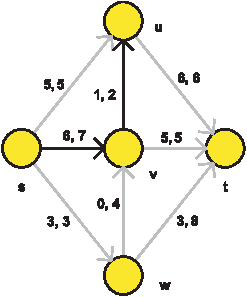
\includegraphics[width=45mm]{spolecne/08/images/toky}
    \vspace{-10px}
  \end{center}
\end{wrapfigure}

\paragraph{Řez} je množina vrcholů, ve které je zdroj ale není spotřebič Minimální řez je řez s minimální kapacitou, který odděluje zdroj a spotřebič.

\textbf{Spočítá se Ford-Fulkensonem} - vezmu TRUE vrcholy, když už nemůžeme najít zlepšující se cestu. Sečtu toky hran, které mi znemožnili zlepšení (tzn. ty které jsou nasycené, i ty zpětné!). \textbf{Kapacita řezu} je \textbf{rovna} velikosti \textbf{maximálního toku}.

V příkladě na obrázku chceme najít minimální řez. O něm víme, že jeho vrcholy získáme pomocí značkovací metody Ford-Fulkensona. Ta nejdřív označí zdroj, pak označí vrchol $v$, protože jinam nemůže (všude je nasyceno). Následně označí vrchol $u$ a z něho dál již nelze jít (všude je opět nasyceno). Tím jsou určeny vrcholy řezu ($\{s,v,u\}$).

Kapacita min. řezu je určena jako součet toků hran, které zabránili zlepšení (a nevedou uvnitř řezu). Tzn. hrana 6/6, 5/5, 0,4 a 3/3. Toky hran které \uv{odchází} sečteme, a toky zpětných hran (které přichází) odečteme $\rightarrow 6 + 5 - 0 + 3 = 14$. Kapacita řezu je rovna 14, stejně tak jako hodnota maximálního toku.

Párování je množina hran, kde žádné dvě nemají společný vrchol. Nebo také rozdělení vrcholů na dvě skupiny kde uvnitř skupiny nejsou hrany. Používá se k přiřazování lidí k taskům. Jde převést na toky nebo Maďarským algoritmem.

Tokama lze řešit velké množství problémů:

\begin{itemize}[itemsep=0px]
\item transport zásob
\item zaokrouhlování v excelu
\item multiprocesorové rozvrhování
\end{itemize}

\subsection{Multi-komoditní toky}
Tok, kde teče víc komodit. Řeší se pomocí LP nebo ILP - nutné nadefinovat Kirchhoffův zákon pro každou komoditu. 
%!TEX root=../oi-magistr-spolecne.tex
\section[KO - SPT, TSP, knapsack]{Nejkratší cesty. Úloha obchodního cestujícího. Heuristiky a aproximační algoritmy. Metoda dynamického programování. Problém batohu. Pseudo-polynomiální algoritmy.}

\subsection{Problém nejkratší cesty}

Nejkratší cesta je problém nalezení nejkratší cesty z $x$ do $y$. V obecném grafu se zápornými cykly je to NP-úplná úloha.

\paragraph{Bellmanova rovnice:} Polynomiální řešení problému nejkratších cest je založeno na Bellmanovu principu optimality, který říká, že \textbf{pokud} graf \textbf{neobsahuje cyklus záporné délky}, tak pro každé tři vrcholy $x, y, z$ platí:

$$u(x, y) = \min_{x \neq y} (u(x, z) + a(z, y))$$

Kde $u(x, y)$ značí délku cesty z vrcholu $x$ do vrcholu $y$ a $a(z, y)$ značí vzdálenost vrcholu $z$ od vrcholu $y$ (tj. délku nejkratší hrany, která tyto vrcholy spojuje).

Z Bellmanovy rovnice jednoduše řečeno vyplývá, že se každá \textbf{nejkratší cesta skládá z nejkratších cest} – tj. nejkratší cesta $[a, \cdots , x, \cdots , c]$ mezi uzly $a$ a $b$ obsahuje také nejkratší cestu mezi uzly $a$, $x$ a $x$, $c$.

Polynomiální algoritmy pro nejkratší cesty:

\paragraph{Dijkstra: $O(E\cdot \log V)$} Funguje \textbf{pokud nejsou záporné hrany}. Algoritmus má uzly v prioritní frontě podle vzdálenosti od zdroje. Na začátku zdroj 0, ostatní nekonečno. Vždy odebere uzel s nejmenší vzdáleností a provede tzv. relaxaci - podívá se na všechny sousedy ještě ve frontě a ověří, jestli se tam přes tento uzel nejde dostat rychleji. Pokud ano, sníží prioritu. Když odebereme cílový uzel, algoritmus končí. Je dobré si zaznamenávat předchůdce.

\paragraph{Bellman-Ford: $O(E\cdot V)$} Podobný Dijkstrovi, ale funguje pro hrany záporné délky. Může také \textbf{detekovat záporný cyklus}. 

Základem Bellman-Fordova algoritmu je operace relaxace. Do této operace vstupují dva uzly a hrana, která mezi nimi vede. Pokud je vzdálenost zdrojového uzlu sečtená s délkou hrany menší než aktuální vzdálenost cílového uzlu, tak se za předchůdce cílového uzlu na nejkratší cestě označí zdrojový uzel (a vzdálenost cílového uzlu se přepočítá). V případě nesplnění nerovnosti tato hrana cestu nezkracuje a neprovádí se proto žádné změny.

Délka cesty ze zdrojového do každého z cílových uzlů může být dlouhá maximálně |V|-1 hran (protože by jinak musela obsahovat cyklus). Proto pokud pustíme operaci relaxace na všechny hrany grafu |V|-1 krát, tak již musí být nalezeny všechny nejkratší cesty. Toto ověříme ještě jedním spuštěním relaxací všech hran. Pokud dojde k nějaké relaxaci, tak graf obsahuje cyklus záporné délky, pokud k relaxaci nedojde, algoritmus může vrátit výsledek.

\paragraph{Floyd-Warshall: $O(E^2 \cdot V)$} Najde nejkratší cesty od všech uzlů ke všem, detekuje záporné cykly. Nejdřív matice kdo s kým sousedí, iteruju $k=1..n$. Procházím všechny prvky a dívám se co protínám v k-tém řádku a sloupci. Sečtu ty prvky. Když je součet menší, nahradím. Při náhradách je dobré vést matici předchůdců. Když bude $<0$ na diagonále - záporný cyklus.

\paragraph{Existence hamiltonovské kružnice} Je neorientovaný graf a máme rozhodnout, zda existuje HC (kružnice která navštíví každý vrchol přesně jednou). Je to \textbf{NP-úplný problém}.

\subsection{Úloha obchodního cestujícího (TSP)}

Problém je NP-úplný a silně NP-obtížný, což znamená, že pokud platí $P \neq NP$, pak pro problém obchodního cestujícího \textbf{neexistuje} žádný polynomiální \textbf{k-aproximační} algoritmus - neexistuje polynomiální algoritmus, který by našel libovolné řešení, které je nejhůře k-násobkem optimálního řešení.

\paragraph{Důkaz NP-hard:} \hl{Redukcí z existence Hamiltonovské kružnice.}

Mějme neorientovaný graf $G$, kde rozhodujeme jestli tam je hamiltonovská kružnice. Vytvoříme instanci TSP tak, že vytvoříme uplný graf $K$. Každý vrchol z $G$ je přiřazen jednomu vrcholu v $K$. Cena hran $\{i,j\}$ v $K$ je rovna:

\begin{align*}
c(\{i,j\})=\begin{cases}
    1 & \text{pokud hrana $\{i,j\}$ je v $G$}\\
    2 & \text{pokud hrana $\{i,j\}$ není v $G$}
  \end{cases}
\end{align*}

$G$ má hamiltonovskou kružnici právě tehdy, když optimální řešení TSP se rovná $n$. $\Rightarrow$ TSP je silně NP-hard.

\subsubsection{Metrický obchodní cestující}
Variantou tohoto problému je problém metrického obchodního cestujícího, ve kterém vzdálenosti na grafu splňují trojúhelníkovou nerovnost. Toto zjednodušení odpovídá velkému množství reálných problémů (např. hledání na mapě), a zároveň umožňuje konstrukci aproximačních algoritmů.

\paragraph{2-aproximační algoritmus:} \hl{Nalezne se kostra Kruskalem a vypíše se první výskyt uzlů při procházení do hloubky.}

Algoritmus nejprve zkonstruuje minimální kostru grafu. Z definice kostry plyne, že  cena(kostra) $\leq$ cena(optimum) protože kostra obsahuje $\vert V \vert -1$ minimálních hran, zatímco kružnice jich obsahuje $\vert V \vert$.

V druhém kroku projde algoritmus kostru z libovolného uzlu do hloubky a poznamená si všechny průchody přes vrcholy - protože se jedná o průchod do hloubky, budou zde některé uzly zpracovány vícekrát.

V posledním kroku - zkrácení cest - algoritmus tento seznam projde a vynechá všechny duplicity (zanechá pouze první výskyty uzlů). Tímto dojde k vytvoření samotné kružnice.

\begin{figure}[h]
    \begin{center}
        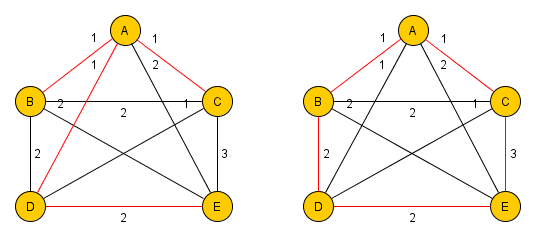
\includegraphics[width=100mm]{spolecne/09/images/tsp-2aprox}
    \end{center}
    \caption{2-aproximační alg pro TSP: např. A,B,D,E,C}
\end{figure}

\paragraph{3/2-aproximační algoritmus (Christofidesův):}
Christofidesův algoritmus řeší problém metrického obchodního cestujícího tak, že je výsledná trasa v nejhorším případě dlouhá 3/2 délky trasy optimálního řešení. Toto zlepšení je ovšem vykoupeno výrazně obtížnější implementací, a zároveň se na reálných datech ukazuje, že výsledek není v průměrném případě o mnoho lepší než při použití 2-aproximačního algoritmu uvedeného výše.

Christofidesův algoritmus nejprve zkonstruuje \textbf{minimální kostru grafu}. Poté kostru \textbf{projde} z libovolného uzlu \textbf{do hloubky} a \textbf{vybere} ty \textbf{uzly}, jež mají \textbf{lichý stupeň} a zkonstruuje na nich \textbf{úplný graf} G. Na grafu G nalezne \textbf{nejlevnější perfektní párování} $P$. Hrany z $P$ přidá do minimální kostry. Graf $K \cup P$ je nyní \textbf{eulerovský} (tzn. existuje v něm tah, který obsahuje všechny hrany grafu). Algoritmus nyní nalezne eulerovský tah – výsledná trasa odpovídá pořadí prvních návštěv uzlů při konstrukci tohoto tahu.

\subsection{Batoh (Knapsack)}
Problém batohu (Knapsack) řeší problém, které předměty dát do batohu tak, aby nebyla překročena kapacita $W$ a celková cena $C$ byla maximální.

\paragraph{2-aproximační alg $O(n^2)$} Předpokladem je, že každý z předmětů má nižší váhu než je kapacita batohu $W$ (těžší můžeme vypustit). A součet těchto vah je naopak větší než kapacita batohu (kdyby měli menší nebo roven, tak již máme optimální řešení).

\begin{enumerate}
\item Seřadíme sestupně předměty podle jejich poměru cena/váha $\frac{c_i}{w_i}$
\item Z takto seřazených předmětů vezmeme nejmenší část předmětů $h$, která přeleze přes kapacitu $W$, tzn. $h = \min\{j \in \{1,\hdots n\} : \sum\limits^{j}_{i = 1} w_i > W\}$
\item Nakonec se vezme lepší ze dvou řešení $\{1,\hdots, h-1\}$ nebo $\{h\}$
\end{enumerate}

\subsection{Dynamické programování}
Algoritmus, kde jsou udržovány mezivýsledky (něco jako cache na výsledky), které jsou dále využívány.

\paragraph{Dynamické programování na problém batohu}
Dynamické programování může vyřešit pseudo-polynomiálně. Mám tabulku číslo rozhodnutí x váha. Vždy se větvím na dva - přidám nebo nepřidám. Posunu se dolů o 1 a vpravo kolik tím přibyde váhy. Když překročím kapacitu, ořez. Do políček zapisuju celkovou cenu. Když už na políčku něco je, nahrazuji jenom menší cenu. Nejvíc vpravo dole bude optimální řešení.

\begin{figure}[h]
    \begin{center}
        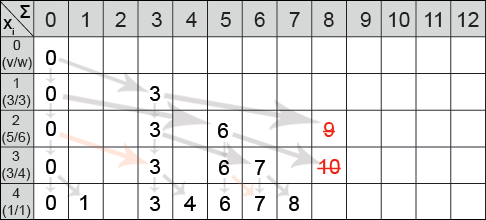
\includegraphics[width=100mm]{spolecne/09/images/knapsack}
    \end{center}
    \caption{Batoh o kapacitě 8 a předměty s váhami: $[3,6,4,1]$, hodnotami $[3, 5, 3, 1]$}
\end{figure}

\subsection{Pseudo-polynomiální algoritmy}
Pseudo-polynomiální algoritmy mají složitost $O(c \cdot n)$, kde $c$ nezáleží na velikosti instance ($n$) a může být hodně velké, až exponenciální. Např. algoritmus dynamického programování pro Knapsack.

%!TEX root=../oi-magistr-spolecne.tex
\section[KO - Scheduling]{Rozvrhování na jednom procesoru a na paralelních procesorech. Rozvrhování projektu s časovými omezeními. Programování s omezujícími podmínkami.}


\subsection{Rozvrhování}
Rozvhrování obecně je přiřazení úloh zdrojům v čase. Na vstupu je typicky množina úloh k rozvržení, každá z nich má své parametry (délka zpracování, termín dokončení apod.). Dále jsou v problému zdroje (typicky nějaké stroje nebo lidská síla), ty jsou určeny počtem (kapacitou) a každý jednotka zdroje může mít v čase přiřazen max. jednu úlohu. Cílem je rozvrhnout (přiřadit) všechny úlohy v čase při dodržení všech omezení. Přičemž rozvrh by měl být v nějakém smyslu optimální - to určuje kriteriální funkce (např. minimální délka rozvrhu).

\paragraph{Některé parametry:}
\begin{itemize}[itemsep=0px]
\item \textbf{release time} $r_j$ - čas, kdy úlohu lze nejdřív rozvrhnout
\item \textbf{process time} $p_j$ - doba zpracování
\item \textbf{due date} $d_j$ - termín, kdy by úloha měla být dokončena
\item \textbf{deadline} $\widetilde{d_j}$ - termín, kdy úloha musí být dokončena
\item \textbf{start čas} $s_j$, \textbf{čas dokončení} $c_j$
\item \textbf{čas čekání} $w_j = s_j - r_j$
\item \textbf{lateness} $L_j$ - rozdíl doby dokončení od due datu $c_j - d_j$
\item \textbf{tardiness} $D_j$ - zpoždění = doba dokončení po due datu $\max\{c_j - d_j,0\}$
\end{itemize}

\begin{figure}[h]
    \begin{center}
        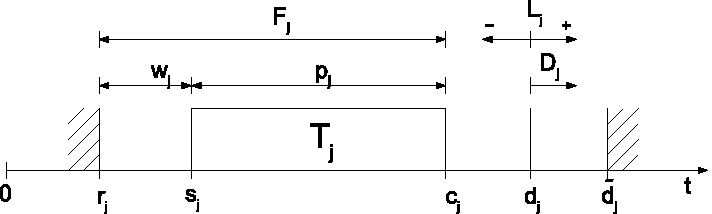
\includegraphics[width=100mm]{spolecne/10/images/scheduling-params}
    \end{center}
\end{figure}

\paragraph{Notace rozvrhovacích problémů:} $\alpha | \beta | \gamma$ (příklad: $1|r_j,d_j|C_{max}$)
\begin{itemize}
\item $\alpha$ - popisuje zdroje, jejich počet a typ (paralelní,uniformní, unrelated, job shop, atd)
\item $\beta$ - popisuje omezení jobů (precedence, preempce, due dates, deadlines, process times)
\item $\gamma$ - popisuje kritérium rozvrhu - délka rozvrhu ($C_{max}$), lateness, tardiness
\end{itemize}

\subsection{Rozvrhování na jednom procesoru}
Mnoho \uv{easy} problémů ($1|prec|C_{max}$, $1||C_{max}$, $1|r_j|C_{max}$, $1|\widetilde{d_j}|C_{max}$) - jen seřadíme úlohy např. podle $\widetilde{d_j}$. Kombinace $1|r_j,\widetilde{d_j}|C_{max}$ už není tak jednoduchá (NP-hard).

\paragraph{Bratleyův B\&B alg} Řeší \textbf{$1|r_j,\widetilde{d_j}|C_{max}$} které je \textbf{NP-hard}. Klasický branch\&bound, když překročíme deadline, můžeme odříznout i bratry. Když narazíme na řešení, zkusíme test optimality - má první úloha nejmenší release time? Jestli jo, break jinak jedeme dál.

\begin{figure}[h]
    \begin{center}
        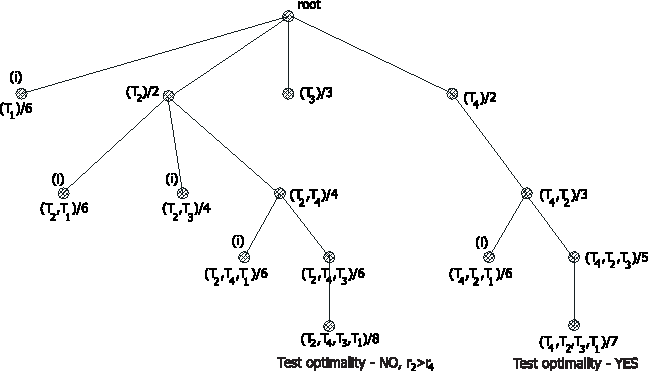
\includegraphics[width=130mm]{spolecne/10/images/bratley}
    \end{center}
    \caption{Bratleyův alg pro: $r=[4,1,1,0], p=[2,1,2,2], \widetilde{d}=[8,5,6,4]$}
\end{figure}

$1|prec|\sum wC$ se řeší branch\&bound s LP. Definujeme problém jako LP (rozhodovací proměnná $x_{ij} = 1 $ iff úloha $i$ je předchůdce $j$), což nám dá hodnotu zbylých úloh. Ořezáváme, pokud řešení + zbylé úlohy > dosud nejlepší řešení.

\subsection{Rozvrhování na paralelních procesorech}
\paragraph{McNaughton $O(n)$} Řeší $P|pmtn|C_{max}$. Spočítám si $C_{max}$ jako maximum ze součtu časů/počet procesorů a času nejdelšího úkolu:

$$C^{*}_{max} = \max \{{{1} \over {R}} \sum^{n}_{i = 1} p_{i}, \max_{i = 1, \cdots, n} p_{i} \}$$

Nyní, když je již známá délka rozvrhu, může algoritmus přistoupit k samotnému plánování. Algoritmus iteruje postupně přes všechny úkoly a vyplňuje matici od levého horního rohu po řádcích. První úkol umístí do levého horního rohu, druhý úkol těsně za něj a tak dále. V okamžiku, kdy se některý z úkolů již nevejde celý na jeden řádek (zdroj), tak jej algoritmus přeruší (nechá na k-tém zdroji vykonat pouze koncovou část úkolu), a jeho první část rovrhne na zdroj následující.

\begin{itemize}
\item $P2||C_{max}$ NP-hard - lze převést z 2-partition problému.
\item $P|pmtn,r,d|C_{max}$ jde formulovat jako úlohu maximálního toku: Udělám si intervaly pro všechny release timy a deadliny. Každý interval bude jeden vrchol. Každá úloha bude vrchol. Od zdroje k úlohám budou mít hrany hodnotu doby trvání. Od úloh do intervalových vrcholů budou mít hrany kapacitu velikosti intervalu. Od vrcholu do zdroje je kapacita velikost intervalu * počet procesorů.
\end{itemize}

\paragraph{List Scheduling (LS) $P|prec|C_{max}$} Aproximační alg. Nejdřív dám do listu úlohy bez předchůdců. Postupně přiřazuju z listu na procesory a když to někde doběhne, dám tam další a na konec listu dám následovníky té co doběhnula. Aproximační faktor $r_{LS} = 2 - \frac{1}{R}$ (R je počet zdrojů).

\textbf{Longest processing time first (LPT) $P||C_{max}$} Vylepšení pro LS v podobě vhodného řazení úloh. Funguje stejně jako LS ale řadím list podle processing timu. Aprox faktor $r_{LPT} = \frac{4}{3} - \frac{1}{3R}$. Tento problém se dá řešit ještě pomocí pseudopolynomiálního dynamického programování Rothkopf (R-rozměrné pole).

\textbf{Rothkopf} řeší dynamickým programováním pseudopolynomiálně P||Cmax. Mám tabulky časů pro každý procesor, počet rozměrů stejně jako procesorů a zapisuju tam všechny možnosti. Na konci minimalizuju rozdíl časů na jednotlivých procesorech.

\paragraph{Úrovňový algoritmus $P|pmtn,prec|C_{max}$} řeší $P|pmtn,prec|C_{max}$ v $(n^2)$. Nejdřív ohodnotím graf následností úrovněmi.

Algoritmus nejprve zkonstruuje graf závislostí, v němž jsou úkoly vyjádřené pomocí uzlů a relace následností pomocí orientovaných hran (hrana vede vždy z předka do následníka). Dále algoritmus ohodnotí všechny uzly dle následujícího schématu (S(x) značí všechny následníky uzlu x):

$$level(j) = \max_{s \in S(j)}\{level(s)\} + p_J$$

Úroveň se počítá jako délka zpracování + maximální úroveň z následníků. Proto to je vhodné počítat zprava. Samotné rozvrhování probíhá v časových kvantech. Na každý zdroj je umístěn úkol s nejvyšší úrovní. Po obsazení všech zdrojů je spuštěno zpracování úkolů na zdrojích na časové kvantum $T$, které odpovídá času do zpracování nejkratšího z úkolů. Po vykonání tohoto kvanta je zpracovaný úkol odstraněn a u částečně zpracovaných úkolů je snížena jejich úroveň o $T$ (úroveň se skládá také z délky úkolu a ta je nyní kratší). Na zdroje jsou znovu umístěny úkoly s nejvyšší úrovní (jejichž všichni předci již byli zpracováni), což ale nemusí být nutně ty, které byly částečně zpracovány v minulé iteraci. Algoritmus terminuje v okamžiku zpracování všech úkolů.

\begin{figure}[h]
    \begin{center}
        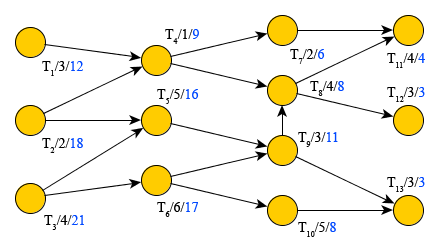
\includegraphics[width=80mm]{spolecne/10/images/level-alg}
        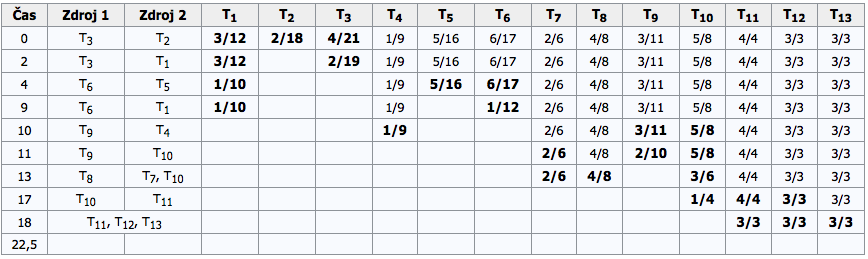
\includegraphics[width=130mm]{spolecne/10/images/level-alg-tab}
    \end{center}
    \vspace{-5px}
    \caption{Úrovňový algoritmus}
    \vspace{-5px}
\end{figure}


\subsection{Rozvrhování projektu (Project scheduling)}
Je scheduling s temporálními omezeními. $PS|temp|C_{max}$ - NP-obtížný problém. Temporální omezení jsou relace následností s váhami na hranách. Když váha = $p_j$ předchozí, můžu začít když ta předchozí skončí. Když váha > $p_j$, musím čekat. Když 0 < váha < $p_j$, musím začít během vykonávání na jiném procesoru. Řeší se pomocí ILP - binární nebo celočíselná formulace.

\subsection{Programování s omezujícími podmínkami (Constraint Programming)}
Je podobný jako ILP, ale můžeme definovat víc druhů podmínek (ILP jenom nerovnice, CSP libovolné relace). Kromě \textbf{omezení} se definují domény \textbf{pro} každou \textbf{proměnnou} - např. \textbf{sudoku} 1-9.

Postup: nejdřív udělám úvodní propagaci - aplikuji podmínky na obor hodnot. Potom jedu b\&b, postupně zkouším jednotlivé data a propaguji podmínky. Až se dostanu k nějakému řešení. Hranová konzistence znamená, že hrana s daným řešením splňuje všechna omezení.

Jeden z algoritmů pro řešení je AC-3. Při \textbf{AC3} si udržujeme \textbf{frontu hran}, které je potřeba \textbf{revidovat}. Na začátku jsou tam všechny hrany a postupně je odebíráme. Pozor, revizí nějaké hrany se může znevalidnit už validovaná hrana. Algoritmus běží, dokud nejsou všechny hrany konzistentní. Vždy reviduju přechody nejdříve v jednom směru a pak v druhém. pokud se mi změní doména (odeberu číslo), tka musím opět dát do fronty tu hranu, které se doména týká.

\begin{figure}[h]
    \begin{center}
        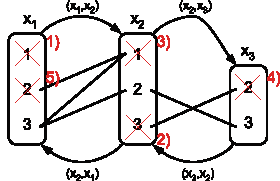
\includegraphics[width=60mm]{spolecne/10/images/ac3}
    \end{center}
    \vspace{-10px}
    \caption{AC-3: $x_1 > x_2, x_2 \neq x_3, x_2+x_3 > 4; D_1 = \{1,2,3\}, D_2 = \{1,2,3\}, D_3 = \{2,3\}$}
\end{figure}


\chapter[Zajištění kvality software]{B4M36ZKS \\[1ex]\Large{Metodika testování software. Metody vytváření testů z modelu aplikace. Automatické testování}}

Na začátek trochu slovíčkaření:

\begin{itemize}
\item \textbf{Black box testing}: Nevíme, co testujeme, nevidíme dovnitř, testy stavíme na základě pravděpodobných případů používání
\item \textbf{White box testing}: Máme k dispozici kód, děláme informované testy nebo analýzu kódu
\item \textbf{Verifikace}: Testujeme, jestli to odpovídá specifikaci
\item \textbf{Validace}: Testujeme, jestli to je to, co klient chce
\item \textbf{Regrese}: Do systému zanášíme další chyby při tom, jak se ho snažíme opravit.
\item \textbf{Test coverage}: Pokrytí testů, tedy jaká část SW je otestovaná (řádky kódu, kombinace vstupů). Vyjadřuje se v procentech.
\item \textbf{Smoke test}: Základní test funkcionality
\item \textbf{Test condition}: Něco, co testujeme, třeba funkce nebo jiná část systému. 
\end{itemize}

\paragraph{V-model} V-model je model vývoje SW od návrhu po realizaci, má dvě části, tvorbu a testování. Tvorba je business model, požadavky, funkční návrh, technický návrh, implementace. Testování jsou vývojářské testy, integrační testy, systémové testy, uživatelské akceptační testy (UAT), produkční provoz. Problém je, že čím později odhalíme chybu, tím dražší je to opravit - a pokud je ve V modelu chyba v požadavcích, odhalí to až poslední testy UAT.

\paragraph{W-model} W-model je podobný V-modelu, ale opravuje chybu s pozdním odhalením chyby. Tentokrát je nějaká forma revize nebo testu přítomná v každém kroku, tedy po požadavcích, návrhu atd.

\paragraph{Quality gates} Quality Gates jsou kontroly mezi jednotlivými kroky ve fázi tvorby V/W modelu. Buď jsou striktní, tj dokud to někdo neschválí, tak se nemůže pokračovat, nebo jsou kooperativní, kdy ten, kdo práci dokončil odpovídá na otázky tomu, kdo projekt přebírá, a všichni se ujišťují, že je vše ok.

\paragraph{Statické testování} Testujeme komponentu nebo systému na úrovni specifikace nebo implementace bez spouštění systému. Probíhá v částí Tvorby ve V-modelu. Pro specifikaci se dělají různé úrovně revizí, pro implementaci se dělá Code Review a jiné statické analýzy kódu. Revize mají čtyři úrovně:

\begin{enumerate}
\item Informal review: Neformální kontrola
\item Walktrough: Autor ukazuje dílo ostatním a komentuje to
\item Technical review: Formální, někdo to moderuje (ne autor)
\item Inspection: Formální, někdo to moderuje, je předem daný proces, pořizuje se zápis, používají se metriky atd.
\end{enumerate}

\paragraph{Jak hodnotit specifikaci} Nechceme tam mít vágní formulace: \textit{by mělo}, chybějící části: \textit{tohle, tamto, atd}, nedodělky: \textit{TODO}, nakopírované kusy, chybějící odkazy na dokumentaci. Specifikaci můžeme kontrolovat tak, že ji projdeme a na základě toho sestavíme popis aplikace (ten by měl odpovídat realitě). Dělá se to v krocích, každý krok má dvě části, a totiž návrh a kontrola. V návrhu sepíšeme vše, co jsme našli, a v kontrole ověřujeme, že vše se použije, a že to dává smysl.
\begin{enumerate}
\item Zjistit, kdo jsou uživatelé
\item Zjistit, jaké funkce systém poskytuje (a komu)
\item Namapovat uživatele na funkce
\end{enumerate}



\section{Automatizace testů}

Automatizace se vyplatí, když máme opakující se testy, různé platformy, nebo chceme testovat hodně parametrů. Jde to dělat různě: klikací automat, sekvence HTTP packetů, javascript inject do stránky, pluginy pro prohlížeč, OCRka.

Taky se dají dělat jednotkové testy (česky unit testy), kde se v kódu volají funkce a zjišťuje se, jestli vrátily to, co měly, případně jestli vyhodily správnou výjimku. Unit testy by se měly vytvářet (a spouštět) průběžně během vývoje.


\section{Výběr dat}

\paragraph{Třídy ekvivalence} Máme aplikaci, která dává slevu na základě ceny nákupu: 0-499kč žádná sleva, 500-999kč 5\% sleva, 1000kč a víc 5\% sleva a doprava zdarma. Pak nemusíme testovat všechny hodnoty, ale stačí vybrat z každého rozsahu jednu hodnotu, a navíc otestovat hraniční hodnoty. Tyhle intervaly jsou naše třídy ekvivalence, protože pro hodnoty z jednoho intervalu se bude aplikace chovat stejně. Druhým typem tříd ekvivalence (kromě intervalů) jsou diskrétní hodnoty (metoda platby, typ prohlížeče atd). Třídy ekvivalence mohou být validní (to, co aplikace očekává), nebo nevalidní (místo částky je tam string, nebo je částka záporná).

\subsection{Výběr kombinace dat} Použitím tříd ekvivalence jsme se dostali na rozumný počet dat, ale když budeme testovat nějakou funkci, musíme stejně vybrat, kolik kombinací vstupu uděláme. Dá se to nakreslit jako strom (klasifikační strom), kde v kořeni je název funkce, jako děti jsou názvy vstupních parametrů, a listy jsou možné hodnoty (tedy třídy ekvivalence). Na výběr kombinace vstupů je přibližně tisíc možných postupů, ve slidech jsou všechny, ale jen některé se vysvětlují:
\begin{description}
\item[MCC - Multiple Condition Coverage] testujeme všechny možné kombinace
\item[MC/DC - Modified Condition/Decision Coverage] testujeme všechny kombinace, které mají mít odlišný výsledek	
\item[Pairwise testing] tesujeme všechny možné dvojice dat
\item[C/DC - Condition/Decision Coverage]
\item[CC - Condition Coverage]
\item[DC - Decision Coverage]
\item[Ruční výběr] ještě menšího množství kombinací
\end{description}

Čím je postup níž v seznamu, tím má horší pokrytí. Kritické aplikace používají MCC nebo MC/DC. Existuje software, který generuje testovací sady za nás.

Příklad: Máme funkci, která má rozhodnout, jestli může pilot létat zaoceánské lety, odmínka je následující: \textit{Pokud pilot (má nalétáno víc než 200 hodin nebo absolvoval víc než 10 linkových letů) a zároveň prošel výcvikem pro let nad mořem, pak může létat na zaoceánských letech}. To jde pro účely testování zkrátit jako $R = ( A \vee B ) \wedge C$.

\paragraph{MCC} Máme tři vstupy, všechny jsou binární (má/nemá nalétáno, prošel/neprošel výcvikem). Počet MCC kombinací zjistíme tak, že vynásobíme počet variant v každé proměnné, tedy v tomto případě budeme mít $2\cdot 2 \cdot 2 = 8$ testů: 000, 001, 010, 011, 100, 101, 110, 111.

\paragraph{MC/DC} Uděláme pravdivostní tabulku a z nějakého důvodu na diagonálu pro každou proměnnou dáme nějakou hodnotu (modrá čísla). Zbylé proměnné doplníme tak, aby výsledek odpovídal hodnotě ve sloupci (černá čísla nahoře). To se dělá tak, že tam dáme \textit{neutrální hodnoty} - pro AND je neutrální hodnota 1, pro OR je to 0. V~poslední řádce to jde udělat více způsoby, tak vybereme ty, které už se tam někdy vyskytují, tedy 011 a třeba 000, to druhé je jedno). Testy, které se opakují (třeba 001) děláme jen jednou. Dostali jsme tedy testy: 101, 011, 001, 000.

\begin{figure}[ht!]
\centering
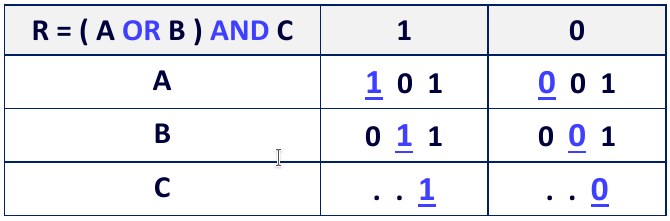
\includegraphics[width=0.5\textwidth]{ZKS/img/mcdc.png}
\end{figure}

\paragraph{Pairwise testing} Chceme vybrat každou dvojici, takže pro AB: 01, 10, 00, 11, pro BC: 01, 10, 00, 11, pro AC: 01, 10, 00, 11. To splňuje třeba sada testů: 000, 011, 110, 101. 


\section{Testy průchodu}

\paragraph{Free testing} Nevíme, jak aplikace funguje, nějak tím klikáme a zkoušíme

\paragraph{Exploratory testing} Jako free testing, ale zaznamenáváme, co jsme zkoušeli

\subsection{Pokrytí cest}

Když víme, jak aplikace funguje, tak vycházíme z vývojového diagramu. Ten si nakreslíme a popíšeme body a hrany. Pak zvolíme hloubku testu (pokrytí cest):

\begin{itemize}
\item Hloubka 1: Projdeme každou hranu aspoň jednou
\item Hloubka 2: Projdeme každou dvojici po sobě následujících hran aspoň jednou (tedy v každém bodě vyzkoušíme všechny kombinace vstupu a odchodu).
\item Hloubka 3: Projdeme každou trojici po sobě následujících hran aspoň jednou.
\end{itemize}

Pak sestavíme testy tak, abychom jich měli co nejméně, a přesto jsme pokryli všechny průchody s požadovanou hloubkou. Další možnost je \textit{Elementary comparison test}, kdy zkoušíme průchody a kombinace dat zároveň. V některých postupech (PA a ST - smoketest) se navíc pracuje s prioritami, tedy pokud si můžeme vybrat, kterou hranu projdeme víckrát, vybereme tu s vyšší prioritou.

\subsection{Konzistence dat}

Testování dle pokrytí nemusí být dostatečné pro chyby, které se týkají dat. Jedna část kódu může data poškodit, a jiná je pak nebude moci použít - přitom takový průchod vůbec nemusel být testován, i když budeme mít otestované pokrytí cest. Manipulace s daty má 4 kroky: create, read, update, delete, a říká se tomu CRUD.

Práci aplikace s daty v aplikaci se sepíše do CRUD matice, což je tabulka, kde je pro každý druh dat (objekt?) a každou funkci napsané, jaká operace se s danými daty v dané funkci dělá. Obvykle by každý objekt měl být někde vytvořen, přečten, a následně smazán, ale pokud to tak není, nevadí to, v některých případech by to nedávalo smysl.

Pro každý objekt sestavíme několik scénářů, jak se s objektem v aplikaci pracuje: typicky vytvoření, pak kombinace čtení a úprav, a pak smazání. Sestavíme posloupnost funkcí, kde se tyto akce s objektem dělají. Pak testujeme průchody aplikací tak, abychom volali ty správné funkce.
\chapter[Databáze 2]{B4M36DS2 \\[1ex]\Large{Pojem Big Data, základní principy distribuovaného zpracování dat, typy a vlastnosti NoSQL databází}}

\chapter[Softwarové Architektury]{B4M36SWA \\[1ex]\Large{Softwarové architektury, jejich parametry a kvalitativní metriky. Architektonické vzory, styly a standardy}}

\chapter[Paralelní algoritmy]{B4M35PAG \\[1ex]\Large{Vlastnosti paralelních a distribuovaných algoritmů. Komunikační operace pro paralelní algoritmy. Paralelní algoritmy pro lineární algebru. \textbf{}}}





\chapter[Bezpečnost systémů]{B4M36BSY \\[1ex]\Large{Bezpečnostní analýza operačních systémů, bezpečný vývoj software a bezpečnost webových aplikací. Analýza útoků a škodlivého kódu. Bezpečnost mobilních zařízení.}}

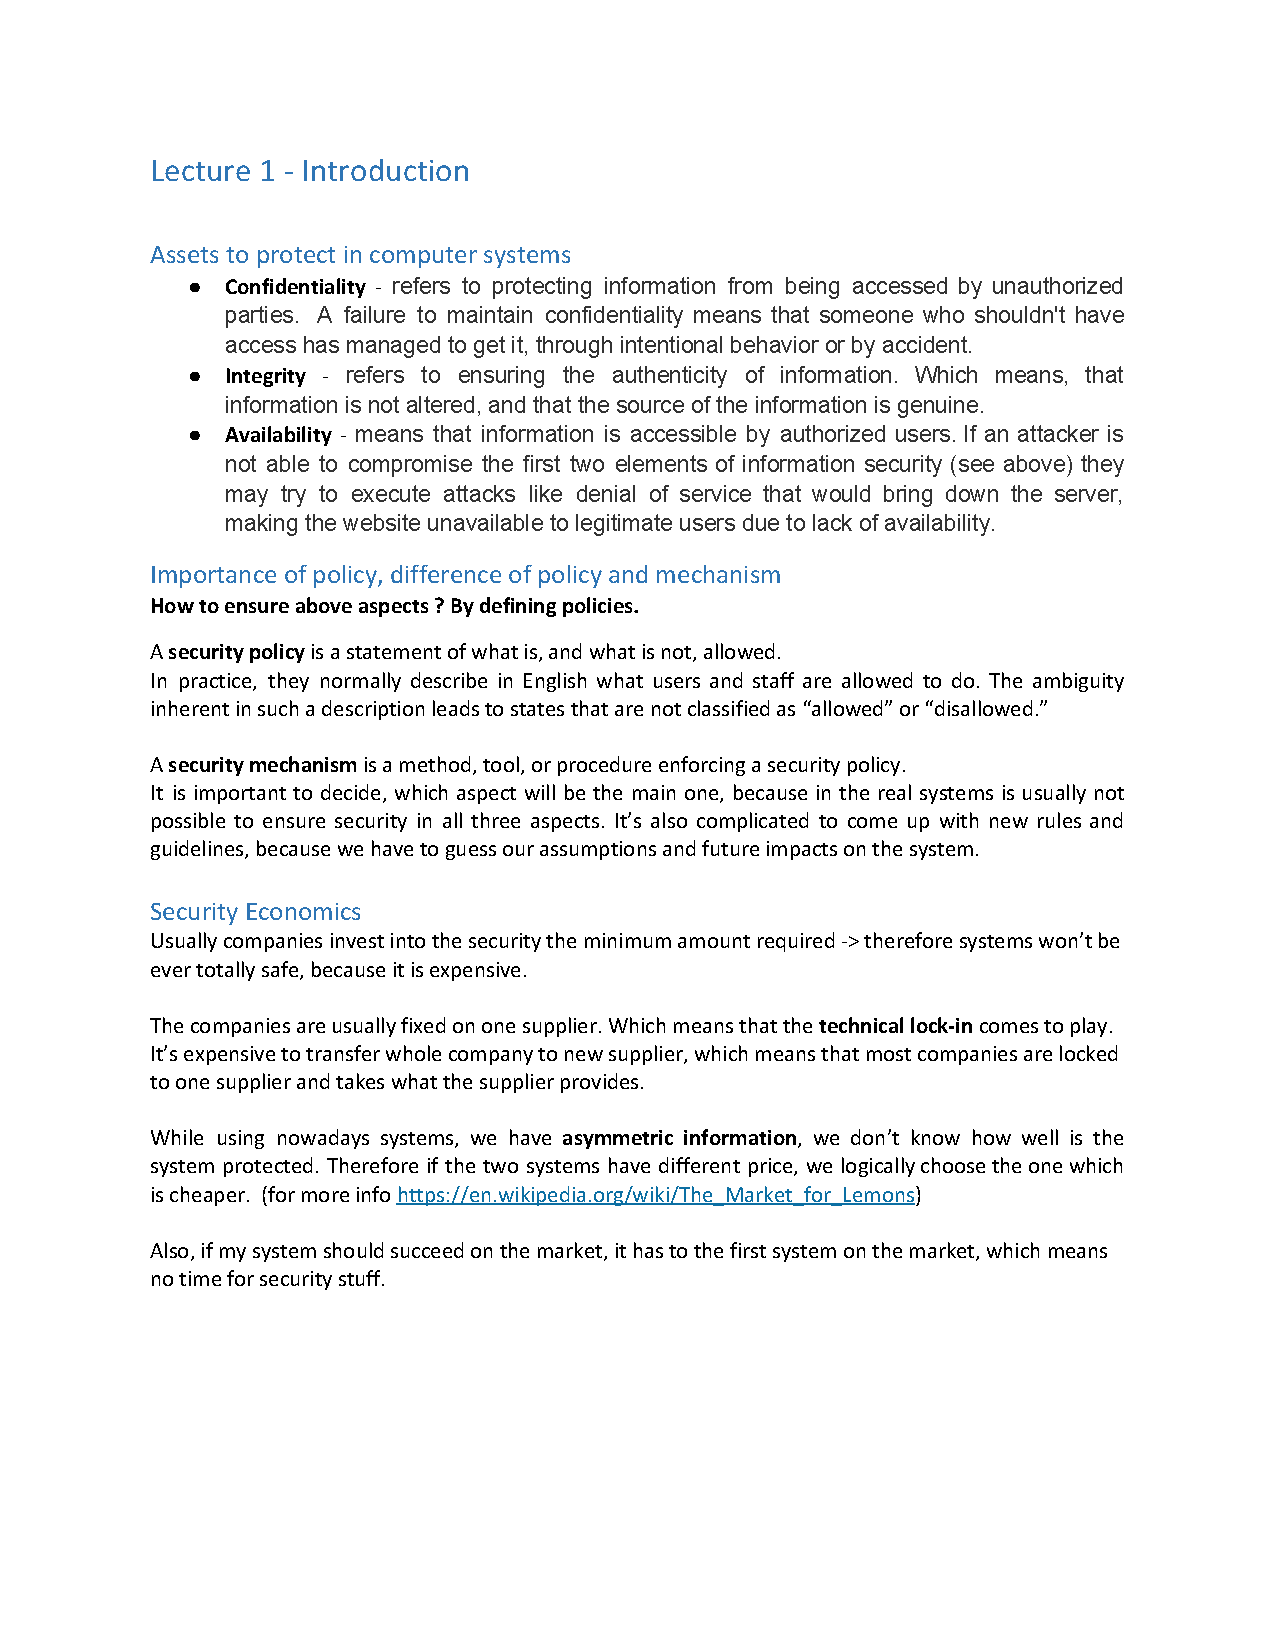
\includepdf[pages=-]{oborove/BSY/vytah.pdf}

\chapter[Efektivní Software]{B4M36ESW \\[1ex]\Large{Efektivní algoritmy a způsoby optimalizace. Datové struktury, synchronizace a vícevláknové programy.}}

\includepdf[pages=3-37]{oborove/ESW/esw_guide.pdf}

\bibliographystyle{spolecne/_lib/csplainnat}
{
    \footnotesize
    \def\CS{$\cal C\kern-0.1667em\lower.5ex\hbox{$\cal S$}\kern-0.075em $}
    \bibliography{reference}
}
\end{document}